\documentclass{article}
\usepackage{url,color,xspace,verbatim,subfig,ctable,multirow,listings}
\usepackage[utf8]{inputenc}
\usepackage[T1]{fontenc}
\usepackage{txfonts}
\usepackage{rotating}
\usepackage{paralist}
\usepackage{subfig}
\usepackage{graphics}
\usepackage{enumitem}
\usepackage{times}
\usepackage{amssymb}
\usepackage[colorlinks=true]{hyperref}
\usepackage[ruled,vlined]{algorithm2e}
\usepackage[toc,page]{appendix}
% ==================================================

\graphicspath{{figs/}}
\urlstyle{sf}

% tikz stuff
\usepackage{tikz}
\usepackage{pgfplots}
% configuration
\usetikzlibrary{shapes,positioning,calc,snakes,arrows,shapes,fit,backgrounds}
\pgfplotsset{width=.9\linewidth}

\lstset{
  language=C,
  basicstyle=\ttfamily \small,
  flexiblecolumns=false,
  basewidth={0.5em,0.45em},
  boxpos=t,
}

\newcommand{\etal}{{\it et al.}\xspace}
\newcommand{\naive}{na\"{\i}ve\xspace}
\newcommand{\Naive}{Na\"{\i}ve\xspace}
\newcommand{\textc}[1]{{\color{gray} {\footnotesize #1}}}

\definecolor{skRed}{RGB}{155,25,25}
\newcommand{\stefan}[1]{
  {\color{skRed}[{\color{red}{SK}} #1]}}

\setcounter{section}{0} % Start sections with 1, not 0
\begin{document}

\title{Adaptive broadcast tree for multicores}

% email address
\newcommand{\eaddr}{stefan.kaestle@inf.ethz.ch}
\newcommand{\email}{\href{mailto:\eaddr}{\eaddr}}

\author{Stefan Kaestle\\
  \email \\
  Systems Group, ETH Zurich}

\maketitle

% keywords: modeling, simulation, overlay networks, scheduling

%%%%%%%%%%%%%%%%%%%%%%%%%%%%%%%%%%%%%%%%%%%%%%%%%%
%%%%%%%%%%%%%%%%%%%%%%%%%%%%%%%%%%%%%%%%%%%%%%%%%%
\section{Introduction}

Distributed algorithms are increasingly used to overcome scalability
challenges on multicore machines. Examples are
databases~\cite{Salomie2011, Wiesmann2000} and operating
systems~\cite{fos:osr09, tornado:osdi99, barrelfish:sosp09}.

% What do you want to enable?
We want to investigate how to achieve better performance of atomic
broadcast across a wide range of multicore machines without manually
tuning the implementation to concrete machines.

% What problem are you solving, and why is it hard?
The problem is complexity and diversity of modern multicore
machines. Multicores come in many flavors depending on vendor and
generation of the machine. All of these machines have fundamentally
different characteristics such as number of nodes, NUMA
characteristics, interconnect topologies, propagation time on
interconnect and use of shared caches. These characteristics are hard~\cite{Cavage2013}
to understand, but important to consider for application performance. 

% New ideas
Instead of manually tuning algorithms to characteristics of individual
machines, we automatically configure distributed algorithm
implementations based on a machine model. We represent this model as an
annotated graph. One question we are looking at is which information
should actually be part of this machine model.

% How will you go about it?
We base the configuration of algorithms on \emph{overlay networks}, which we
automatically configure. We execute our configuration stage on a model
representing the concrete machine the algorithm is intended to run
on. %
Our idea is to then explore different approaches for finding overlay
networks based on the network model graph. Approaches we are currently
investigating are: minimum spanning tree algorithms, binary trees,
clustering techniques as well as treating the problem
hierarchically. Assuming the overlay network, we then need to decide
on every node which message to send first. This is a \emph{scheduling}
problem.

% How do we show it works
We auto-configure a wide range of different multicore machines and
compare the performance of our implementation with hand-tuned
implementations on all of these machines.
% Hypothesis
Our hypothesis is that automatic tuning of distributed algorithms 
to machine characteristics is worth
doing. Obviously, we cannot achieve performance of hand-tuned
implementations, but we hope to get close enough to argue that loosing
a bit of performance to avoid tedious manual reconfiguration is worth
if for many applications (while others, where performance
\emph{really} matters, might still want to manually configure their
stuff).

% three-step approach
We break the problem down into three steps:
\begin{inparaenum}[\itshape 1\upshape)]
\item We first represent multicore machines by a model. We describe
  this model in Section~\ref{sec:model},
\item We then find an overlay for a concrete network model. This
  overlay network describes a topology (such as a tree or a ring) for
  communication within the machine. Algorithms to select overlay
  networks are described in Section~\ref{sec:overlay}, and
\item Given the overlay, we need to decide for every node in which
  order to send messages. We investigate this scheduling problem in
  Section~\ref{sec:scheduling}.
\end{inparaenum}

\begin{figure}[htb]
  \centering
  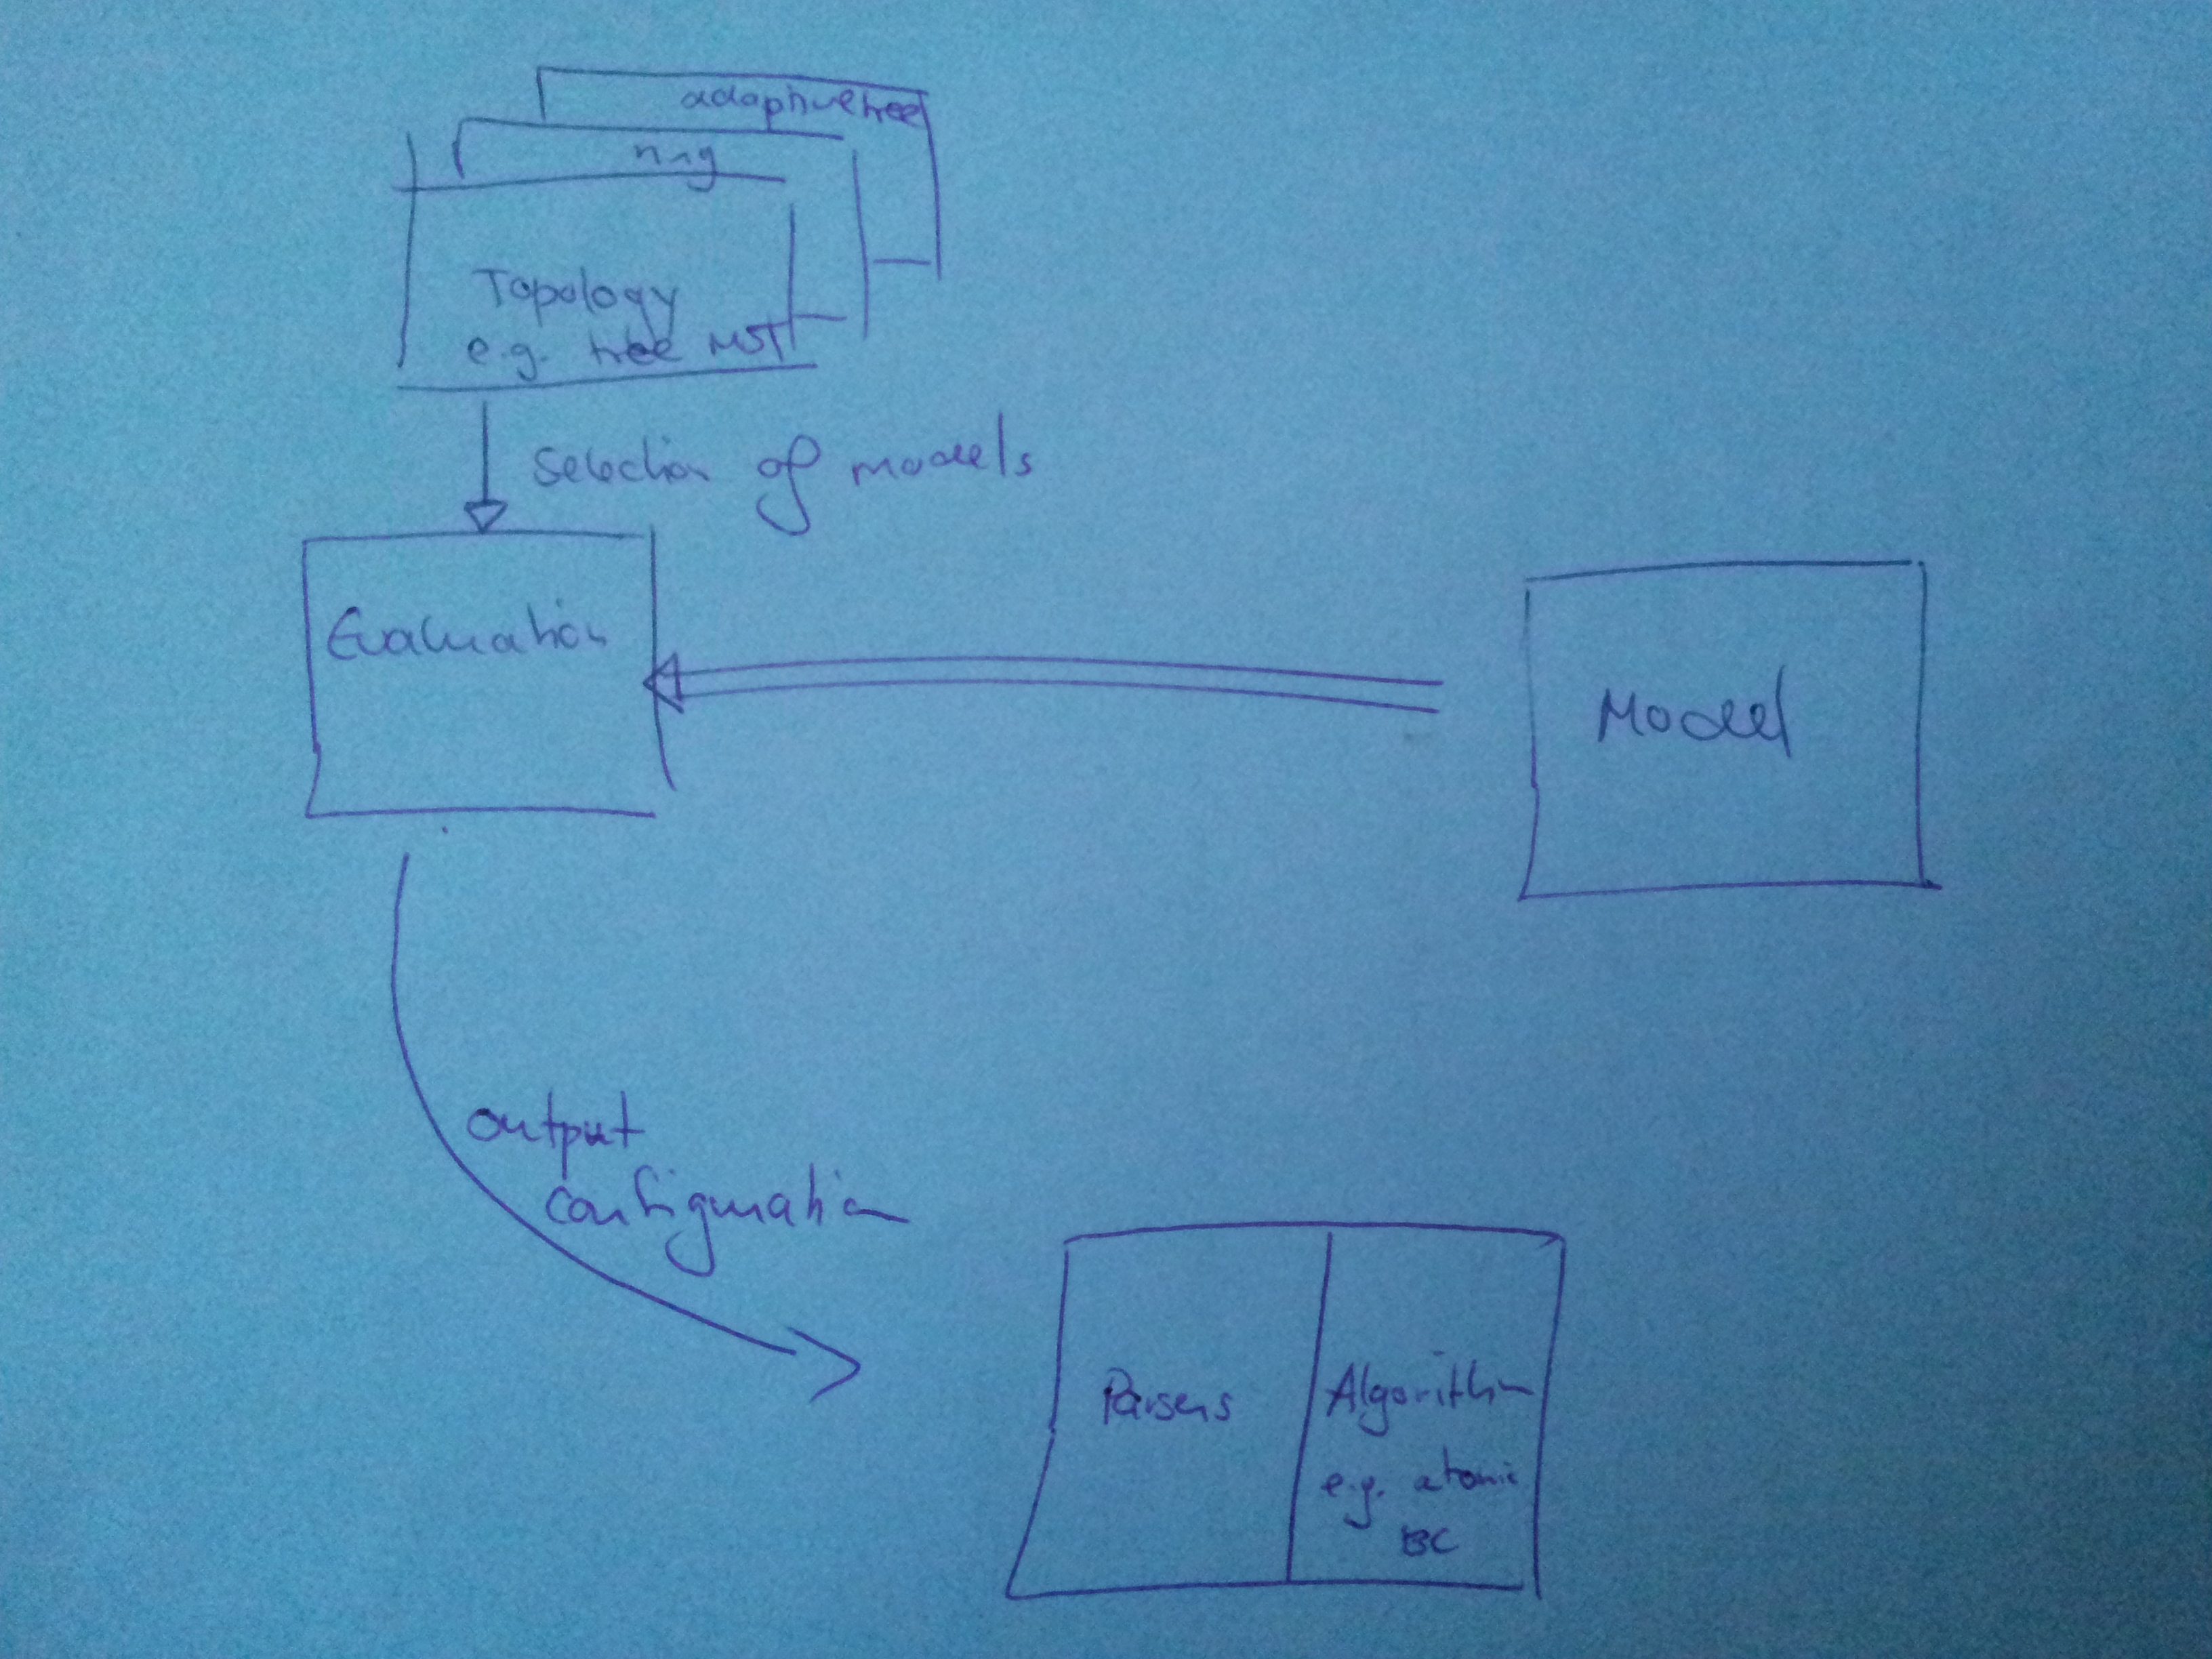
\includegraphics[width=\linewidth]{Overview_Model_Evaluation_Parser}
  \caption{Overview of configuration of atomic broadcast using a Model 
    \stefan{Draw figure properly}}
  \label{fig:overview}
\end{figure}

%%%%%%%%%%%%%%%%%%%%%%%%%%%%%%%%%%%%%%%%%%%%%%%%%%
%%%%%%%%%%%%%%%%%%%%%%%%%%%%%%%%%%%%%%%%%%%%%%%%%%
\section{Distributed algorithms}
\label{sec:distalgo}

In order to evaluate our ideas, we pick two concrete distributed
algorithms and implement them for a multicore machine:

\paragraph{Atomic broadcast} An Atomic broadcasts is a broadcast
messaging protocol that is reliable in the sense that if a message is
received by one of the participating nodes, it is also received by all
other nodes. Furthermore, the order of messages as seen by all
participants is the same. Atomic broadcasts are frequently used to
implement higher-level distributed algorithms on top of it: examples
are replication such as state machine replication. As a first step, we
evaluate the performance of sending one message as a broadcast to all
nodes. Broadcasts are one of the most important communication
operations for parallel applications~\cite{Bruck1992}. \stefan{Database
  joins}.

\paragraph{Barriers} \stefan{Explain}

%%%%%%%%%%%%%%%%%%%%%%%%%%%%%%%%%%%%%%%%%%%%%%%%%%
%%%%%%%%%%%%%%%%%%%%%%%%%%%%%%%%%%%%%%%%%%%%%%%%%%
\section{The multicore network model}
\label{sec:model}

% selecting hard
Characteristics of the network influence the performance of
distributed algorithms. 
% model
We express these network characteristics in a multicore network
model. This model at this stage is by no means complete. We are going to
extend it over time to address more complexities of current and future
multicores.
% static
Our network model is \emph{static}, which in particular implies that
we do not consider run-time effect such as congestion for the moment.

% graph
We represent the multicore network as a \emph{directed graph}. The nodes in
this graph correspond to cores, and edges to communication channels
between nodes. The machines we consider for now only have
bi-directional communication links. Other machines (like the SCC) have
uni-directional links, which is why we model the graph as directed
graph.
% shared memory -> fully meshed
This graph is \emph{fully meshed} for shared memory machines. Every core can
communicate with every other node via the cache coherence protocol.

% machines hierarchical
Multicore machines are hierarchical. Processor cores are grouped in
NUMA nodes with shared caches. These NUMA nodes are then connected to
each other by increasingly complex interconnect networks. 
% NUMA affinity -> model
We encode NUMA node affinity in our model. This allows to break down
programming of a multicore machine into two distinct instances. We
solve one instance of the problem between NUMA nodes, and then, in a
second step, within each NUMA node. These two steps can be executed
independently and different algorithms can be used in both case.

% why it makes sense?
If cores on the same NUMA node share a cache, it makes sense to
leverage this hardware feature to implement shared-memory algorithms
on top of it. %
Communication across NUMA nodes is realized sending messages across
the packet-based interconnect network. Using message-passing based
implementations is the natural choice. %
Shared memory algorithms and message-passing based algorithms can be
composed together to program hierarchical machines similarly to what
was previously shown for composing of shared-memory
algorithms~\cite{Alistarh2012}.

%%%%%%%%%%%%%%%%%%%%%%%%%%%%%%%%%%%%%%%%%%%%%%%%%%
\subsection{Node characteristics} 
\label{sec:model_nodes}

\stefan{Not sure yet if we really need this, but it should be helpful
  for treating the machine hierarchically}

Every node (i.e.\ core) in the system has characteristics associated
with it.

\begin{description}
\item[NUMA affinity] A list of cores on the same NUMA node.
\item[Synchrony] Synchronous systems are characterized by two
  attributes: First, cores execute their programs in lock-steps and
  second that message delivery time is bound.
  % 
  The existence of lock-steps implies the existence of a global time.
  This is often true on multicore machines since cores are driven by
  the same quartz or, if not, they are synchronized such that the
  jitter is less than a cycle, which leads to cores seeing the same
  time. %
  Bounded delivery time is harder to reason about. CPUs on multicores
  are typically time-multiplexed. On such systems, several programs
  execute on the same processing unit one at a time. A scheduler
  decides the order in which to run these applications. In very
  contented systems, timely receipt of messages cannot be guaranteed
  globally for all applications since many of them compete for a CPU
  core. Even if we could guarantee timely delivery of messages by use
  of a deterministic scheduler, worst-case propagation times would
  still be orders of magnitude higher than best-case propagation
  (which is essentially zero). \stefan{gang-scheduling?}
\item[Failure] Can nodes fail? If so, how? (Byzantine, crash). We do
  not consider failures at the moment, but believe that we will
  inevitably have to do so for future multicores, where it is unlikely
  that hardware can hide failures from software.
\end{description}

%-------------------------------------------------
\subsection{NUMA characteristics}
\label{sec:model_numa_nodes}

\stefan{Maybe characteristics of NUMA nodes do not have to be encoded
  separately, but as part of the node characteristics?}

Some characteristics of multicore communication stem from the NUMA
hierarchy. Thus, such characteristics can be encoded separately in the
model.

\begin{description}
\item[hop count] Number of hops to every other NUMA node. The cost of
  sending a message in a multicore machines does not so much depend on
  the distance on the interconnect networks as on the number of hops
  on such a path. Propagation on the wire is essentially for free due
  to short distances between cores. %
  On a multi-hop path, however, packages traversing the interconnect
  need to be buffered. This is expensive. Depending on the machine,
  some routing is executed on every intermediate route, which
  increases the latency further.
\item[hop count histogram] For every NUMA node, we want to know how
  many other NUMA nodes can be reached with $n$ hops. This tells us
  something about how well such nodes are connected to other NUMA
  nodes. The intuition is that it makes sense to send a message to a
  well connected NUMA node early in time, to ``spread'' out a message
  as quickly as possible.
\end{description}

%%%%%%%%%%%%%%%%%%%%%%%%%%%%%%%%%%%%%%%%%%%%%%%%%%
\subsection{Link characteristics} 
\label{sec:model_links}

The network model is defined by communication channels, which in turn
are defined by a set of attributes (here sorted by priority):

\begin{description}
\item[cost breakdown] (quantitative) of message send cost:
  dominating propagation time vs.\ dominating send and receive time on
  multicores (per-node). Our model is currently limited to only the
  breakdown of the cost for sending messages. Maybe we do not strictly
  need to know about propagation time, as it is negligible independent
  of were messages are sent. Relevant seems to be the number of hops
  rather than the latency expressed in a concrete time.
\item[bounded delivery]
\item[reliability] (loss, link failure, in-order delivery, phantoms,
  corruption, duplicated messages): 
  multicore interconnect networks often are
\end{description}

% Assumptions
We assume that the cost of sending a message to the same node is 0,
which is not true, since even using a highly optimized implementation
for local communication (like LMP) has a non-negligible cost.

% Limitations
What we do not consider yet is link congestion. 

%%%%%%%%%%%%%%%%%%%%%%%%%%%%%%%%%%%%%%%%%%%%%%%%%%
\subsection{Acquiring the model}

% Model given
We assume that the model is given. We just define one ourselves for
now or build one manually for a particular machine. In a real-world
scenario, this does not work. The model needs to be created
automatically for a particular machine (due to the diversity of
machines, and also the pace at which hardware changes)

We now make up a machine model for evaluation. This model is based on
a 8x4x1 AMD Shanghai machine. The topology of such a machine is shown
in Figure~\ref{fig:gruyere}.

Each of the eight NUMA nodes consists of four cores. We approximate the
cost of sending messages within nodes as $1$ and across nodes as
$10*num(hops)$.

Send and receive time are $10$ each, i.e.\ in the order of propagation
over a cross-NUMA link.

\begin{figure}[htb]
  \centering
  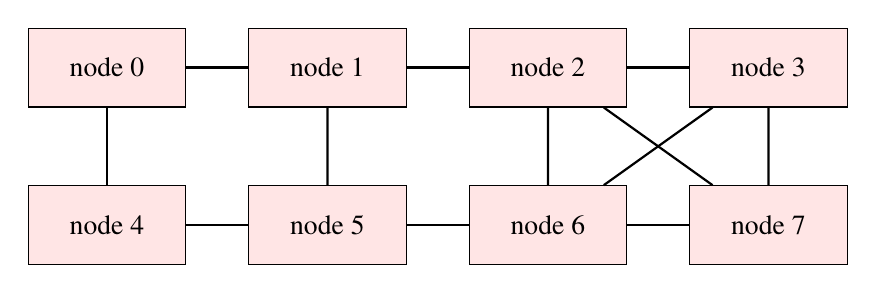
\begin{tikzpicture}[
    xscale=.7,
    yscale=.5,
    every node/.style={draw,fill=red!10,minimum width=2cm,minimum height=1cm}
    ]
    \node (c1) at ( 0, 4) {node 0};
    \node (c2) at ( 4, 4) {node 1};
    \node (c3) at ( 8, 4) {node 2};
    \node (c4) at (12, 4) {node 3};

    \node (c5) at ( 0, 0) {node 4};
    \node (c6) at ( 4, 0) {node 5};
    \node (c7) at ( 8, 0) {node 6};
    \node (c8) at (12, 0) {node 7};

    % top horizontal
    \draw[thick] (c1) -- (c2);
    \draw[thick] (c2) -- (c3);
    \draw[thick] (c3) -- (c4);
    % bottom horizontal
    \draw[thick] (c5) -- (c6);
    \draw[thick] (c6) -- (c7);
    \draw[thick] (c7) -- (c8);
    % vertical
    \draw[thick] (c1) -- (c5);
    \draw[thick] (c2) -- (c6);
    \draw[thick] (c3) -- (c7);
    \draw[thick] (c4) -- (c8);
    % cross
    \draw[thick] (c3) -- (c8);
    \draw[thick] (c4) -- (c7);
  \end{tikzpicture}
  \caption{Interconnect topology of 8x4x1 AMD Shanghai machine}
  \label{fig:gruyere}
\end{figure}

%%%%%%%%%%%%%%%%%%%%%%%%%%%%%%%%%%%%%%%%%%%%%%%%%%
%%%%%%%%%%%%%%%%%%%%%%%%%%%%%%%%%%%%%%%%%%%%%%%%%%
\section{Overlay selection}
\label{sec:overlay}

For a specific model, we now need to find ``the right'' implementation
of algorithms to program it. We build our atomic broadcast based on a
subset of links offered by the model such that all nodes of a given
multicore machine can be reached. Atomic broadcast guarantees that 1)
if one node receives a message, all other nodes receive it as well,
and 2) that all nodes see the message in the same order.

First, we discuss what kind of topologies we use to communicate
between nodes. We evaluate tree based implementations: binary trees,
minimum spanning trees, hierarchical tress and clustering
techniques. Other potentially interesting topologies are rings.

%%%%%%%%%%%%%%%%%%%%%%%%%%%%%%%%%%%%%%%%%%%%%%%%%%
\subsection{Tree Topology}

We now look at tree-based atomic broadcast implementations. The first
challenge is to find efficient spanning trees for arbitrary
machines. We now discuss different strategies to select trees based on
the model representing the machine.

Several optimizations are possible. First, nodes further up the tree
should have a higher degree i.e.\ send more messages so that they do
not idle~\cite{Bar-Noy1994}. An example of such a tree is a Fibonacci
tree, which is known to be optimal for the case that send and receive
time are equal~\cite{Bar-Noy1994}. 

In contrast, we assume that the model is given, which allows us to
simulate sending messages along the broadcast tree. Whenever a node is
idle in the model, it will send a message to one of the cores, that
did not receive any messages yet. For the special case that send
equals receive time, this should also yield a Fibonacci tree.

%-------------------------------------------------
\subsubsection{Binary Tree}

A very \naive strategy to build a tree from machine models is the use
of a binary tree with root in core 0. Every node $n$ has two children
$2(n+1)-1$ and $2(n+1)$.

The benefit of such a tree is that the time complexity is guaranteed
to be $O(\log{n})$. The downside is that it is not considering the
machine topology. Unnecessary communication across NUMA nodes might be
introduced. 

We show an example for such a tree for a 8x4x1 AMD Barcelona machine
(gruyere) in Figure~\ref{fig:qrm_tree_gruyere}.

\begin{figure}
  % Start of code
% \begin{tikzpicture}[anchor=mid,>=latex',line join=bevel,]
\begin{tikzpicture}[>=latex',line join=bevel,scale=.35]
  \pgfsetlinewidth{1bp}
%%
\pgfsetcolor{black}
  % Edge: 15 -> 31
  \draw [->] (27bp,74.327bp) .. controls (27bp,66.264bp) and (27bp,56.648bp)  .. (27bp,37.667bp);
  % Edge: 9 -> 19
  \draw [->] (459bp,148.33bp) .. controls (459bp,140.26bp) and (459bp,130.65bp)  .. (459bp,111.67bp);
  % Edge: 14 -> 30
  \draw [->] (1050.3bp,151.31bp) .. controls (1060.4bp,140.94bp) and (1073.7bp,127.18bp)  .. (1092bp,108.42bp);
  % Edge: 14 -> 29
  \draw [->] (1035bp,148.33bp) .. controls (1035bp,140.26bp) and (1035bp,130.65bp)  .. (1035bp,111.67bp);
  % Edge: 11 -> 23
  \draw [->] (659.73bp,151.31bp) .. controls (649.64bp,140.94bp) and (636.25bp,127.18bp)  .. (618bp,108.42bp);
  % Edge: 7 -> 15
  \draw [->] (83.731bp,151.31bp) .. controls (73.64bp,140.94bp) and (60.253bp,127.18bp)  .. (42bp,108.42bp);
  % Edge: 0 -> 2
  \draw [->] (588.87bp,377.76bp) .. controls (613.22bp,365.25bp) and (652.76bp,344.93bp)  .. (689.4bp,326.1bp);
  % Edge: 10 -> 22
  \draw [->] (387bp,148.33bp) .. controls (387bp,140.26bp) and (387bp,130.65bp)  .. (387bp,111.67bp);
  % Edge: 13 -> 28
  \draw [->] (935.71bp,149.09bp) .. controls (939.96bp,140.36bp) and (945.15bp,129.68bp)  .. (954.37bp,110.75bp);
  % Edge: 1 -> 3
  \draw [->] (398.64bp,306.66bp) .. controls (360.05bp,293.43bp) and (284.76bp,267.64bp)  .. (231.27bp,249.31bp);
  % Edge: 6 -> 14
  \draw [->] (946.31bp,227.77bp) .. controls (963.36bp,216.09bp) and (988.4bp,198.93bp)  .. (1015.9bp,180.12bp);
  % Edge: 3 -> 8
  \draw [->] (207bp,222.33bp) .. controls (207bp,214.26bp) and (207bp,204.65bp)  .. (207bp,185.67bp);
  % Edge: 13 -> 27
  \draw [->] (918.29bp,149.09bp) .. controls (914.04bp,140.36bp) and (908.85bp,129.68bp)  .. (899.63bp,110.75bp);
  % Edge: 10 -> 21
  \draw [->] (371.73bp,151.31bp) .. controls (361.64bp,140.94bp) and (348.25bp,127.18bp)  .. (330bp,108.42bp);
  % Edge: 12 -> 26
  \draw [->] (762.27bp,151.31bp) .. controls (772.36bp,140.94bp) and (785.75bp,127.18bp)  .. (804bp,108.42bp);
  % Edge: 3 -> 7
  \draw [->] (187.69bp,227.77bp) .. controls (170.64bp,216.09bp) and (145.6bp,198.93bp)  .. (118.14bp,180.12bp);
  % Edge: 5 -> 12
  \draw [->] (719.71bp,223.09bp) .. controls (723.96bp,214.36bp) and (729.15bp,203.68bp)  .. (738.37bp,184.75bp);
  % Edge: 9 -> 20
  \draw [->] (474.27bp,151.31bp) .. controls (484.36bp,140.94bp) and (497.75bp,127.18bp)  .. (516bp,108.42bp);
  % Edge: 1 -> 4
  \draw [->] (423bp,296.33bp) .. controls (423bp,288.26bp) and (423bp,278.65bp)  .. (423bp,259.67bp);
  % Edge: 0 -> 1
  \draw [->] (545.13bp,377.76bp) .. controls (520.78bp,365.25bp) and (481.24bp,344.93bp)  .. (444.6bp,326.1bp);
  % Edge: 2 -> 5
  \draw [->] (711bp,296.33bp) .. controls (711bp,288.26bp) and (711bp,278.65bp)  .. (711bp,259.67bp);
  % Edge: 11 -> 24
  \draw [->] (675bp,148.33bp) .. controls (675bp,140.26bp) and (675bp,130.65bp)  .. (675bp,111.67bp);
  % Edge: 4 -> 10
  \draw [->] (414.29bp,223.09bp) .. controls (410.04bp,214.36bp) and (404.85bp,203.68bp)  .. (395.63bp,184.75bp);
  % Edge: 12 -> 25
  \draw [->] (747bp,148.33bp) .. controls (747bp,140.26bp) and (747bp,130.65bp)  .. (747bp,111.67bp);
  % Edge: 8 -> 17
  \draw [->] (198.29bp,149.09bp) .. controls (194.04bp,140.36bp) and (188.85bp,129.68bp)  .. (179.63bp,110.75bp);
  % Edge: 6 -> 13
  \draw [->] (927bp,222.33bp) .. controls (927bp,214.26bp) and (927bp,204.65bp)  .. (927bp,185.67bp);
  % Edge: 5 -> 11
  \draw [->] (702.29bp,223.09bp) .. controls (698.04bp,214.36bp) and (692.85bp,203.68bp)  .. (683.63bp,184.75bp);
  % Edge: 7 -> 16
  \draw [->] (99bp,148.33bp) .. controls (99bp,140.26bp) and (99bp,130.65bp)  .. (99bp,111.67bp);
  % Edge: 2 -> 6
  \draw [->] (735.36bp,306.66bp) .. controls (773.95bp,293.43bp) and (849.24bp,267.64bp)  .. (902.73bp,249.31bp);
  % Edge: 8 -> 18
  \draw [->] (215.71bp,149.09bp) .. controls (219.96bp,140.36bp) and (225.15bp,129.68bp)  .. (234.37bp,110.75bp);
  % Edge: 4 -> 9
  \draw [->] (431.71bp,223.09bp) .. controls (435.96bp,214.36bp) and (441.15bp,203.68bp)  .. (450.37bp,184.75bp);
  % Node: 24
\begin{scope}
  \definecolor{strokecol}{rgb}{0.0,0.0,0.0};
  \pgfsetstrokecolor{strokecol}
  \draw (675bp,93bp) ellipse (27bp and 18bp);
  \draw (675bp,93bp) node {24};
\end{scope}
  % Node: 25
\begin{scope}
  \definecolor{strokecol}{rgb}{0.0,0.0,0.0};
  \pgfsetstrokecolor{strokecol}
  \draw (747bp,93bp) ellipse (27bp and 18bp);
  \draw (747bp,93bp) node {25};
\end{scope}
  % Node: 26
\begin{scope}
  \definecolor{strokecol}{rgb}{0.0,0.0,0.0};
  \pgfsetstrokecolor{strokecol}
  \draw (819bp,93bp) ellipse (27bp and 18bp);
  \draw (819bp,93bp) node {26};
\end{scope}
  % Node: 27
\begin{scope}
  \definecolor{strokecol}{rgb}{0.0,0.0,0.0};
  \pgfsetstrokecolor{strokecol}
  \draw (891bp,93bp) ellipse (27bp and 18bp);
  \draw (891bp,93bp) node {27};
\end{scope}
  % Node: 20
\begin{scope}
  \definecolor{strokecol}{rgb}{0.0,0.0,0.0};
  \pgfsetstrokecolor{strokecol}
  \draw (531bp,93bp) ellipse (27bp and 18bp);
  \draw (531bp,93bp) node {20};
\end{scope}
  % Node: 21
\begin{scope}
  \definecolor{strokecol}{rgb}{0.0,0.0,0.0};
  \pgfsetstrokecolor{strokecol}
  \draw (315bp,93bp) ellipse (27bp and 18bp);
  \draw (315bp,93bp) node {21};
\end{scope}
  % Node: 22
\begin{scope}
  \definecolor{strokecol}{rgb}{0.0,0.0,0.0};
  \pgfsetstrokecolor{strokecol}
  \draw (387bp,93bp) ellipse (27bp and 18bp);
  \draw (387bp,93bp) node {22};
\end{scope}
  % Node: 23
\begin{scope}
  \definecolor{strokecol}{rgb}{0.0,0.0,0.0};
  \pgfsetstrokecolor{strokecol}
  \draw (603bp,93bp) ellipse (27bp and 18bp);
  \draw (603bp,93bp) node {23};
\end{scope}
  % Node: 28
\begin{scope}
  \definecolor{strokecol}{rgb}{0.0,0.0,0.0};
  \pgfsetstrokecolor{strokecol}
  \draw (963bp,93bp) ellipse (27bp and 18bp);
  \draw (963bp,93bp) node {28};
\end{scope}
  % Node: 29
\begin{scope}
  \definecolor{strokecol}{rgb}{0.0,0.0,0.0};
  \pgfsetstrokecolor{strokecol}
  \draw (1035bp,93bp) ellipse (27bp and 18bp);
  \draw (1035bp,93bp) node {29};
\end{scope}
  % Node: 1
\begin{scope}
  \definecolor{strokecol}{rgb}{0.0,0.0,0.0};
  \pgfsetstrokecolor{strokecol}
  \draw (423bp,315bp) ellipse (27bp and 18bp);
  \draw (423bp,315bp) node {1};
\end{scope}
  % Node: 0
\begin{scope}
  \definecolor{strokecol}{rgb}{0.0,0.0,0.0};
  \pgfsetstrokecolor{strokecol}
  \draw (567bp,389bp) ellipse (27bp and 18bp);
  \draw (567bp,389bp) node {0};
\end{scope}
  % Node: 3
\begin{scope}
  \definecolor{strokecol}{rgb}{0.0,0.0,0.0};
  \pgfsetstrokecolor{strokecol}
  \draw (207bp,241bp) ellipse (27bp and 18bp);
  \draw (207bp,241bp) node {3};
\end{scope}
  % Node: 2
\begin{scope}
  \definecolor{strokecol}{rgb}{0.0,0.0,0.0};
  \pgfsetstrokecolor{strokecol}
  \draw (711bp,315bp) ellipse (27bp and 18bp);
  \draw (711bp,315bp) node {2};
\end{scope}
  % Node: 5
\begin{scope}
  \definecolor{strokecol}{rgb}{0.0,0.0,0.0};
  \pgfsetstrokecolor{strokecol}
  \draw (711bp,241bp) ellipse (27bp and 18bp);
  \draw (711bp,241bp) node {5};
\end{scope}
  % Node: 4
\begin{scope}
  \definecolor{strokecol}{rgb}{0.0,0.0,0.0};
  \pgfsetstrokecolor{strokecol}
  \draw (423bp,241bp) ellipse (27bp and 18bp);
  \draw (423bp,241bp) node {4};
\end{scope}
  % Node: 7
\begin{scope}
  \definecolor{strokecol}{rgb}{0.0,0.0,0.0};
  \pgfsetstrokecolor{strokecol}
  \draw (99bp,167bp) ellipse (27bp and 18bp);
  \draw (99bp,167bp) node {7};
\end{scope}
  % Node: 6
\begin{scope}
  \definecolor{strokecol}{rgb}{0.0,0.0,0.0};
  \pgfsetstrokecolor{strokecol}
  \draw (927bp,241bp) ellipse (27bp and 18bp);
  \draw (927bp,241bp) node {6};
\end{scope}
  % Node: 9
\begin{scope}
  \definecolor{strokecol}{rgb}{0.0,0.0,0.0};
  \pgfsetstrokecolor{strokecol}
  \draw (459bp,167bp) ellipse (27bp and 18bp);
  \draw (459bp,167bp) node {9};
\end{scope}
  % Node: 8
\begin{scope}
  \definecolor{strokecol}{rgb}{0.0,0.0,0.0};
  \pgfsetstrokecolor{strokecol}
  \draw (207bp,167bp) ellipse (27bp and 18bp);
  \draw (207bp,167bp) node {8};
\end{scope}
  % Node: 11
\begin{scope}
  \definecolor{strokecol}{rgb}{0.0,0.0,0.0};
  \pgfsetstrokecolor{strokecol}
  \draw (675bp,167bp) ellipse (27bp and 18bp);
  \draw (675bp,167bp) node {11};
\end{scope}
  % Node: 10
\begin{scope}
  \definecolor{strokecol}{rgb}{0.0,0.0,0.0};
  \pgfsetstrokecolor{strokecol}
  \draw (387bp,167bp) ellipse (27bp and 18bp);
  \draw (387bp,167bp) node {10};
\end{scope}
  % Node: 13
\begin{scope}
  \definecolor{strokecol}{rgb}{0.0,0.0,0.0};
  \pgfsetstrokecolor{strokecol}
  \draw (927bp,167bp) ellipse (27bp and 18bp);
  \draw (927bp,167bp) node {13};
\end{scope}
  % Node: 12
\begin{scope}
  \definecolor{strokecol}{rgb}{0.0,0.0,0.0};
  \pgfsetstrokecolor{strokecol}
  \draw (747bp,167bp) ellipse (27bp and 18bp);
  \draw (747bp,167bp) node {12};
\end{scope}
  % Node: 15
\begin{scope}
  \definecolor{strokecol}{rgb}{0.0,0.0,0.0};
  \pgfsetstrokecolor{strokecol}
  \draw (27bp,93bp) ellipse (27bp and 18bp);
  \draw (27bp,93bp) node {15};
\end{scope}
  % Node: 14
\begin{scope}
  \definecolor{strokecol}{rgb}{0.0,0.0,0.0};
  \pgfsetstrokecolor{strokecol}
  \draw (1035bp,167bp) ellipse (27bp and 18bp);
  \draw (1035bp,167bp) node {14};
\end{scope}
  % Node: 17
\begin{scope}
  \definecolor{strokecol}{rgb}{0.0,0.0,0.0};
  \pgfsetstrokecolor{strokecol}
  \draw (171bp,93bp) ellipse (27bp and 18bp);
  \draw (171bp,93bp) node {17};
\end{scope}
  % Node: 16
\begin{scope}
  \definecolor{strokecol}{rgb}{0.0,0.0,0.0};
  \pgfsetstrokecolor{strokecol}
  \draw (99bp,93bp) ellipse (27bp and 18bp);
  \draw (99bp,93bp) node {16};
\end{scope}
  % Node: 19
\begin{scope}
  \definecolor{strokecol}{rgb}{0.0,0.0,0.0};
  \pgfsetstrokecolor{strokecol}
  \draw (459bp,93bp) ellipse (27bp and 18bp);
  \draw (459bp,93bp) node {19};
\end{scope}
  % Node: 18
\begin{scope}
  \definecolor{strokecol}{rgb}{0.0,0.0,0.0};
  \pgfsetstrokecolor{strokecol}
  \draw (243bp,93bp) ellipse (27bp and 18bp);
  \draw (243bp,93bp) node {18};
\end{scope}
  % Node: 31
\begin{scope}
  \definecolor{strokecol}{rgb}{0.0,0.0,0.0};
  \pgfsetstrokecolor{strokecol}
  \draw (27bp,19bp) ellipse (27bp and 18bp);
  \draw (27bp,19bp) node {31};
\end{scope}
  % Node: 30
\begin{scope}
  \definecolor{strokecol}{rgb}{0.0,0.0,0.0};
  \pgfsetstrokecolor{strokecol}
  \draw (1107bp,93bp) ellipse (27bp and 18bp);
  \draw (1107bp,93bp) node {30};
\end{scope}
%
\end{tikzpicture}
% End of code




  \caption{\Naive binary tree of cores for broadcast on gruyere}
  \label{fig:qrm_tree_gruyere}
\end{figure}

%-------------------------------------------------
\subsubsection{Minimum-Spanning Tree}
\label{sec:mst_tree}

We can apply a minimum spanning tree algorithm to the machine model
graph to find a number of links such that these links connect all
nodes at a minimum cost.

We have implemented such an algorithm and found out, that it is not a
good solution in the general case, since it does not consider
parallelism. Naturally, we would like to parallelize send operations
to different nodes, which allows them to send messages in parallel. 

An example is obvious in Figure~\ref{fig:mst_gruyere_operations}. The
level of parallelism is only two. Cores 00 to 15 are dealt with in
parallel to cores 16 to 31. Other than that, there is no further
parallelism although it is possible to ``split up'' communication with
every new ``round'' (i.e.\ send operations of nodes).

An important variable in constructing such a tree is the degree of
nodes. If the send cost $t_s$ is smaller than the propagation time
$t_p$, $d = \lfloor \frac{t_p}{t_s} \rfloor$ messages can be send to
hide propagation of messages. Hence, a tree with degree $d$ should be
ideal to minimize latency. For multicore interconnect networks,
however, we expect $d<1$. Thus, we do not look into this in detail
right now.

Reducing the degree of nodes also helps for the select operation. It
reduces the number of memory locations to poll, and therefore the
latency of detecting messages.

We show the multicast tree automatically generated from a fully meshed
machine model by applying a minimum spanning tree algorithm in
Figure~\ref{fig:mst_gruyere}.

\begin{figure}
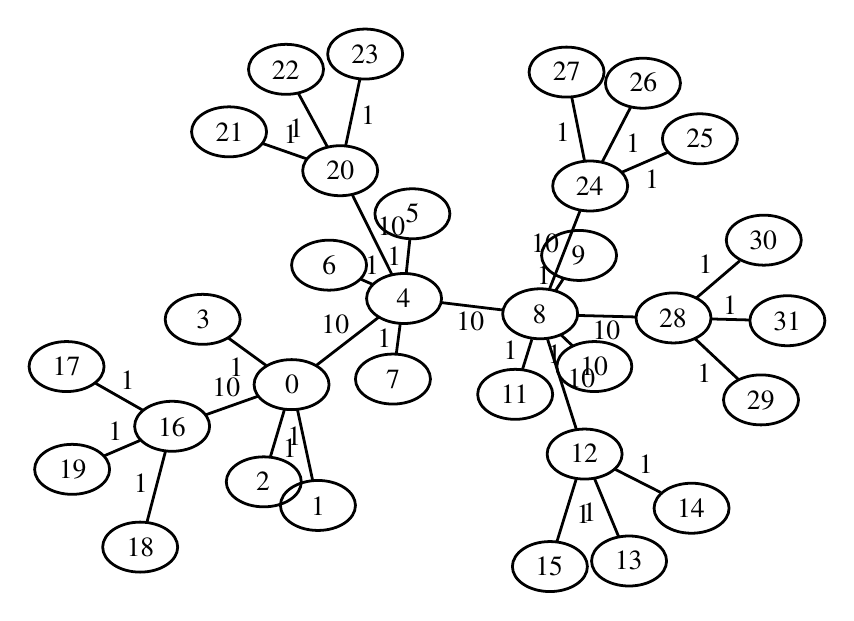
\begin{tikzpicture}[>=latex,line join=bevel,scale=.5]
  \pgfsetlinewidth{1bp}
%%
\pgfsetcolor{black}
  % Edge: 0 -- 16
  \draw [] (166.21bp,141.75bp) .. controls (154.21bp,137.5bp) and (139.75bp,132.37bp)  .. (127.78bp,128.12bp);
  \definecolor{strokecol}{rgb}{0.0,0.0,0.0};
  \pgfsetstrokecolor{strokecol}
  \draw (142.99bp,147.94bp) node {$10$};
  % Edge: 24 -- 8
  \draw [] (397.66bp,275.03bp) .. controls (391.25bp,258.58bp) and (381.78bp,234.27bp)  .. (375.41bp,217.94bp);
  \draw (372.53bp,251.48bp) node {$10$};
  % Edge: 3 -- 0
  \draw [] (144.86bp,183.29bp) .. controls (153.27bp,177.19bp) and (163.2bp,169.98bp)  .. (171.63bp,163.85bp);
  \draw (150.24bp,162.57bp) node {$1$};
  % Edge: 13 -- 12
  \draw [] (425.39bp,40.785bp) .. controls (420.15bp,53.394bp) and (413.1bp,70.342bp)  .. (407.87bp,82.936bp);
  \draw (404.63bp,57.86bp) node {$1$};
  % Edge: 28 -- 30
  \draw [] (481.35bp,212.31bp) .. controls (490.97bp,220.54bp) and (503.03bp,230.85bp)  .. (512.69bp,239.11bp);
  \draw (488.02bp,236.71bp) node {$1$};
  % Edge: 20 -- 21
  \draw [] (201.17bp,312.44bp) .. controls (191.17bp,315.94bp) and (179.56bp,319.99bp)  .. (169.53bp,323.49bp);
  \draw (189.35bp,329.97bp) node {$1$};
  % Edge: 14 -- 12
  \draw [] (455.7bp,72.393bp) .. controls (445.22bp,77.713bp) and (432.7bp,84.068bp)  .. (422.25bp,89.375bp);
  \draw (444.97bp,92.884bp) node {$1$};
  % Edge: 24 -- 25
  \draw [] (427.6bp,302.81bp) .. controls (438.25bp,307.43bp) and (450.85bp,312.89bp)  .. (461.46bp,317.49bp);
  \draw (449.53bp,298.15bp) node {$1$};
  % Edge: 23 -- 20
  \draw [] (239.16bp,369.78bp) .. controls (236.13bp,355.61bp) and (231.94bp,336.05bp)  .. (228.93bp,321.97bp);
  \draw (245.04bp,343.88bp) node {$1$};
  % Edge: 10 -- 8
  \draw [] (392.35bp,177.85bp) .. controls (389.69bp,180.39bp) and (386.93bp,183.02bp)  .. (384.27bp,185.56bp);
  \draw (379.31bp,171.71bp) node {$1$};
  % Edge: 28 -- 29
  \draw [] (480.24bp,183.31bp) .. controls (489.9bp,174.24bp) and (502.25bp,162.63bp)  .. (511.95bp,153.51bp);
  \draw (487.09bp,158.41bp) node {$1$};
  % Edge: 9 -- 8
  \draw [] (385.56bp,225.98bp) .. controls (383.61bp,223.03bp) and (381.57bp,219.97bp)  .. (379.61bp,217.03bp);
  \draw (371.59bp,228.5bp) node {$1$};
  % Edge: 26 -- 24
  \draw [] (434.35bp,350.12bp) .. controls (428.09bp,338.07bp) and (419.78bp,322.07bp)  .. (413.53bp,310.04bp);
  \draw (435.94bp,324.08bp) node {$1$};
  % Edge: 8 -- 11
  \draw [] (363.03bp,182.61bp) .. controls (360.85bp,175.62bp) and (358.35bp,167.62bp)  .. (356.17bp,160.64bp);
  \draw (347.6bp,174.63bp) node {$1$};
  % Edge: 6 -- 4
  \draw [] (239.87bp,225.9bp) .. controls (242.6bp,224.69bp) and (245.39bp,223.47bp)  .. (248.12bp,222.27bp);
  \draw (247.99bp,236.08bp) node {$1$};
  % Edge: 15 -- 12
  \draw [] (380.96bp,36.652bp) .. controls (385.14bp,50.203bp) and (390.9bp,68.839bp)  .. (395.1bp,82.452bp);
  \draw (400.03bp,56.552bp) node {$1$};
  % Edge: 20 -- 4
  \draw [] (233.67bp,286.83bp) .. controls (241.82bp,270.43bp) and (254bp,245.9bp)  .. (262.13bp,229.53bp);
  \draw (261.9bp,264.18bp) node {$10$};
  % Edge: 18 -- 16
  \draw [] (85.864bp,50.894bp) .. controls (89.75bp,65.773bp) and (95.245bp,86.812bp)  .. (99.13bp,101.68bp);
  \draw (81.497bp,79.29bp) node {$1$};
  % Edge: 27 -- 24
  \draw [] (391.64bp,357.44bp) .. controls (394.41bp,343.6bp) and (398.24bp,324.53bp)  .. (401.01bp,310.7bp);
  \draw (385.32bp,332.07bp) node {$1$};
  % Edge: 2 -- 0
  \draw [] (174.87bp,98.4bp) .. controls (178bp,108.92bp) and (181.93bp,122.13bp)  .. (185.04bp,132.6bp);
  \draw (191.95bp,112.5bp) node {$1$};
  % Edge: 28 -- 8
  \draw [] (437.62bp,198.71bp) .. controls (424.53bp,199.05bp) and (408.85bp,199.46bp)  .. (395.75bp,199.8bp);
  \draw (416.68bp,189.25bp) node {$10$};
  % Edge: 19 -- 16
  \draw [] (55.352bp,98.839bp) .. controls (63.514bp,102.34bp) and (72.694bp,106.28bp)  .. (80.851bp,109.78bp);
  \draw (63.102bp,116.31bp) node {$1$};
  % Edge: 4 -- 0
  \draw [] (252.83bp,198.58bp) .. controls (239.51bp,188.29bp) and (221.39bp,174.3bp)  .. (208.08bp,164.03bp);
  \draw (221.46bp,193.3bp) node {$10$};
  % Edge: 8 -- 12
  \draw [] (374.34bp,182.6bp) .. controls (380.17bp,164.37bp) and (389.15bp,136.27bp)  .. (394.96bp,118.1bp);
  \draw (398.65bp,154.35bp) node {$10$};
  % Edge: 20 -- 22
  \draw [] (215.78bp,321.25bp) .. controls (209.51bp,332.8bp) and (201.28bp,347.96bp)  .. (195.03bp,359.48bp);
  \draw (193.4bp,334.37bp) node {$1$};
  % Edge: 1 -- 0
  \draw [] (205.21bp,80.92bp) .. controls (201.98bp,95.938bp) and (197.42bp,117.17bp)  .. (194.19bp,132.19bp);
  \draw (188.7bp,104.55bp) node {$1$};
  % Edge: 4 -- 8
  \draw [] (297.43bp,209.11bp) .. controls (311.25bp,207.44bp) and (328.07bp,205.41bp)  .. (341.89bp,203.74bp);
  \draw (318.66bp,195.43bp) node {$10$};
  % Edge: 17 -- 16
  \draw [] (48.717bp,151.05bp) .. controls (59.414bp,144.95bp) and (72.429bp,137.53bp)  .. (83.123bp,131.43bp);
  \draw (71.92bp,153.24bp) node {$1$};
  % Edge: 4 -- 7
  \draw [] (268.29bp,194.2bp) .. controls (267.36bp,187.11bp) and (266.29bp,178.99bp)  .. (265.36bp,171.91bp);
  \draw (256.82bp,183.06bp) node {$1$};
  % Edge: 5 -- 4
  \draw [] (275.2bp,254.93bp) .. controls (274.38bp,247.23bp) and (273.43bp,238.29bp)  .. (272.61bp,230.59bp);
  \draw (263.9bp,242.76bp) node {$1$};
  % Edge: 28 -- 31
  \draw [] (492bp,197.27bp) .. controls (500.87bp,197.04bp) and (510.71bp,196.77bp)  .. (519.58bp,196.54bp);
  \draw (505.79bp,206.91bp) node {$1$};
  % Node: 24
\begin{scope}
  \definecolor{strokecol}{rgb}{0.0,0.0,0.0};
  \pgfsetstrokecolor{strokecol}
  \draw (405bp,293bp) ellipse (27bp and 18bp);
  \draw (404.59bp,292.83bp) node {$24$};
\end{scope}
  % Node: 25
\begin{scope}
  \definecolor{strokecol}{rgb}{0.0,0.0,0.0};
  \pgfsetstrokecolor{strokecol}
  \draw (484bp,327bp) ellipse (27bp and 18bp);
  \draw (484.14bp,327.33bp) node {$25$};
\end{scope}
  % Node: 26
\begin{scope}
  \definecolor{strokecol}{rgb}{0.0,0.0,0.0};
  \pgfsetstrokecolor{strokecol}
  \draw (443bp,367bp) ellipse (27bp and 18bp);
  \draw (443.33bp,367.42bp) node {$26$};
\end{scope}
  % Node: 27
\begin{scope}
  \definecolor{strokecol}{rgb}{0.0,0.0,0.0};
  \pgfsetstrokecolor{strokecol}
  \draw (388bp,375bp) ellipse (27bp and 18bp);
  \draw (388.04bp,375.34bp) node {$27$};
\end{scope}
  % Node: 20
\begin{scope}
  \definecolor{strokecol}{rgb}{0.0,0.0,0.0};
  \pgfsetstrokecolor{strokecol}
  \draw (225bp,304bp) ellipse (27bp and 18bp);
  \draw (225.1bp,304.09bp) node {$20$};
\end{scope}
  % Node: 21
\begin{scope}
  \definecolor{strokecol}{rgb}{0.0,0.0,0.0};
  \pgfsetstrokecolor{strokecol}
  \draw (145bp,332bp) ellipse (27bp and 18bp);
  \draw (145.34bp,331.94bp) node {$21$};
\end{scope}
  % Node: 22
\begin{scope}
  \definecolor{strokecol}{rgb}{0.0,0.0,0.0};
  \pgfsetstrokecolor{strokecol}
  \draw (186bp,377bp) ellipse (27bp and 18bp);
  \draw (185.78bp,376.53bp) node {$22$};
\end{scope}
  % Node: 23
\begin{scope}
  \definecolor{strokecol}{rgb}{0.0,0.0,0.0};
  \pgfsetstrokecolor{strokecol}
  \draw (243bp,388bp) ellipse (27bp and 18bp);
  \draw (243.05bp,387.99bp) node {$23$};
\end{scope}
  % Node: 28
\begin{scope}
  \definecolor{strokecol}{rgb}{0.0,0.0,0.0};
  \pgfsetstrokecolor{strokecol}
  \draw (465bp,198bp) ellipse (27bp and 18bp);
  \draw (464.62bp,198bp) node {$28$};
\end{scope}
  % Node: 29
\begin{scope}
  \definecolor{strokecol}{rgb}{0.0,0.0,0.0};
  \pgfsetstrokecolor{strokecol}
  \draw (528bp,139bp) ellipse (27bp and 18bp);
  \draw (527.83bp,138.57bp) node {$29$};
\end{scope}
  % Node: 1
\begin{scope}
  \definecolor{strokecol}{rgb}{0.0,0.0,0.0};
  \pgfsetstrokecolor{strokecol}
  \draw (209bp,63bp) ellipse (27bp and 18bp);
  \draw (209.11bp,62.79bp) node {$1$};
\end{scope}
  % Node: 0
\begin{scope}
  \definecolor{strokecol}{rgb}{0.0,0.0,0.0};
  \pgfsetstrokecolor{strokecol}
  \draw (190bp,150bp) ellipse (27bp and 18bp);
  \draw (190.3bp,150.29bp) node {$0$};
\end{scope}
  % Node: 3
\begin{scope}
  \definecolor{strokecol}{rgb}{0.0,0.0,0.0};
  \pgfsetstrokecolor{strokecol}
  \draw (126bp,197bp) ellipse (27bp and 18bp);
  \draw (126.37bp,196.72bp) node {$3$};
\end{scope}
  % Node: 2
\begin{scope}
  \definecolor{strokecol}{rgb}{0.0,0.0,0.0};
  \pgfsetstrokecolor{strokecol}
  \draw (170bp,80bp) ellipse (27bp and 18bp);
  \draw (169.52bp,80.402bp) node {$2$};
\end{scope}
  % Node: 5
\begin{scope}
  \definecolor{strokecol}{rgb}{0.0,0.0,0.0};
  \pgfsetstrokecolor{strokecol}
  \draw (277bp,273bp) ellipse (27bp and 18bp);
  \draw (277.14bp,273.19bp) node {$5$};
\end{scope}
  % Node: 4
\begin{scope}
  \definecolor{strokecol}{rgb}{0.0,0.0,0.0};
  \pgfsetstrokecolor{strokecol}
  \draw (271bp,212bp) ellipse (27bp and 18bp);
  \draw (270.67bp,212.35bp) node {$4$};
\end{scope}
  % Node: 7
\begin{scope}
  \definecolor{strokecol}{rgb}{0.0,0.0,0.0};
  \pgfsetstrokecolor{strokecol}
  \draw (263bp,154bp) ellipse (27bp and 18bp);
  \draw (263.01bp,153.98bp) node {$7$};
\end{scope}
  % Node: 6
\begin{scope}
  \definecolor{strokecol}{rgb}{0.0,0.0,0.0};
  \pgfsetstrokecolor{strokecol}
  \draw (217bp,236bp) ellipse (27bp and 18bp);
  \draw (217.18bp,235.87bp) node {$6$};
\end{scope}
  % Node: 9
\begin{scope}
  \definecolor{strokecol}{rgb}{0.0,0.0,0.0};
  \pgfsetstrokecolor{strokecol}
  \draw (397bp,243bp) ellipse (27bp and 18bp);
  \draw (396.64bp,242.62bp) node {$9$};
\end{scope}
  % Node: 8
\begin{scope}
  \definecolor{strokecol}{rgb}{0.0,0.0,0.0};
  \pgfsetstrokecolor{strokecol}
  \draw (369bp,201bp) ellipse (27bp and 18bp);
  \draw (368.62bp,200.5bp) node {$8$};
\end{scope}
  % Node: 11
\begin{scope}
  \definecolor{strokecol}{rgb}{0.0,0.0,0.0};
  \pgfsetstrokecolor{strokecol}
  \draw (351bp,143bp) ellipse (27bp and 18bp);
  \draw (350.65bp,142.96bp) node {$11$};
\end{scope}
  % Node: 10
\begin{scope}
  \definecolor{strokecol}{rgb}{0.0,0.0,0.0};
  \pgfsetstrokecolor{strokecol}
  \draw (408bp,163bp) ellipse (27bp and 18bp);
  \draw (407.85bp,163.05bp) node {$10$};
\end{scope}
  % Node: 13
\begin{scope}
  \definecolor{strokecol}{rgb}{0.0,0.0,0.0};
  \pgfsetstrokecolor{strokecol}
  \draw (433bp,23bp) ellipse (27bp and 18bp);
  \draw (432.66bp,23.301bp) node {$13$};
\end{scope}
  % Node: 12
\begin{scope}
  \definecolor{strokecol}{rgb}{0.0,0.0,0.0};
  \pgfsetstrokecolor{strokecol}
  \draw (401bp,100bp) ellipse (27bp and 18bp);
  \draw (400.63bp,100.35bp) node {$12$};
\end{scope}
  % Node: 15
\begin{scope}
  \definecolor{strokecol}{rgb}{0.0,0.0,0.0};
  \pgfsetstrokecolor{strokecol}
  \draw (376bp,19bp) ellipse (27bp and 18bp);
  \draw (375.51bp,19bp) node {$15$};
\end{scope}
  % Node: 14
\begin{scope}
  \definecolor{strokecol}{rgb}{0.0,0.0,0.0};
  \pgfsetstrokecolor{strokecol}
  \draw (478bp,61bp) ellipse (27bp and 18bp);
  \draw (477.53bp,61.31bp) node {$14$};
\end{scope}
  % Node: 17
\begin{scope}
  \definecolor{strokecol}{rgb}{0.0,0.0,0.0};
  \pgfsetstrokecolor{strokecol}
  \draw (28bp,163bp) ellipse (27bp and 18bp);
  \draw (28bp,162.87bp) node {$17$};
\end{scope}
  % Node: 16
\begin{scope}
  \definecolor{strokecol}{rgb}{0.0,0.0,0.0};
  \pgfsetstrokecolor{strokecol}
  \draw (104bp,120bp) ellipse (27bp and 18bp);
  \draw (103.82bp,119.62bp) node {$16$};
\end{scope}
  % Node: 19
\begin{scope}
  \definecolor{strokecol}{rgb}{0.0,0.0,0.0};
  \pgfsetstrokecolor{strokecol}
  \draw (32bp,89bp) ellipse (27bp and 18bp);
  \draw (32.345bp,88.971bp) node {$19$};
\end{scope}
  % Node: 18
\begin{scope}
  \definecolor{strokecol}{rgb}{0.0,0.0,0.0};
  \pgfsetstrokecolor{strokecol}
  \draw (81bp,33bp) ellipse (27bp and 18bp);
  \draw (81.173bp,32.931bp) node {$18$};
\end{scope}
  % Node: 31
\begin{scope}
  \definecolor{strokecol}{rgb}{0.0,0.0,0.0};
  \pgfsetstrokecolor{strokecol}
  \draw (547bp,196bp) ellipse (27bp and 18bp);
  \draw (546.84bp,195.81bp) node {$31$};
\end{scope}
  % Node: 30
\begin{scope}
  \definecolor{strokecol}{rgb}{0.0,0.0,0.0};
  \pgfsetstrokecolor{strokecol}
  \draw (530bp,254bp) ellipse (27bp and 18bp);
  \draw (529.59bp,253.56bp) node {$30$};
\end{scope}
%

\end{tikzpicture}
\caption{Multicast tree automatically found for a 8x4x1 multicore}
\label{fig:mst_gruyere}
\end{figure}

%-------------------------------------------------
\subsubsection{Hierarchical}

We now consider NUMA node for coming up with a broadcast tree. We
select one coordinator node in every node and build a binary tree
for the coordinators. We call this topology connecting nodes across
NUMA domains the \emph{outer} network.

Each coordinator is also responsible for sending a message to all
other cores of the node. We currently do this sequentially, since the
number of cores in a node is typically very small. Alternatively, a
binary tree could be used as well. We call overlay networks within
NUMA nodes \emph{inner} networks.

We show an example hierarchical tree in
Figure~\ref{fig:gruyere_hierarchy}.

\begin{figure}
\begin{tikzpicture}[>=latex,line join=bevel,scale=.5]
  \pgfsetlinewidth{.5bp}
\input{graphs/final_gruyere_hierarchical}
\end{tikzpicture}
\caption{Hierarchical tree for a 8x4x1 multicore. Nodes 0, 4, 8, 12,
  16, 20, 24 and 28 are coordinators. They are arranged in a binary
  tree starting at node 0. Communication within NUMA nodes is
  sequential (as an example: coordinator node 24 sends a message to
  all cores on the same NUMA node, namely 25, 26 and 27)}
\label{fig:gruyere_hierarchy}
\end{figure}


%-------------------------------------------------
\subsubsection{Clustering}

\stefan{Have not implemented this, but it might be interesting to try
  out later}

We discussed earlier in Section~\ref{sec:model} that
multicore machines are hierarchical.%

We divide the space into clusters. In every round, we further split up
all cluster into smaller clusters and connect them with the minimal
link. 

We find this link by searching for links that have start and
end node in different regions of the most recent split. Out of these
links, we pick the cheapest ones. We ignore links whose start or end
node have a too high degree in the spanning tree already.

Assuming that the choice of node IDs represents the topology to some
extend, splitting them up into distinct clusters avoids contention, as
two separate sub-trees are processed in different areas of the
interconnect network.

Another idea is to employ clustering on NUMA domains such that every
NUMA domain corresponds to one cluster. 

%%%%%%%%%%%%%%%%%%%%%%%%%%%%%%%%%%%%%%%%%%%%%%%%%%
\subsection{Ring topology}

Next, we evaluate ring topologies. Rings experience a certain level of
redundancy. The sending node receives the node back on the ring. This
is unnecessary for applications with uni-directional traffic executed
on reliable communication channels

For applications that require some form of feedback (as well as
unreliable channels, which we do not consider at this point), rings
have the advantage that they can piggy-back some information that will
eventually arrive back on the sender. This is beneficial for some
algorithms such as quorums, where nodes report the result of the
quorum back to the sender.

The downside is that some state is required on every node to remember
whether or not a message was received before. If messages are just
forwarded as they arrive, message transport does never terminate.

To add more parallelism, we add a second ring, which we send the
message on in parallel. Acknowledgments, however, only work if
forwarding along the ring is only done after all local nodes (as in
nodes from the outer rings) acknowledge a message. In
Figure~\ref{fig:gruyere_ring}, we visualize an example of two
intertwined ring topologies. Node that the link from node 20 to 8 is a
two hop link and, thus, has a cost of 20 instead of the usual 10.

\begin{figure}
\begin{tikzpicture}[>=latex,line join=bevel,scale=.5]
  \pgfsetlinewidth{.5bp}
\input{graphs/final_ring}
\end{tikzpicture}
\caption{Outer overlay as ring with sequential inner overlay for a
  8x4x1 multicore}
\label{fig:gruyere_ring}
\end{figure}

%%%%%%%%%%%%%%%%%%%%%%%%%%%%%%%%%%%%%%%%%%%%%%%%%%
%%%%%%%%%%%%%%%%%%%%%%%%%%%%%%%%%%%%%%%%%%%%%%%%%%
\section{Scheduling}
\label{sec:scheduling}

% Tree -> scheduling
Assuming the tree (or some other kind of overlay network), there is a
\emph{scheduling problems} for the order in which to send messages to
children. The intuition is to send on long-delay links first to hide
the more expensive latencies, as this link is dominating total send
cost.

In Figure~\ref{fig:mst_gruyere_operations}, we visualize sending of a
broadcast message in \naive order. We use the MST given in
Figure~\ref{fig:mst_gruyere}.  When core 08 sends its six messages, it
does so in random order (here: in increasing node ID order). This is
inefficient, as the latency of the broadcast is dominated by cores 12,
24 and 28 rather than cores 9, 10 and 11.

\begin{figure}[htb]
  \centering
  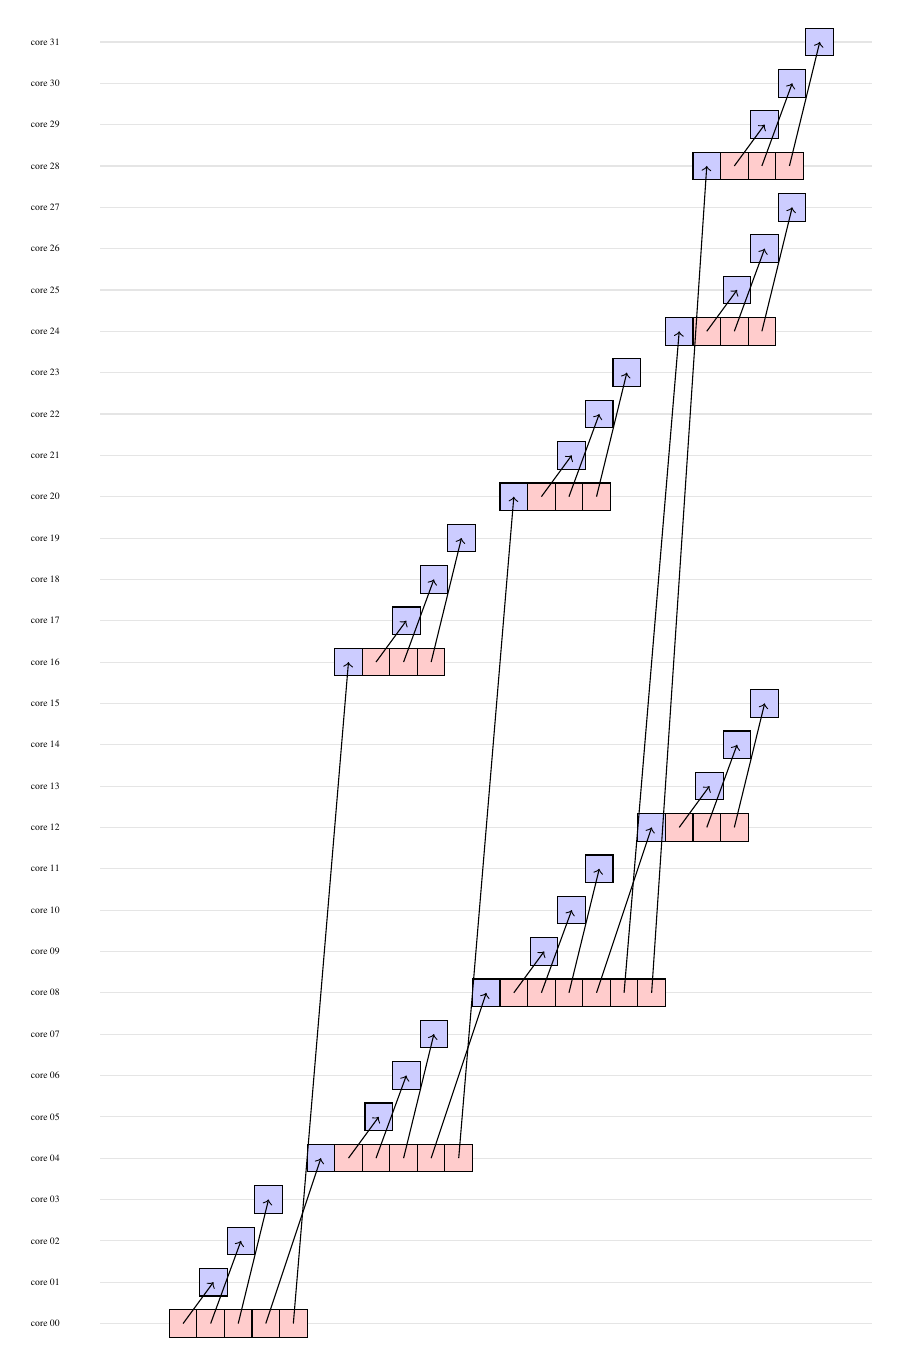
\begin{tikzpicture}[scale=.35,transform shape]
    % Insert visualization
    \node at (0mm,0mm) {core 00};
\draw[color=black!10] (20mm,0mm) -- (30cm,0mm);
\node at (0mm,15mm) {core 01};
\draw[color=black!10] (20mm,15mm) -- (30cm,15mm);
\node at (0mm,30mm) {core 02};
\draw[color=black!10] (20mm,30mm) -- (30cm,30mm);
\node at (0mm,45mm) {core 03};
\draw[color=black!10] (20mm,45mm) -- (30cm,45mm);
\node at (0mm,60mm) {core 04};
\draw[color=black!10] (20mm,60mm) -- (30cm,60mm);
\node at (0mm,75mm) {core 05};
\draw[color=black!10] (20mm,75mm) -- (30cm,75mm);
\node at (0mm,90mm) {core 06};
\draw[color=black!10] (20mm,90mm) -- (30cm,90mm);
\node at (0mm,105mm) {core 07};
\draw[color=black!10] (20mm,105mm) -- (30cm,105mm);
\node at (0mm,120mm) {core 08};
\draw[color=black!10] (20mm,120mm) -- (30cm,120mm);
\node at (0mm,135mm) {core 09};
\draw[color=black!10] (20mm,135mm) -- (30cm,135mm);
\node at (0mm,150mm) {core 10};
\draw[color=black!10] (20mm,150mm) -- (30cm,150mm);
\node at (0mm,165mm) {core 11};
\draw[color=black!10] (20mm,165mm) -- (30cm,165mm);
\node at (0mm,180mm) {core 12};
\draw[color=black!10] (20mm,180mm) -- (30cm,180mm);
\node at (0mm,195mm) {core 13};
\draw[color=black!10] (20mm,195mm) -- (30cm,195mm);
\node at (0mm,210mm) {core 14};
\draw[color=black!10] (20mm,210mm) -- (30cm,210mm);
\node at (0mm,225mm) {core 15};
\draw[color=black!10] (20mm,225mm) -- (30cm,225mm);
\node at (0mm,240mm) {core 16};
\draw[color=black!10] (20mm,240mm) -- (30cm,240mm);
\node at (0mm,255mm) {core 17};
\draw[color=black!10] (20mm,255mm) -- (30cm,255mm);
\node at (0mm,270mm) {core 18};
\draw[color=black!10] (20mm,270mm) -- (30cm,270mm);
\node at (0mm,285mm) {core 19};
\draw[color=black!10] (20mm,285mm) -- (30cm,285mm);
\node at (0mm,300mm) {core 20};
\draw[color=black!10] (20mm,300mm) -- (30cm,300mm);
\node at (0mm,315mm) {core 21};
\draw[color=black!10] (20mm,315mm) -- (30cm,315mm);
\node at (0mm,330mm) {core 22};
\draw[color=black!10] (20mm,330mm) -- (30cm,330mm);
\node at (0mm,345mm) {core 23};
\draw[color=black!10] (20mm,345mm) -- (30cm,345mm);
\node at (0mm,360mm) {core 24};
\draw[color=black!10] (20mm,360mm) -- (30cm,360mm);
\node at (0mm,375mm) {core 25};
\draw[color=black!10] (20mm,375mm) -- (30cm,375mm);
\node at (0mm,390mm) {core 26};
\draw[color=black!10] (20mm,390mm) -- (30cm,390mm);
\node at (0mm,405mm) {core 27};
\draw[color=black!10] (20mm,405mm) -- (30cm,405mm);
\node at (0mm,420mm) {core 28};
\draw[color=black!10] (20mm,420mm) -- (30cm,420mm);
\node at (0mm,435mm) {core 29};
\draw[color=black!10] (20mm,435mm) -- (30cm,435mm);
\node at (0mm,450mm) {core 30};
\draw[color=black!10] (20mm,450mm) -- (30cm,450mm);
\node at (0mm,465mm) {core 31};
\draw[color=black!10] (20mm,465mm) -- (30cm,465mm);
\node[draw,fill=red!20,minimum size=10mm] (s_0_1) at (50mm,0mm) {};
\node[draw,fill=red!20,minimum size=10mm] (s_0_2) at (60mm,0mm) {};
\node[draw,fill=red!20,minimum size=10mm] (s_0_3) at (70mm,0mm) {};
\node[draw,fill=red!20,minimum size=10mm] (s_0_4) at (80mm,0mm) {};
\node[draw,fill=red!20,minimum size=10mm] (s_0_16) at (90mm,0mm) {};
\node[draw,fill=blue!20,minimum size=10mm] (r_0_1) at (61mm,15mm) {};
\draw[->] (s_0_1.center) -- (r_0_1.center); 
\node[draw,fill=blue!20,minimum size=10mm] (r_0_2) at (71mm,30mm) {};
\draw[->] (s_0_2.center) -- (r_0_2.center); 
\node[draw,fill=blue!20,minimum size=10mm] (r_0_3) at (81mm,45mm) {};
\draw[->] (s_0_3.center) -- (r_0_3.center); 
\node[draw,fill=blue!20,minimum size=10mm] (r_0_4) at (100mm,60mm) {};
\draw[->] (s_0_4.center) -- (r_0_4.center); 
\node[draw,fill=red!20,minimum size=10mm] (s_4_5) at (110mm,60mm) {};
\node[draw,fill=red!20,minimum size=10mm] (s_4_6) at (120mm,60mm) {};
\node[draw,fill=red!20,minimum size=10mm] (s_4_7) at (130mm,60mm) {};
\node[draw,fill=red!20,minimum size=10mm] (s_4_8) at (140mm,60mm) {};
\node[draw,fill=red!20,minimum size=10mm] (s_4_20) at (150mm,60mm) {};
\node[draw,fill=blue!20,minimum size=10mm] (r_0_16) at (110mm,240mm) {};
\draw[->] (s_0_16.center) -- (r_0_16.center); 
\node[draw,fill=red!20,minimum size=10mm] (s_16_17) at (120mm,240mm) {};
\node[draw,fill=red!20,minimum size=10mm] (s_16_18) at (130mm,240mm) {};
\node[draw,fill=red!20,minimum size=10mm] (s_16_19) at (140mm,240mm) {};
\node[draw,fill=blue!20,minimum size=10mm] (r_4_5) at (121mm,75mm) {};
\draw[->] (s_4_5.center) -- (r_4_5.center); 
\node[draw,fill=blue!20,minimum size=10mm] (r_16_17) at (131mm,255mm) {};
\draw[->] (s_16_17.center) -- (r_16_17.center); 
\node[draw,fill=blue!20,minimum size=10mm] (r_4_6) at (131mm,90mm) {};
\draw[->] (s_4_6.center) -- (r_4_6.center); 
\node[draw,fill=blue!20,minimum size=10mm] (r_16_18) at (141mm,270mm) {};
\draw[->] (s_16_18.center) -- (r_16_18.center); 
\node[draw,fill=blue!20,minimum size=10mm] (r_4_7) at (141mm,105mm) {};
\draw[->] (s_4_7.center) -- (r_4_7.center); 
\node[draw,fill=blue!20,minimum size=10mm] (r_16_19) at (151mm,285mm) {};
\draw[->] (s_16_19.center) -- (r_16_19.center); 
\node[draw,fill=blue!20,minimum size=10mm] (r_4_8) at (160mm,120mm) {};
\draw[->] (s_4_8.center) -- (r_4_8.center); 
\node[draw,fill=red!20,minimum size=10mm] (s_8_9) at (170mm,120mm) {};
\node[draw,fill=red!20,minimum size=10mm] (s_8_10) at (180mm,120mm) {};
\node[draw,fill=red!20,minimum size=10mm] (s_8_11) at (190mm,120mm) {};
\node[draw,fill=red!20,minimum size=10mm] (s_8_12) at (200mm,120mm) {};
\node[draw,fill=red!20,minimum size=10mm] (s_8_24) at (210mm,120mm) {};
\node[draw,fill=red!20,minimum size=10mm] (s_8_28) at (220mm,120mm) {};
\node[draw,fill=blue!20,minimum size=10mm] (r_4_20) at (170mm,300mm) {};
\draw[->] (s_4_20.center) -- (r_4_20.center); 
\node[draw,fill=red!20,minimum size=10mm] (s_20_21) at (180mm,300mm) {};
\node[draw,fill=red!20,minimum size=10mm] (s_20_22) at (190mm,300mm) {};
\node[draw,fill=red!20,minimum size=10mm] (s_20_23) at (200mm,300mm) {};
\node[draw,fill=blue!20,minimum size=10mm] (r_8_9) at (181mm,135mm) {};
\draw[->] (s_8_9.center) -- (r_8_9.center); 
\node[draw,fill=blue!20,minimum size=10mm] (r_20_21) at (191mm,315mm) {};
\draw[->] (s_20_21.center) -- (r_20_21.center); 
\node[draw,fill=blue!20,minimum size=10mm] (r_8_10) at (191mm,150mm) {};
\draw[->] (s_8_10.center) -- (r_8_10.center); 
\node[draw,fill=blue!20,minimum size=10mm] (r_20_22) at (201mm,330mm) {};
\draw[->] (s_20_22.center) -- (r_20_22.center); 
\node[draw,fill=blue!20,minimum size=10mm] (r_8_11) at (201mm,165mm) {};
\draw[->] (s_8_11.center) -- (r_8_11.center); 
\node[draw,fill=blue!20,minimum size=10mm] (r_20_23) at (211mm,345mm) {};
\draw[->] (s_20_23.center) -- (r_20_23.center); 
\node[draw,fill=blue!20,minimum size=10mm] (r_8_12) at (220mm,180mm) {};
\draw[->] (s_8_12.center) -- (r_8_12.center); 
\node[draw,fill=red!20,minimum size=10mm] (s_12_13) at (230mm,180mm) {};
\node[draw,fill=red!20,minimum size=10mm] (s_12_14) at (240mm,180mm) {};
\node[draw,fill=red!20,minimum size=10mm] (s_12_15) at (250mm,180mm) {};
\node[draw,fill=blue!20,minimum size=10mm] (r_8_24) at (230mm,360mm) {};
\draw[->] (s_8_24.center) -- (r_8_24.center); 
\node[draw,fill=red!20,minimum size=10mm] (s_24_25) at (240mm,360mm) {};
\node[draw,fill=red!20,minimum size=10mm] (s_24_26) at (250mm,360mm) {};
\node[draw,fill=red!20,minimum size=10mm] (s_24_27) at (260mm,360mm) {};
\node[draw,fill=blue!20,minimum size=10mm] (r_8_28) at (240mm,420mm) {};
\draw[->] (s_8_28.center) -- (r_8_28.center); 
\node[draw,fill=red!20,minimum size=10mm] (s_28_29) at (250mm,420mm) {};
\node[draw,fill=red!20,minimum size=10mm] (s_28_30) at (260mm,420mm) {};
\node[draw,fill=red!20,minimum size=10mm] (s_28_31) at (270mm,420mm) {};
\node[draw,fill=blue!20,minimum size=10mm] (r_12_13) at (241mm,195mm) {};
\draw[->] (s_12_13.center) -- (r_12_13.center); 
\node[draw,fill=blue!20,minimum size=10mm] (r_12_14) at (251mm,210mm) {};
\draw[->] (s_12_14.center) -- (r_12_14.center); 
\node[draw,fill=blue!20,minimum size=10mm] (r_24_25) at (251mm,375mm) {};
\draw[->] (s_24_25.center) -- (r_24_25.center); 
\node[draw,fill=blue!20,minimum size=10mm] (r_28_29) at (261mm,435mm) {};
\draw[->] (s_28_29.center) -- (r_28_29.center); 
\node[draw,fill=blue!20,minimum size=10mm] (r_24_26) at (261mm,390mm) {};
\draw[->] (s_24_26.center) -- (r_24_26.center); 
\node[draw,fill=blue!20,minimum size=10mm] (r_12_15) at (261mm,225mm) {};
\draw[->] (s_12_15.center) -- (r_12_15.center); 
\node[draw,fill=blue!20,minimum size=10mm] (r_28_30) at (271mm,450mm) {};
\draw[->] (s_28_30.center) -- (r_28_30.center); 
\node[draw,fill=blue!20,minimum size=10mm] (r_24_27) at (271mm,405mm) {};
\draw[->] (s_24_27.center) -- (r_24_27.center); 
\node[draw,fill=blue!20,minimum size=10mm] (r_28_31) at (281mm,465mm) {};
\draw[->] (s_28_31.center) -- (r_28_31.center); 

  \end{tikzpicture}
  \caption{Visualization of operations for sending a message along the
    tree. Red boxes represent send operations, blue boxes represent
    receive operations and arrows messages sent between cores. The
    tree has been acquired using an MST algorithm.}
  \label{fig:mst_gruyere_operations}
\end{figure}

In Figure~\ref{fig:mst_gruyere_operations_sorted} we schedule sending
of messages based on link cost. We sort the outgoing edges by their
weights and send on the most expensive links first. See
Algorithm~\ref{algo:scheduling_link_weight}

\begin{algorithm}[htb]
\SetCommentSty{textc}
\SetKwFunction{weight}{edge\_weight}%
\SetKwFunction{sort}{sort\_by\_edge\_weight}%
\SetKwFunction{icsend}{send}%
  %
  \KwData{Node $n$ sending messages, \\ %
    broadcast tree as graph $(V, E)$, \\ %
    weight function \weight{$E$}
    %
  }
  % 
  \BlankLine
  $nb \leftarrow \{ c: \exists (self, c) \in E \}$\tcp*{Get children}
  $nb \leftarrow $ \sort{$nb$, \weight{}}\tcp*{Sort by edge weight}
  \For(\tcp*{For all children}){$c \leftarrow nb$}{
    \icsend{$c$}
  }
  % 
  \caption{Scheduling in order of outgoing link weight}
  \label{algo:scheduling_link_weight}
\end{algorithm}

\begin{figure}[htb]
  \centering
  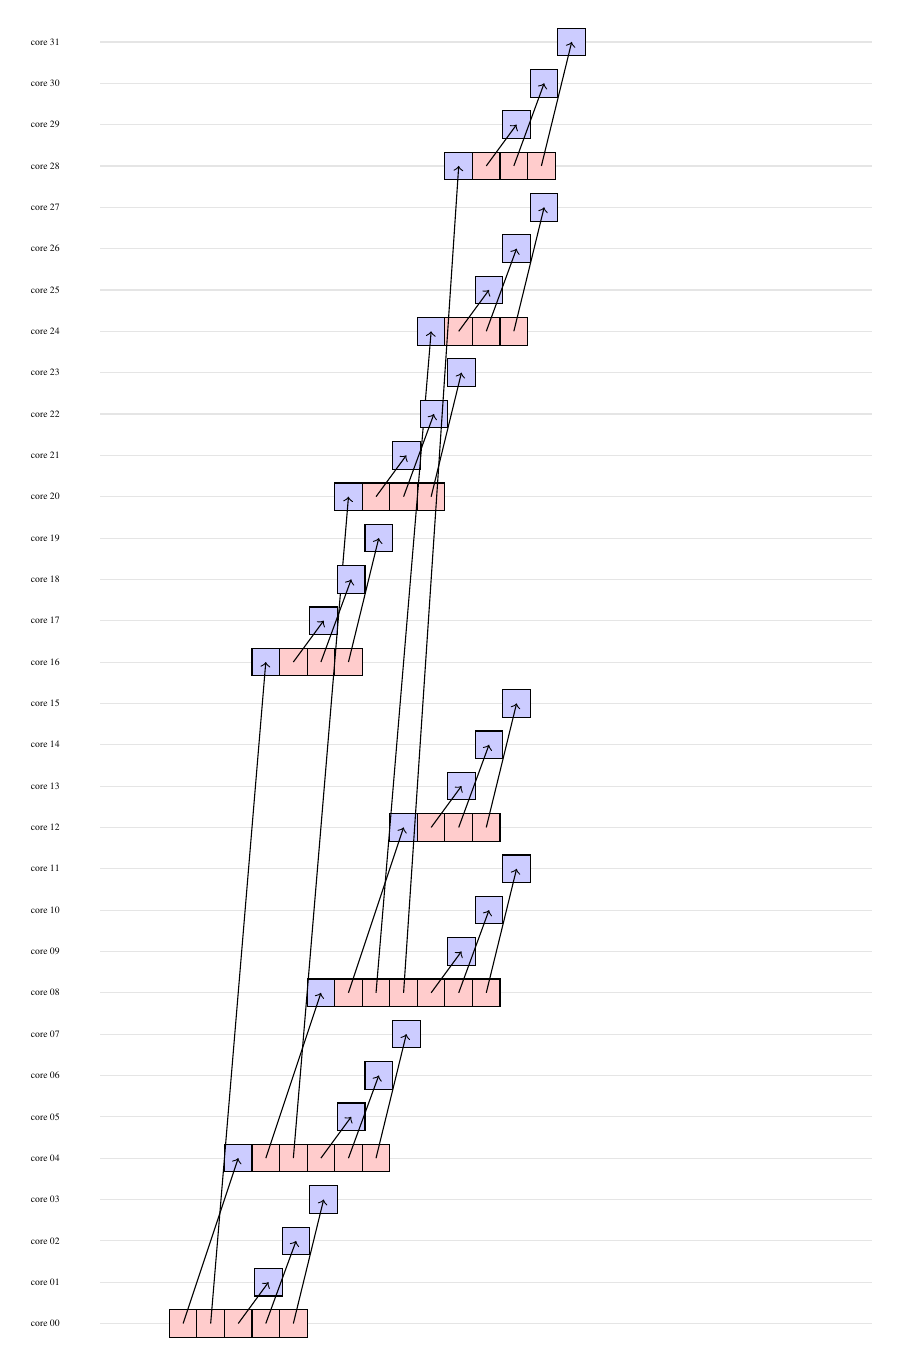
\begin{tikzpicture}[scale=.35,transform shape]
    % Insert visualization
    \node at (0mm,0mm) {core 00};
\draw[color=black!10] (20mm,0mm) -- (30cm,0mm);
\node at (0mm,15mm) {core 01};
\draw[color=black!10] (20mm,15mm) -- (30cm,15mm);
\node at (0mm,30mm) {core 02};
\draw[color=black!10] (20mm,30mm) -- (30cm,30mm);
\node at (0mm,45mm) {core 03};
\draw[color=black!10] (20mm,45mm) -- (30cm,45mm);
\node at (0mm,60mm) {core 04};
\draw[color=black!10] (20mm,60mm) -- (30cm,60mm);
\node at (0mm,75mm) {core 05};
\draw[color=black!10] (20mm,75mm) -- (30cm,75mm);
\node at (0mm,90mm) {core 06};
\draw[color=black!10] (20mm,90mm) -- (30cm,90mm);
\node at (0mm,105mm) {core 07};
\draw[color=black!10] (20mm,105mm) -- (30cm,105mm);
\node at (0mm,120mm) {core 08};
\draw[color=black!10] (20mm,120mm) -- (30cm,120mm);
\node at (0mm,135mm) {core 09};
\draw[color=black!10] (20mm,135mm) -- (30cm,135mm);
\node at (0mm,150mm) {core 10};
\draw[color=black!10] (20mm,150mm) -- (30cm,150mm);
\node at (0mm,165mm) {core 11};
\draw[color=black!10] (20mm,165mm) -- (30cm,165mm);
\node at (0mm,180mm) {core 12};
\draw[color=black!10] (20mm,180mm) -- (30cm,180mm);
\node at (0mm,195mm) {core 13};
\draw[color=black!10] (20mm,195mm) -- (30cm,195mm);
\node at (0mm,210mm) {core 14};
\draw[color=black!10] (20mm,210mm) -- (30cm,210mm);
\node at (0mm,225mm) {core 15};
\draw[color=black!10] (20mm,225mm) -- (30cm,225mm);
\node at (0mm,240mm) {core 16};
\draw[color=black!10] (20mm,240mm) -- (30cm,240mm);
\node at (0mm,255mm) {core 17};
\draw[color=black!10] (20mm,255mm) -- (30cm,255mm);
\node at (0mm,270mm) {core 18};
\draw[color=black!10] (20mm,270mm) -- (30cm,270mm);
\node at (0mm,285mm) {core 19};
\draw[color=black!10] (20mm,285mm) -- (30cm,285mm);
\node at (0mm,300mm) {core 20};
\draw[color=black!10] (20mm,300mm) -- (30cm,300mm);
\node at (0mm,315mm) {core 21};
\draw[color=black!10] (20mm,315mm) -- (30cm,315mm);
\node at (0mm,330mm) {core 22};
\draw[color=black!10] (20mm,330mm) -- (30cm,330mm);
\node at (0mm,345mm) {core 23};
\draw[color=black!10] (20mm,345mm) -- (30cm,345mm);
\node at (0mm,360mm) {core 24};
\draw[color=black!10] (20mm,360mm) -- (30cm,360mm);
\node at (0mm,375mm) {core 25};
\draw[color=black!10] (20mm,375mm) -- (30cm,375mm);
\node at (0mm,390mm) {core 26};
\draw[color=black!10] (20mm,390mm) -- (30cm,390mm);
\node at (0mm,405mm) {core 27};
\draw[color=black!10] (20mm,405mm) -- (30cm,405mm);
\node at (0mm,420mm) {core 28};
\draw[color=black!10] (20mm,420mm) -- (30cm,420mm);
\node at (0mm,435mm) {core 29};
\draw[color=black!10] (20mm,435mm) -- (30cm,435mm);
\node at (0mm,450mm) {core 30};
\draw[color=black!10] (20mm,450mm) -- (30cm,450mm);
\node at (0mm,465mm) {core 31};
\draw[color=black!10] (20mm,465mm) -- (30cm,465mm);
\node[draw,fill=red!20,minimum size=10mm] (s_0_4) at (50mm,0mm) {};
\node[draw,fill=red!20,minimum size=10mm] (s_0_16) at (60mm,0mm) {};
\node[draw,fill=red!20,minimum size=10mm] (s_0_1) at (70mm,0mm) {};
\node[draw,fill=red!20,minimum size=10mm] (s_0_2) at (80mm,0mm) {};
\node[draw,fill=red!20,minimum size=10mm] (s_0_3) at (90mm,0mm) {};
\node[draw,fill=blue!20,minimum size=10mm] (r_0_4) at (70mm,60mm) {};
\draw[->] (s_0_4.center) -- (r_0_4.center); 
\node[draw,fill=red!20,minimum size=10mm] (s_4_8) at (80mm,60mm) {};
\node[draw,fill=red!20,minimum size=10mm] (s_4_20) at (90mm,60mm) {};
\node[draw,fill=red!20,minimum size=10mm] (s_4_5) at (100mm,60mm) {};
\node[draw,fill=red!20,minimum size=10mm] (s_4_6) at (110mm,60mm) {};
\node[draw,fill=red!20,minimum size=10mm] (s_4_7) at (120mm,60mm) {};
\node[draw,fill=blue!20,minimum size=10mm] (r_0_16) at (80mm,240mm) {};
\draw[->] (s_0_16.center) -- (r_0_16.center); 
\node[draw,fill=red!20,minimum size=10mm] (s_16_17) at (90mm,240mm) {};
\node[draw,fill=red!20,minimum size=10mm] (s_16_18) at (100mm,240mm) {};
\node[draw,fill=red!20,minimum size=10mm] (s_16_19) at (110mm,240mm) {};
\node[draw,fill=blue!20,minimum size=10mm] (r_0_1) at (81mm,15mm) {};
\draw[->] (s_0_1.center) -- (r_0_1.center); 
\node[draw,fill=blue!20,minimum size=10mm] (r_0_2) at (91mm,30mm) {};
\draw[->] (s_0_2.center) -- (r_0_2.center); 
\node[draw,fill=blue!20,minimum size=10mm] (r_4_8) at (100mm,120mm) {};
\draw[->] (s_4_8.center) -- (r_4_8.center); 
\node[draw,fill=red!20,minimum size=10mm] (s_8_12) at (110mm,120mm) {};
\node[draw,fill=red!20,minimum size=10mm] (s_8_24) at (120mm,120mm) {};
\node[draw,fill=red!20,minimum size=10mm] (s_8_28) at (130mm,120mm) {};
\node[draw,fill=red!20,minimum size=10mm] (s_8_9) at (140mm,120mm) {};
\node[draw,fill=red!20,minimum size=10mm] (s_8_10) at (150mm,120mm) {};
\node[draw,fill=red!20,minimum size=10mm] (s_8_11) at (160mm,120mm) {};
\node[draw,fill=blue!20,minimum size=10mm] (r_0_3) at (101mm,45mm) {};
\draw[->] (s_0_3.center) -- (r_0_3.center); 
\node[draw,fill=blue!20,minimum size=10mm] (r_16_17) at (101mm,255mm) {};
\draw[->] (s_16_17.center) -- (r_16_17.center); 
\node[draw,fill=blue!20,minimum size=10mm] (r_4_20) at (110mm,300mm) {};
\draw[->] (s_4_20.center) -- (r_4_20.center); 
\node[draw,fill=red!20,minimum size=10mm] (s_20_21) at (120mm,300mm) {};
\node[draw,fill=red!20,minimum size=10mm] (s_20_22) at (130mm,300mm) {};
\node[draw,fill=red!20,minimum size=10mm] (s_20_23) at (140mm,300mm) {};
\node[draw,fill=blue!20,minimum size=10mm] (r_4_5) at (111mm,75mm) {};
\draw[->] (s_4_5.center) -- (r_4_5.center); 
\node[draw,fill=blue!20,minimum size=10mm] (r_16_18) at (111mm,270mm) {};
\draw[->] (s_16_18.center) -- (r_16_18.center); 
\node[draw,fill=blue!20,minimum size=10mm] (r_4_6) at (121mm,90mm) {};
\draw[->] (s_4_6.center) -- (r_4_6.center); 
\node[draw,fill=blue!20,minimum size=10mm] (r_16_19) at (121mm,285mm) {};
\draw[->] (s_16_19.center) -- (r_16_19.center); 
\node[draw,fill=blue!20,minimum size=10mm] (r_8_12) at (130mm,180mm) {};
\draw[->] (s_8_12.center) -- (r_8_12.center); 
\node[draw,fill=red!20,minimum size=10mm] (s_12_13) at (140mm,180mm) {};
\node[draw,fill=red!20,minimum size=10mm] (s_12_14) at (150mm,180mm) {};
\node[draw,fill=red!20,minimum size=10mm] (s_12_15) at (160mm,180mm) {};
\node[draw,fill=blue!20,minimum size=10mm] (r_20_21) at (131mm,315mm) {};
\draw[->] (s_20_21.center) -- (r_20_21.center); 
\node[draw,fill=blue!20,minimum size=10mm] (r_4_7) at (131mm,105mm) {};
\draw[->] (s_4_7.center) -- (r_4_7.center); 
\node[draw,fill=blue!20,minimum size=10mm] (r_8_24) at (140mm,360mm) {};
\draw[->] (s_8_24.center) -- (r_8_24.center); 
\node[draw,fill=red!20,minimum size=10mm] (s_24_25) at (150mm,360mm) {};
\node[draw,fill=red!20,minimum size=10mm] (s_24_26) at (160mm,360mm) {};
\node[draw,fill=red!20,minimum size=10mm] (s_24_27) at (170mm,360mm) {};
\node[draw,fill=blue!20,minimum size=10mm] (r_20_22) at (141mm,330mm) {};
\draw[->] (s_20_22.center) -- (r_20_22.center); 
\node[draw,fill=blue!20,minimum size=10mm] (r_8_28) at (150mm,420mm) {};
\draw[->] (s_8_28.center) -- (r_8_28.center); 
\node[draw,fill=red!20,minimum size=10mm] (s_28_29) at (160mm,420mm) {};
\node[draw,fill=red!20,minimum size=10mm] (s_28_30) at (170mm,420mm) {};
\node[draw,fill=red!20,minimum size=10mm] (s_28_31) at (180mm,420mm) {};
\node[draw,fill=blue!20,minimum size=10mm] (r_20_23) at (151mm,345mm) {};
\draw[->] (s_20_23.center) -- (r_20_23.center); 
\node[draw,fill=blue!20,minimum size=10mm] (r_12_13) at (151mm,195mm) {};
\draw[->] (s_12_13.center) -- (r_12_13.center); 
\node[draw,fill=blue!20,minimum size=10mm] (r_8_9) at (151mm,135mm) {};
\draw[->] (s_8_9.center) -- (r_8_9.center); 
\node[draw,fill=blue!20,minimum size=10mm] (r_12_14) at (161mm,210mm) {};
\draw[->] (s_12_14.center) -- (r_12_14.center); 
\node[draw,fill=blue!20,minimum size=10mm] (r_8_10) at (161mm,150mm) {};
\draw[->] (s_8_10.center) -- (r_8_10.center); 
\node[draw,fill=blue!20,minimum size=10mm] (r_24_25) at (161mm,375mm) {};
\draw[->] (s_24_25.center) -- (r_24_25.center); 
\node[draw,fill=blue!20,minimum size=10mm] (r_28_29) at (171mm,435mm) {};
\draw[->] (s_28_29.center) -- (r_28_29.center); 
\node[draw,fill=blue!20,minimum size=10mm] (r_12_15) at (171mm,225mm) {};
\draw[->] (s_12_15.center) -- (r_12_15.center); 
\node[draw,fill=blue!20,minimum size=10mm] (r_24_26) at (171mm,390mm) {};
\draw[->] (s_24_26.center) -- (r_24_26.center); 
\node[draw,fill=blue!20,minimum size=10mm] (r_8_11) at (171mm,165mm) {};
\draw[->] (s_8_11.center) -- (r_8_11.center); 
\node[draw,fill=blue!20,minimum size=10mm] (r_28_30) at (181mm,450mm) {};
\draw[->] (s_28_30.center) -- (r_28_30.center); 
\node[draw,fill=blue!20,minimum size=10mm] (r_24_27) at (181mm,405mm) {};
\draw[->] (s_24_27.center) -- (r_24_27.center); 
\node[draw,fill=blue!20,minimum size=10mm] (r_28_31) at (191mm,465mm) {};
\draw[->] (s_28_31.center) -- (r_28_31.center); 

  \end{tikzpicture}
  \caption{Visualization of operations for sending a message along the
    tree. Red boxes represent send operations, blue boxes represent
    receive operations and arrows messages sent between cores. After
    running the MST algorithm, we optimize scheduling in every node to
    send messages in decreasing order of their latency.}
  \label{fig:mst_gruyere_operations_sorted}
\end{figure}

A better schedule for sending messages to the children of core 8 would
be to start with the child from which the longest path emerges.

\stefan{TODO: write down algorithm}

%%%%%%%%%%%%%%%%%%%%%%%%%%%%%%%%%%%%%%%%%%%%%%%%%%
\section{Implementation}
\label{sec:implementation}

% Our implementation
Assuming the tree, we now implement an atomic broadcast for multicore
machines. Our implementation is based on the Barrelfish UMP
interconnect driver. It provides reliable channels with in-order
delivery. Flow control is build in for reliability. Communication
starts at the root node, which acts as a
sequentializer. See~\ref{algo:ab} for details.

\begin{algorithm}[htb]
\SetCommentSty{textc}
\SetKwInOut{Assumptions}{assumptions}
\Assumptions{Underlying communication channel is reliable and in-order}
\SetKwProg{Fn}{Function}{}{end}%
\SetKwFunction{receive}{on\_receive}%
\SetKwFunction{waitchild}{wait\_for\_children}%
\SetKwFunction{send}{send}%
\SetKwFunction{icsend}{send\_bc\_request}%
\SetKwFunction{icsendack}{send\_bc\_ack}%
\SetKwFunction{handlemessages}{handle\_other\_messages}%
  %
  \KwData{List of processes $p$, broadcast tree as graph $(V, E)$}
  \KwResult{Tree based atomic broadcast using a sequentializer}
  % 
  \BlankLine
  \Fn(\tcp*{Receive a message}){\receive{$client$, $m$}}{
    \For(\tcp*{For all children}){$c \leftarrow \{ c: \exists (self, c) \in E \} $}{
      \icsend{c}
    }
    \waitchild{}\;
    \icsendack{$client$}\;
  }
  % 
  \BlankLine
  \Fn(\tcp*{Send a message}){\send{void}}{
    \tcc{Need to wait for acknowledgment before returning to
      caller. Otherwise, sender might see his own request before some
      other request, that the sequentializer decided to handle first}
    \icsend{$V_{root}$}\tcp*{Relay msg (sequentializer)}
    \While{no answer received}{
      \handlemessages{}\tcp*{Otherwise, deadlocks}
    }
  }
  \caption{Atomic broadcast on reliable communication channels}
  \label{algo:ab}

\end{algorithm}

%%%%%%%%%%%%%%%%%%%%%%%%%%%%%%%%%%%%%%%%%%%%%%%%%%
\subsection{Issues with the Barrelfish implementation}

When implementing the protocol in Barrelfish, we found several
practical problems, which we will discuss briefly in this section.
We kick-start our protocol connecting every process with all other
processes to get a fully-meshed network of channels.
We use a round-based algorithm to open channels. Then, every node
knows exactly the source of an incoming connection. We formalize this
algorithm in Algorithm~\ref{algo:ab_bind}.
This is required for Barrelfish UMP communication channels since on
bind, no source identifier is send along\footnote{Check if this is
  actually true, and even if it is true, if is a Barrelfish problem,
  and not a general one}.

\begin{algorithm}[htb]
  %
  \SetKwInOut{Assumptions}{assumptions}
  \Assumptions{Processes have unique contiguous
    identifiers starting at 0}
  \BlankLine
  %
  \SetKwArray{c}{channels}
  \SetKwFunction{connectNode}{connectNode}
  \SetKwFunction{listen}{listen}
  \SetKwFunction{barrier}{barrier}
  % 
  \KwData{process id $p$, round $r$, %
    each process an array of channels \c}
  \KwResult{Fully-meshed network of processes}
  % 
  \BlankLine
  %
  $r \leftarrow 0$\;
  \For{$i \leftarrow 0$ \KwTo $num(p)$}{
    \eIf{$p=i$}{
      \For{$o \leftarrow i+1$ \KwTo $num(p)$}{
        \c{$o$} $\leftarrow$ \connectNode{$o$}\;
      }
    }{
        \c{$i$} $\leftarrow$ \listen{}\;
    }
    \barrier{} \tcp*{Otherwise, reordering possible}
  }
  \caption{Establish fully-meshed network of channels}
  \label{algo:ab_bind}
\end{algorithm}

%%%%%%%%%%%%%%%%%%%%%%%%%%%%%%%%%%%%%%%%%%%%%%%%%%
%%%%%%%%%%%%%%%%%%%%%%%%%%%%%%%%%%%%%%%%%%%%%%%%%%
\section{Evaluation}

\stefan{Compare to pure shared-memory implementations, otherwise
  reviewers might argue that there is no need for distributed
  algorithms.}

%%%%%%%%%%%%%%%%%%%%%%%%%%%%%%%%%%%%%%%%%%%%%%%%%%
\subsection{Atomic broadcast}

%--------------------------------------------------
\subsubsection{Comparison to shared-memory implementations}

A shared memory equivalent implementation for atomic broadcasts could
be:
\begin{itemize}
\item Messages should (but don't have to be) cache-line size. This
  prevents false-sharing. Larger messages can be fragmented. 
\item A FIFO queue that guarantees the order of messages (and therefore
  a lock)
\item A counter that is incremented whenever a process reads the
  message from the FIFO queue. To guarantee atomic broadcast
  attributes, elements from the queue must not be removed before all
  processes have read it.
\end{itemize}

This sounds pretty expensive. Need to evaluate this. The question is
whether any sane person would use such a queue for high level
applications. If so, which ones?

There are some libraries providing synchronization primitives such as
barriers, critical sections, atomic updates and locks.

\begin{itemize}
\item Is there an OpenMP equivalent? \emph{OpenMP} has a shared-memory
  based programming model that is targeted to the HPC
  world. \stefan{So what exactly is the relationship between OpenMP
    and MPI? MPI seems to be more low-level. Does OpenMP implement
    MPI?}
\item \emph{Pthreads} also has a shared-memory model for low-end
  systems~\cite{OpenMP_paper}
\end{itemize}

%-------------------------------------------------
\subsubsection{Simulation}

This section shows results for a simulation based on the model
introduced in Section~\ref{sec:mst_tree}. The time given is a
fictional time unit at this point.

\begin{table}[htb]
  \centering
  \begin{tabular}{lllll}
    \toprule
    topology & scheduling & time & factor & figure \\
    \midrule
    MST & naive                     & 241 & 1.00 & 
        \ref{fig:mst_gruyere_operations} \\
    MST & highest link weight first & 151 & 0.63 & 
        \ref{fig:mst_gruyere_operations_sorted} \\
    MST & longest path first        & 151 & 0.63 & 
        \stefan{? AFAIK, same as
        \ref{fig:mst_gruyere_operations_sorted} } \\
    hierarchical & highest link weight first & 151 & 0.63 &
        \ref{fig:visu_hierarchy} \\
    ring & highest link weight first & 181 & 0.75 &
        \ref{fig:visu_ring} \\
    \bottomrule
  \end{tabular}
  \caption{Simulation results for simplified machine model}
  \label{tab:sim_results}
\end{table}

Scheduling based on the longest path does not make a difference for
the current MST, but will be better in many cases. \stefan{We need to
  find a model where this is actually true. But we also need to
  evaluate if the increase in complexity is worth it}

\begin{figure}[htb]
  \centering
  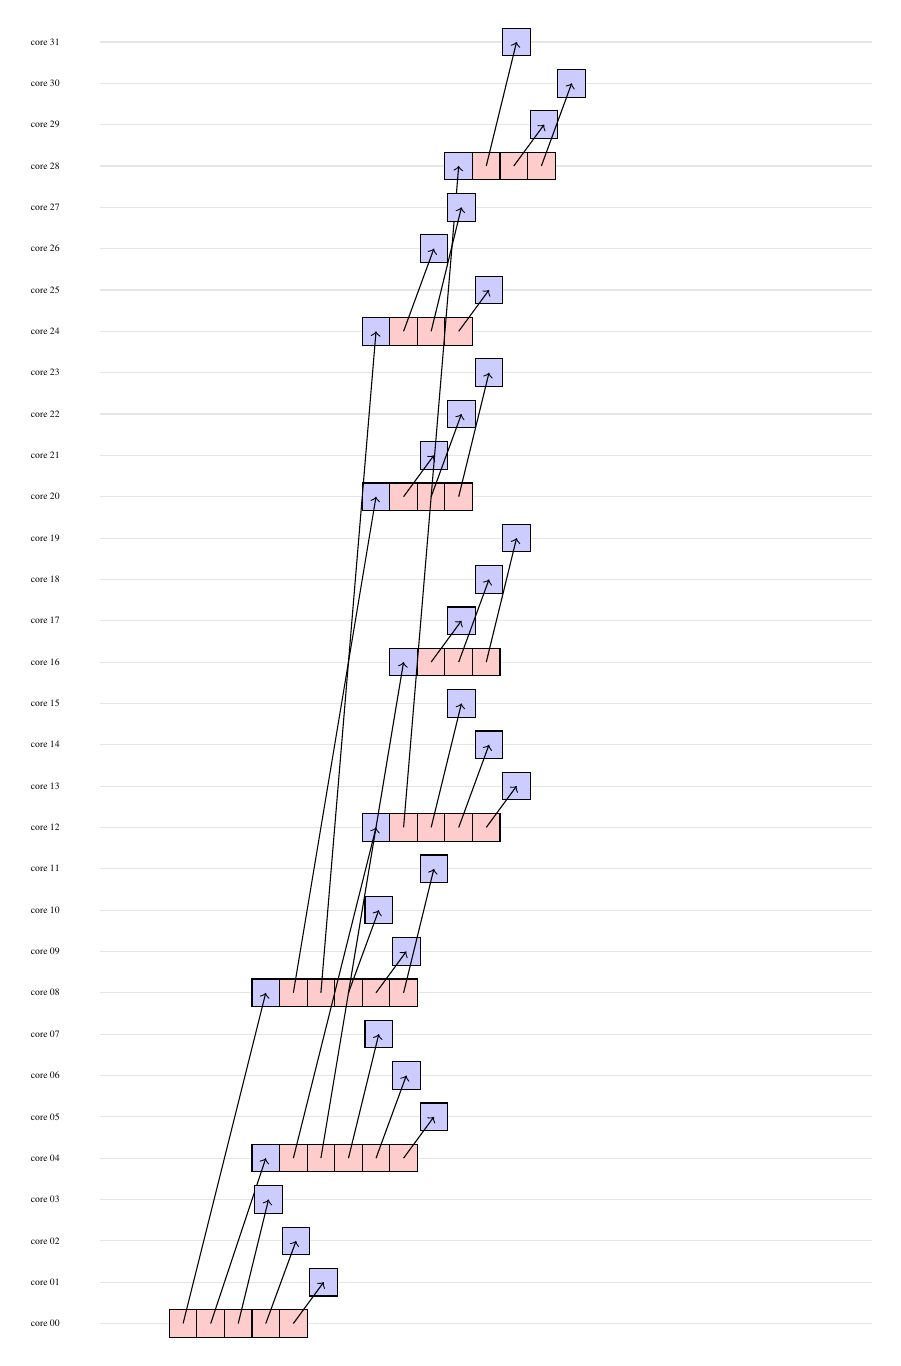
\begin{tikzpicture}[scale=.35,transform shape]
    % Insert visualization
    \node at (0mm,0mm) {core 00};
\draw[color=black!10] (20mm,0mm) -- (30cm,0mm);
\node at (0mm,15mm) {core 01};
\draw[color=black!10] (20mm,15mm) -- (30cm,15mm);
\node at (0mm,30mm) {core 02};
\draw[color=black!10] (20mm,30mm) -- (30cm,30mm);
\node at (0mm,45mm) {core 03};
\draw[color=black!10] (20mm,45mm) -- (30cm,45mm);
\node at (0mm,60mm) {core 04};
\draw[color=black!10] (20mm,60mm) -- (30cm,60mm);
\node at (0mm,75mm) {core 05};
\draw[color=black!10] (20mm,75mm) -- (30cm,75mm);
\node at (0mm,90mm) {core 06};
\draw[color=black!10] (20mm,90mm) -- (30cm,90mm);
\node at (0mm,105mm) {core 07};
\draw[color=black!10] (20mm,105mm) -- (30cm,105mm);
\node at (0mm,120mm) {core 08};
\draw[color=black!10] (20mm,120mm) -- (30cm,120mm);
\node at (0mm,135mm) {core 09};
\draw[color=black!10] (20mm,135mm) -- (30cm,135mm);
\node at (0mm,150mm) {core 10};
\draw[color=black!10] (20mm,150mm) -- (30cm,150mm);
\node at (0mm,165mm) {core 11};
\draw[color=black!10] (20mm,165mm) -- (30cm,165mm);
\node at (0mm,180mm) {core 12};
\draw[color=black!10] (20mm,180mm) -- (30cm,180mm);
\node at (0mm,195mm) {core 13};
\draw[color=black!10] (20mm,195mm) -- (30cm,195mm);
\node at (0mm,210mm) {core 14};
\draw[color=black!10] (20mm,210mm) -- (30cm,210mm);
\node at (0mm,225mm) {core 15};
\draw[color=black!10] (20mm,225mm) -- (30cm,225mm);
\node at (0mm,240mm) {core 16};
\draw[color=black!10] (20mm,240mm) -- (30cm,240mm);
\node at (0mm,255mm) {core 17};
\draw[color=black!10] (20mm,255mm) -- (30cm,255mm);
\node at (0mm,270mm) {core 18};
\draw[color=black!10] (20mm,270mm) -- (30cm,270mm);
\node at (0mm,285mm) {core 19};
\draw[color=black!10] (20mm,285mm) -- (30cm,285mm);
\node at (0mm,300mm) {core 20};
\draw[color=black!10] (20mm,300mm) -- (30cm,300mm);
\node at (0mm,315mm) {core 21};
\draw[color=black!10] (20mm,315mm) -- (30cm,315mm);
\node at (0mm,330mm) {core 22};
\draw[color=black!10] (20mm,330mm) -- (30cm,330mm);
\node at (0mm,345mm) {core 23};
\draw[color=black!10] (20mm,345mm) -- (30cm,345mm);
\node at (0mm,360mm) {core 24};
\draw[color=black!10] (20mm,360mm) -- (30cm,360mm);
\node at (0mm,375mm) {core 25};
\draw[color=black!10] (20mm,375mm) -- (30cm,375mm);
\node at (0mm,390mm) {core 26};
\draw[color=black!10] (20mm,390mm) -- (30cm,390mm);
\node at (0mm,405mm) {core 27};
\draw[color=black!10] (20mm,405mm) -- (30cm,405mm);
\node at (0mm,420mm) {core 28};
\draw[color=black!10] (20mm,420mm) -- (30cm,420mm);
\node at (0mm,435mm) {core 29};
\draw[color=black!10] (20mm,435mm) -- (30cm,435mm);
\node at (0mm,450mm) {core 30};
\draw[color=black!10] (20mm,450mm) -- (30cm,450mm);
\node at (0mm,465mm) {core 31};
\draw[color=black!10] (20mm,465mm) -- (30cm,465mm);
\node[draw,fill=red!20,minimum size=10mm] (s_0_8) at (50mm,0mm) {};
\node[draw,fill=red!20,minimum size=10mm] (s_0_4) at (60mm,0mm) {};
\node[draw,fill=red!20,minimum size=10mm] (s_0_3) at (70mm,0mm) {};
\node[draw,fill=red!20,minimum size=10mm] (s_0_2) at (80mm,0mm) {};
\node[draw,fill=red!20,minimum size=10mm] (s_0_1) at (90mm,0mm) {};
\node[draw,fill=blue!20,minimum size=10mm] (r_0_8) at (80mm,120mm) {};
\draw[->] (s_0_8.center) -- (r_0_8.center); 
\node[draw,fill=red!20,minimum size=10mm] (s_8_20) at (90mm,120mm) {};
\node[draw,fill=red!20,minimum size=10mm] (s_8_24) at (100mm,120mm) {};
\node[draw,fill=red!20,minimum size=10mm] (s_8_10) at (110mm,120mm) {};
\node[draw,fill=red!20,minimum size=10mm] (s_8_9) at (120mm,120mm) {};
\node[draw,fill=red!20,minimum size=10mm] (s_8_11) at (130mm,120mm) {};
\node[draw,fill=blue!20,minimum size=10mm] (r_0_4) at (80mm,60mm) {};
\draw[->] (s_0_4.center) -- (r_0_4.center); 
\node[draw,fill=red!20,minimum size=10mm] (s_4_12) at (90mm,60mm) {};
\node[draw,fill=red!20,minimum size=10mm] (s_4_16) at (100mm,60mm) {};
\node[draw,fill=red!20,minimum size=10mm] (s_4_7) at (110mm,60mm) {};
\node[draw,fill=red!20,minimum size=10mm] (s_4_6) at (120mm,60mm) {};
\node[draw,fill=red!20,minimum size=10mm] (s_4_5) at (130mm,60mm) {};
\node[draw,fill=blue!20,minimum size=10mm] (r_0_3) at (81mm,45mm) {};
\draw[->] (s_0_3.center) -- (r_0_3.center); 
\node[draw,fill=blue!20,minimum size=10mm] (r_0_2) at (91mm,30mm) {};
\draw[->] (s_0_2.center) -- (r_0_2.center); 
\node[draw,fill=blue!20,minimum size=10mm] (r_0_1) at (101mm,15mm) {};
\draw[->] (s_0_1.center) -- (r_0_1.center); 
\node[draw,fill=blue!20,minimum size=10mm] (r_8_20) at (120mm,300mm) {};
\draw[->] (s_8_20.center) -- (r_8_20.center); 
\node[draw,fill=red!20,minimum size=10mm] (s_20_21) at (130mm,300mm) {};
\node[draw,fill=red!20,minimum size=10mm] (s_20_22) at (140mm,300mm) {};
\node[draw,fill=red!20,minimum size=10mm] (s_20_23) at (150mm,300mm) {};
\node[draw,fill=blue!20,minimum size=10mm] (r_8_24) at (120mm,360mm) {};
\draw[->] (s_8_24.center) -- (r_8_24.center); 
\node[draw,fill=red!20,minimum size=10mm] (s_24_26) at (130mm,360mm) {};
\node[draw,fill=red!20,minimum size=10mm] (s_24_27) at (140mm,360mm) {};
\node[draw,fill=red!20,minimum size=10mm] (s_24_25) at (150mm,360mm) {};
\node[draw,fill=blue!20,minimum size=10mm] (r_4_12) at (120mm,180mm) {};
\draw[->] (s_4_12.center) -- (r_4_12.center); 
\node[draw,fill=red!20,minimum size=10mm] (s_12_28) at (130mm,180mm) {};
\node[draw,fill=red!20,minimum size=10mm] (s_12_15) at (140mm,180mm) {};
\node[draw,fill=red!20,minimum size=10mm] (s_12_14) at (150mm,180mm) {};
\node[draw,fill=red!20,minimum size=10mm] (s_12_13) at (160mm,180mm) {};
\node[draw,fill=blue!20,minimum size=10mm] (r_8_10) at (121mm,150mm) {};
\draw[->] (s_8_10.center) -- (r_8_10.center); 
\node[draw,fill=blue!20,minimum size=10mm] (r_4_7) at (121mm,105mm) {};
\draw[->] (s_4_7.center) -- (r_4_7.center); 
\node[draw,fill=blue!20,minimum size=10mm] (r_4_16) at (130mm,240mm) {};
\draw[->] (s_4_16.center) -- (r_4_16.center); 
\node[draw,fill=red!20,minimum size=10mm] (s_16_17) at (140mm,240mm) {};
\node[draw,fill=red!20,minimum size=10mm] (s_16_18) at (150mm,240mm) {};
\node[draw,fill=red!20,minimum size=10mm] (s_16_19) at (160mm,240mm) {};
\node[draw,fill=blue!20,minimum size=10mm] (r_8_9) at (131mm,135mm) {};
\draw[->] (s_8_9.center) -- (r_8_9.center); 
\node[draw,fill=blue!20,minimum size=10mm] (r_4_6) at (131mm,90mm) {};
\draw[->] (s_4_6.center) -- (r_4_6.center); 
\node[draw,fill=blue!20,minimum size=10mm] (r_4_5) at (141mm,75mm) {};
\draw[->] (s_4_5.center) -- (r_4_5.center); 
\node[draw,fill=blue!20,minimum size=10mm] (r_8_11) at (141mm,165mm) {};
\draw[->] (s_8_11.center) -- (r_8_11.center); 
\node[draw,fill=blue!20,minimum size=10mm] (r_24_26) at (141mm,390mm) {};
\draw[->] (s_24_26.center) -- (r_24_26.center); 
\node[draw,fill=blue!20,minimum size=10mm] (r_20_21) at (141mm,315mm) {};
\draw[->] (s_20_21.center) -- (r_20_21.center); 
\node[draw,fill=blue!20,minimum size=10mm] (r_12_28) at (150mm,420mm) {};
\draw[->] (s_12_28.center) -- (r_12_28.center); 
\node[draw,fill=red!20,minimum size=10mm] (s_28_31) at (160mm,420mm) {};
\node[draw,fill=red!20,minimum size=10mm] (s_28_29) at (170mm,420mm) {};
\node[draw,fill=red!20,minimum size=10mm] (s_28_30) at (180mm,420mm) {};
\node[draw,fill=blue!20,minimum size=10mm] (r_16_17) at (151mm,255mm) {};
\draw[->] (s_16_17.center) -- (r_16_17.center); 
\node[draw,fill=blue!20,minimum size=10mm] (r_20_22) at (151mm,330mm) {};
\draw[->] (s_20_22.center) -- (r_20_22.center); 
\node[draw,fill=blue!20,minimum size=10mm] (r_24_27) at (151mm,405mm) {};
\draw[->] (s_24_27.center) -- (r_24_27.center); 
\node[draw,fill=blue!20,minimum size=10mm] (r_12_15) at (151mm,225mm) {};
\draw[->] (s_12_15.center) -- (r_12_15.center); 
\node[draw,fill=blue!20,minimum size=10mm] (r_20_23) at (161mm,345mm) {};
\draw[->] (s_20_23.center) -- (r_20_23.center); 
\node[draw,fill=blue!20,minimum size=10mm] (r_24_25) at (161mm,375mm) {};
\draw[->] (s_24_25.center) -- (r_24_25.center); 
\node[draw,fill=blue!20,minimum size=10mm] (r_12_14) at (161mm,210mm) {};
\draw[->] (s_12_14.center) -- (r_12_14.center); 
\node[draw,fill=blue!20,minimum size=10mm] (r_16_18) at (161mm,270mm) {};
\draw[->] (s_16_18.center) -- (r_16_18.center); 
\node[draw,fill=blue!20,minimum size=10mm] (r_16_19) at (171mm,285mm) {};
\draw[->] (s_16_19.center) -- (r_16_19.center); 
\node[draw,fill=blue!20,minimum size=10mm] (r_28_31) at (171mm,465mm) {};
\draw[->] (s_28_31.center) -- (r_28_31.center); 
\node[draw,fill=blue!20,minimum size=10mm] (r_12_13) at (171mm,195mm) {};
\draw[->] (s_12_13.center) -- (r_12_13.center); 
\node[draw,fill=blue!20,minimum size=10mm] (r_28_29) at (181mm,435mm) {};
\draw[->] (s_28_29.center) -- (r_28_29.center); 
\node[draw,fill=blue!20,minimum size=10mm] (r_28_30) at (191mm,450mm) {};
\draw[->] (s_28_30.center) -- (r_28_30.center); 

  \end{tikzpicture}
  \caption{Visualization of hierarchical tree broadcast. A binary tree
    spans across NUMA nodes followed by sequential send operations
    within the NUMA node. %
    Red boxes represent send operations, blue boxes represent receive
    operations and arrows messages sent between cores.  }
  \label{fig:visu_hierarchy}
\end{figure}

\begin{figure}[htb]
  \centering
  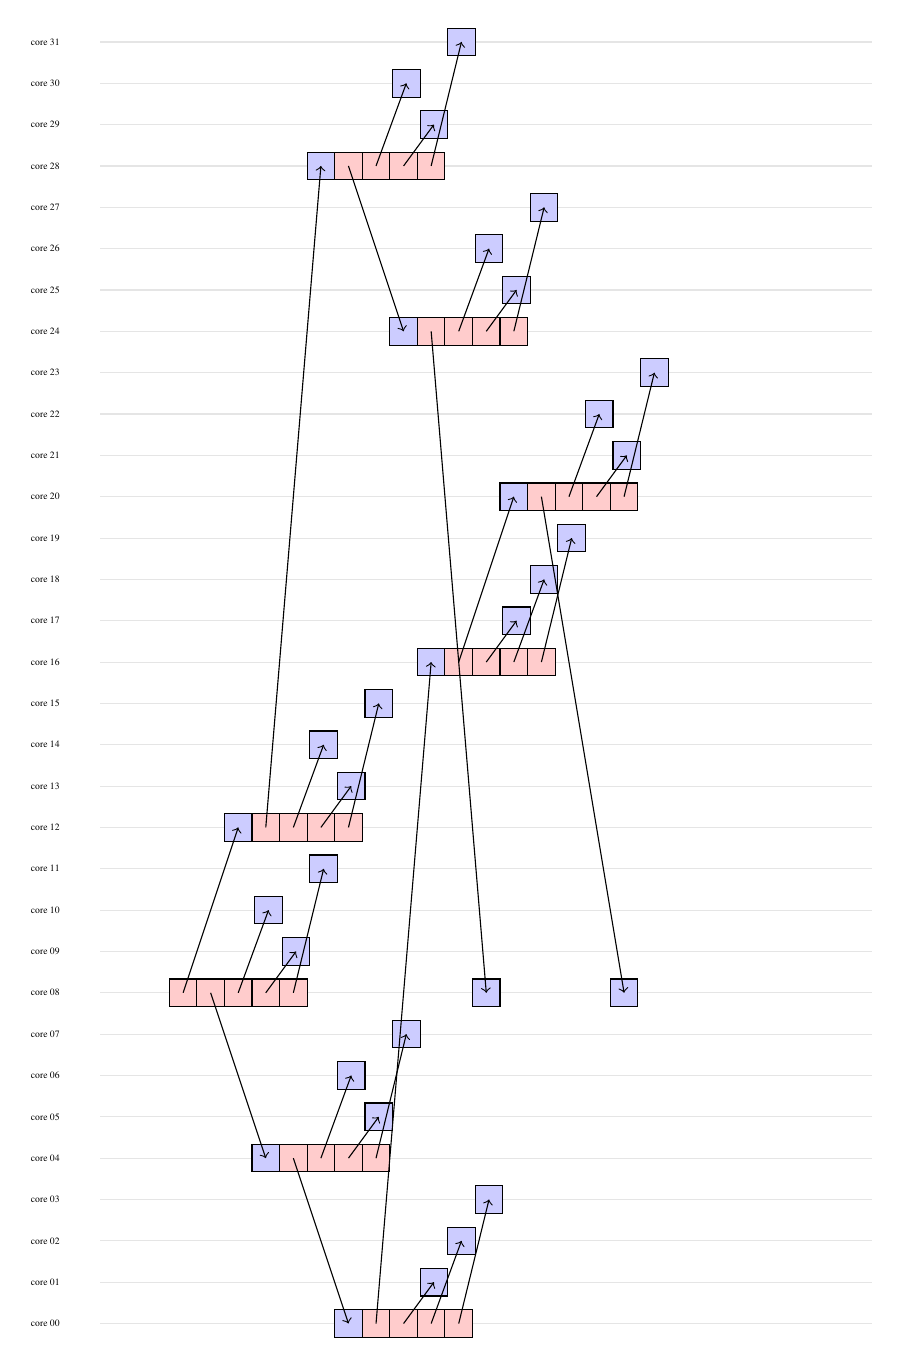
\begin{tikzpicture}[scale=.35,transform shape]
    % Insert visualization
    \node at (0mm,0mm) {core 00};
\draw[color=black!10] (20mm,0mm) -- (30cm,0mm);
\node at (0mm,15mm) {core 01};
\draw[color=black!10] (20mm,15mm) -- (30cm,15mm);
\node at (0mm,30mm) {core 02};
\draw[color=black!10] (20mm,30mm) -- (30cm,30mm);
\node at (0mm,45mm) {core 03};
\draw[color=black!10] (20mm,45mm) -- (30cm,45mm);
\node at (0mm,60mm) {core 04};
\draw[color=black!10] (20mm,60mm) -- (30cm,60mm);
\node at (0mm,75mm) {core 05};
\draw[color=black!10] (20mm,75mm) -- (30cm,75mm);
\node at (0mm,90mm) {core 06};
\draw[color=black!10] (20mm,90mm) -- (30cm,90mm);
\node at (0mm,105mm) {core 07};
\draw[color=black!10] (20mm,105mm) -- (30cm,105mm);
\node at (0mm,120mm) {core 08};
\draw[color=black!10] (20mm,120mm) -- (30cm,120mm);
\node at (0mm,135mm) {core 09};
\draw[color=black!10] (20mm,135mm) -- (30cm,135mm);
\node at (0mm,150mm) {core 10};
\draw[color=black!10] (20mm,150mm) -- (30cm,150mm);
\node at (0mm,165mm) {core 11};
\draw[color=black!10] (20mm,165mm) -- (30cm,165mm);
\node at (0mm,180mm) {core 12};
\draw[color=black!10] (20mm,180mm) -- (30cm,180mm);
\node at (0mm,195mm) {core 13};
\draw[color=black!10] (20mm,195mm) -- (30cm,195mm);
\node at (0mm,210mm) {core 14};
\draw[color=black!10] (20mm,210mm) -- (30cm,210mm);
\node at (0mm,225mm) {core 15};
\draw[color=black!10] (20mm,225mm) -- (30cm,225mm);
\node at (0mm,240mm) {core 16};
\draw[color=black!10] (20mm,240mm) -- (30cm,240mm);
\node at (0mm,255mm) {core 17};
\draw[color=black!10] (20mm,255mm) -- (30cm,255mm);
\node at (0mm,270mm) {core 18};
\draw[color=black!10] (20mm,270mm) -- (30cm,270mm);
\node at (0mm,285mm) {core 19};
\draw[color=black!10] (20mm,285mm) -- (30cm,285mm);
\node at (0mm,300mm) {core 20};
\draw[color=black!10] (20mm,300mm) -- (30cm,300mm);
\node at (0mm,315mm) {core 21};
\draw[color=black!10] (20mm,315mm) -- (30cm,315mm);
\node at (0mm,330mm) {core 22};
\draw[color=black!10] (20mm,330mm) -- (30cm,330mm);
\node at (0mm,345mm) {core 23};
\draw[color=black!10] (20mm,345mm) -- (30cm,345mm);
\node at (0mm,360mm) {core 24};
\draw[color=black!10] (20mm,360mm) -- (30cm,360mm);
\node at (0mm,375mm) {core 25};
\draw[color=black!10] (20mm,375mm) -- (30cm,375mm);
\node at (0mm,390mm) {core 26};
\draw[color=black!10] (20mm,390mm) -- (30cm,390mm);
\node at (0mm,405mm) {core 27};
\draw[color=black!10] (20mm,405mm) -- (30cm,405mm);
\node at (0mm,420mm) {core 28};
\draw[color=black!10] (20mm,420mm) -- (30cm,420mm);
\node at (0mm,435mm) {core 29};
\draw[color=black!10] (20mm,435mm) -- (30cm,435mm);
\node at (0mm,450mm) {core 30};
\draw[color=black!10] (20mm,450mm) -- (30cm,450mm);
\node at (0mm,465mm) {core 31};
\draw[color=black!10] (20mm,465mm) -- (30cm,465mm);
\node[draw,fill=red!20,minimum size=10mm] (s_8_12) at (50mm,120mm) {};
\node[draw,fill=red!20,minimum size=10mm] (s_8_4) at (60mm,120mm) {};
\node[draw,fill=red!20,minimum size=10mm] (s_8_10) at (70mm,120mm) {};
\node[draw,fill=red!20,minimum size=10mm] (s_8_9) at (80mm,120mm) {};
\node[draw,fill=red!20,minimum size=10mm] (s_8_11) at (90mm,120mm) {};
\node[draw,fill=blue!20,minimum size=10mm] (r_8_12) at (70mm,180mm) {};
\draw[->] (s_8_12.center) -- (r_8_12.center); 
\node[draw,fill=red!20,minimum size=10mm] (s_12_28) at (80mm,180mm) {};
\node[draw,fill=red!20,minimum size=10mm] (s_12_14) at (90mm,180mm) {};
\node[draw,fill=red!20,minimum size=10mm] (s_12_13) at (100mm,180mm) {};
\node[draw,fill=red!20,minimum size=10mm] (s_12_15) at (110mm,180mm) {};
\node[draw,fill=blue!20,minimum size=10mm] (r_8_4) at (80mm,60mm) {};
\draw[->] (s_8_4.center) -- (r_8_4.center); 
\node[draw,fill=red!20,minimum size=10mm] (s_4_0) at (90mm,60mm) {};
\node[draw,fill=red!20,minimum size=10mm] (s_4_6) at (100mm,60mm) {};
\node[draw,fill=red!20,minimum size=10mm] (s_4_5) at (110mm,60mm) {};
\node[draw,fill=red!20,minimum size=10mm] (s_4_7) at (120mm,60mm) {};
\node[draw,fill=blue!20,minimum size=10mm] (r_8_10) at (81mm,150mm) {};
\draw[->] (s_8_10.center) -- (r_8_10.center); 
\node[draw,fill=blue!20,minimum size=10mm] (r_8_9) at (91mm,135mm) {};
\draw[->] (s_8_9.center) -- (r_8_9.center); 
\node[draw,fill=blue!20,minimum size=10mm] (r_12_28) at (100mm,420mm) {};
\draw[->] (s_12_28.center) -- (r_12_28.center); 
\node[draw,fill=red!20,minimum size=10mm] (s_28_24) at (110mm,420mm) {};
\node[draw,fill=red!20,minimum size=10mm] (s_28_30) at (120mm,420mm) {};
\node[draw,fill=red!20,minimum size=10mm] (s_28_29) at (130mm,420mm) {};
\node[draw,fill=red!20,minimum size=10mm] (s_28_31) at (140mm,420mm) {};
\node[draw,fill=blue!20,minimum size=10mm] (r_8_11) at (101mm,165mm) {};
\draw[->] (s_8_11.center) -- (r_8_11.center); 
\node[draw,fill=blue!20,minimum size=10mm] (r_12_14) at (101mm,210mm) {};
\draw[->] (s_12_14.center) -- (r_12_14.center); 
\node[draw,fill=blue!20,minimum size=10mm] (r_4_0) at (110mm,0mm) {};
\draw[->] (s_4_0.center) -- (r_4_0.center); 
\node[draw,fill=red!20,minimum size=10mm] (s_0_16) at (120mm,0mm) {};
\node[draw,fill=red!20,minimum size=10mm] (s_0_1) at (130mm,0mm) {};
\node[draw,fill=red!20,minimum size=10mm] (s_0_2) at (140mm,0mm) {};
\node[draw,fill=red!20,minimum size=10mm] (s_0_3) at (150mm,0mm) {};
\node[draw,fill=blue!20,minimum size=10mm] (r_4_6) at (111mm,90mm) {};
\draw[->] (s_4_6.center) -- (r_4_6.center); 
\node[draw,fill=blue!20,minimum size=10mm] (r_12_13) at (111mm,195mm) {};
\draw[->] (s_12_13.center) -- (r_12_13.center); 
\node[draw,fill=blue!20,minimum size=10mm] (r_4_5) at (121mm,75mm) {};
\draw[->] (s_4_5.center) -- (r_4_5.center); 
\node[draw,fill=blue!20,minimum size=10mm] (r_12_15) at (121mm,225mm) {};
\draw[->] (s_12_15.center) -- (r_12_15.center); 
\node[draw,fill=blue!20,minimum size=10mm] (r_28_24) at (130mm,360mm) {};
\draw[->] (s_28_24.center) -- (r_28_24.center); 
\node[draw,fill=red!20,minimum size=10mm] (s_24_8) at (140mm,360mm) {};
\node[draw,fill=red!20,minimum size=10mm] (s_24_26) at (150mm,360mm) {};
\node[draw,fill=red!20,minimum size=10mm] (s_24_25) at (160mm,360mm) {};
\node[draw,fill=red!20,minimum size=10mm] (s_24_27) at (170mm,360mm) {};
\node[draw,fill=blue!20,minimum size=10mm] (r_28_30) at (131mm,450mm) {};
\draw[->] (s_28_30.center) -- (r_28_30.center); 
\node[draw,fill=blue!20,minimum size=10mm] (r_4_7) at (131mm,105mm) {};
\draw[->] (s_4_7.center) -- (r_4_7.center); 
\node[draw,fill=blue!20,minimum size=10mm] (r_0_16) at (140mm,240mm) {};
\draw[->] (s_0_16.center) -- (r_0_16.center); 
\node[draw,fill=red!20,minimum size=10mm] (s_16_20) at (150mm,240mm) {};
\node[draw,fill=red!20,minimum size=10mm] (s_16_17) at (160mm,240mm) {};
\node[draw,fill=red!20,minimum size=10mm] (s_16_18) at (170mm,240mm) {};
\node[draw,fill=red!20,minimum size=10mm] (s_16_19) at (180mm,240mm) {};
\node[draw,fill=blue!20,minimum size=10mm] (r_28_29) at (141mm,435mm) {};
\draw[->] (s_28_29.center) -- (r_28_29.center); 
\node[draw,fill=blue!20,minimum size=10mm] (r_0_1) at (141mm,15mm) {};
\draw[->] (s_0_1.center) -- (r_0_1.center); 
\node[draw,fill=blue!20,minimum size=10mm] (r_0_2) at (151mm,30mm) {};
\draw[->] (s_0_2.center) -- (r_0_2.center); 
\node[draw,fill=blue!20,minimum size=10mm] (r_28_31) at (151mm,465mm) {};
\draw[->] (s_28_31.center) -- (r_28_31.center); 
\node[draw,fill=blue!20,minimum size=10mm] (r_24_8) at (160mm,120mm) {};
\draw[->] (s_24_8.center) -- (r_24_8.center); 
\node[draw,fill=blue!20,minimum size=10mm] (r_0_3) at (161mm,45mm) {};
\draw[->] (s_0_3.center) -- (r_0_3.center); 
\node[draw,fill=blue!20,minimum size=10mm] (r_24_26) at (161mm,390mm) {};
\draw[->] (s_24_26.center) -- (r_24_26.center); 
\node[draw,fill=blue!20,minimum size=10mm] (r_16_20) at (170mm,300mm) {};
\draw[->] (s_16_20.center) -- (r_16_20.center); 
\node[draw,fill=red!20,minimum size=10mm] (s_20_8) at (180mm,300mm) {};
\node[draw,fill=red!20,minimum size=10mm] (s_20_22) at (190mm,300mm) {};
\node[draw,fill=red!20,minimum size=10mm] (s_20_21) at (200mm,300mm) {};
\node[draw,fill=red!20,minimum size=10mm] (s_20_23) at (210mm,300mm) {};
\node[draw,fill=blue!20,minimum size=10mm] (r_24_25) at (171mm,375mm) {};
\draw[->] (s_24_25.center) -- (r_24_25.center); 
\node[draw,fill=blue!20,minimum size=10mm] (r_16_17) at (171mm,255mm) {};
\draw[->] (s_16_17.center) -- (r_16_17.center); 
\node[draw,fill=blue!20,minimum size=10mm] (r_16_18) at (181mm,270mm) {};
\draw[->] (s_16_18.center) -- (r_16_18.center); 
\node[draw,fill=blue!20,minimum size=10mm] (r_24_27) at (181mm,405mm) {};
\draw[->] (s_24_27.center) -- (r_24_27.center); 
\node[draw,fill=blue!20,minimum size=10mm] (r_16_19) at (191mm,285mm) {};
\draw[->] (s_16_19.center) -- (r_16_19.center); 
\node[draw,fill=blue!20,minimum size=10mm] (r_20_22) at (201mm,330mm) {};
\draw[->] (s_20_22.center) -- (r_20_22.center); 
\node[draw,fill=blue!20,minimum size=10mm] (r_20_8) at (210mm,120mm) {};
\draw[->] (s_20_8.center) -- (r_20_8.center); 
\node[draw,fill=blue!20,minimum size=10mm] (r_20_21) at (211mm,315mm) {};
\draw[->] (s_20_21.center) -- (r_20_21.center); 
\node[draw,fill=blue!20,minimum size=10mm] (r_20_23) at (221mm,345mm) {};
\draw[->] (s_20_23.center) -- (r_20_23.center); 

  \end{tikzpicture}
  \caption{Visualization of ring based broadcast. Two rings
    spans across NUMA nodes followed by sequential send operations
    within the NUMA node. %
    Red boxes represent send operations, blue boxes represent receive
    operations and arrows messages sent between
    cores. \stefan{Scheduling is broken. If we want acks, we can only
      forward a message along the ring when all the local nodes
      acknowledge a message}}
  \label{fig:visu_ring}
\end{figure}

%-------------------------------------------------
\subsubsection{Real hardware}

\stefan{Describe benchmark application} 
\begin{itemize}
\item One process on every core
\item Management process on core 2 (i.e.\ not core 0)
\item Uses atomic broadcast as described in Section~\ref{sec:implementation}
\end{itemize}

\paragraph{Binary tree on sbrinz2}

Plot~\ref{pgfplot:201305101058} shows the time in cycles until a
message send from core $n$ is received back via the broadcast tree
show in Figure~\ref{fig:binary_tree_sbrinz2}. We were expecting
increasing cost with the depth of the tree. If a message is sent from
one of the leave nodes, it takes longer to receive this message back
on the tree.

The result is quite unexpected. We would expect nodes far down in the
tree to experience a longer waiting time for receiving own messages
back on the tree (due to more hops). This observation does not seem to
be true. 

Lukas Humbel, who was also working on sbrinz1 was observing that the
Barrelfish core IDs might not properly correspond to physical core
IDs. This could explain the numbers we observe in our measurement.

\begin{figure}[htb]
  \centering
  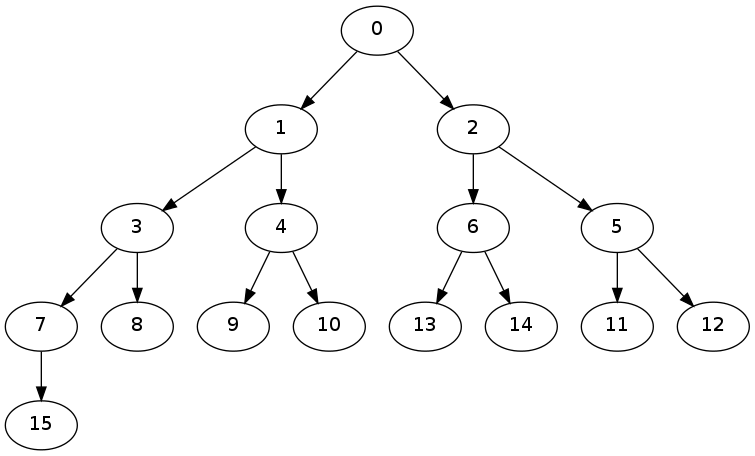
\includegraphics[width=\linewidth]{binary_tree_sbrinz2}
  \caption{Binary tree for sbrinz2}
  \label{fig:binary_tree_sbrinz2}
\end{figure}

\begin{figure}
  \caption{Cost for receiving a message back on the tree. This is the
    time for which the send call needs to be blocked to retain atomic
    broadcast properties.}
  \label{pgfplot:201305101058}
  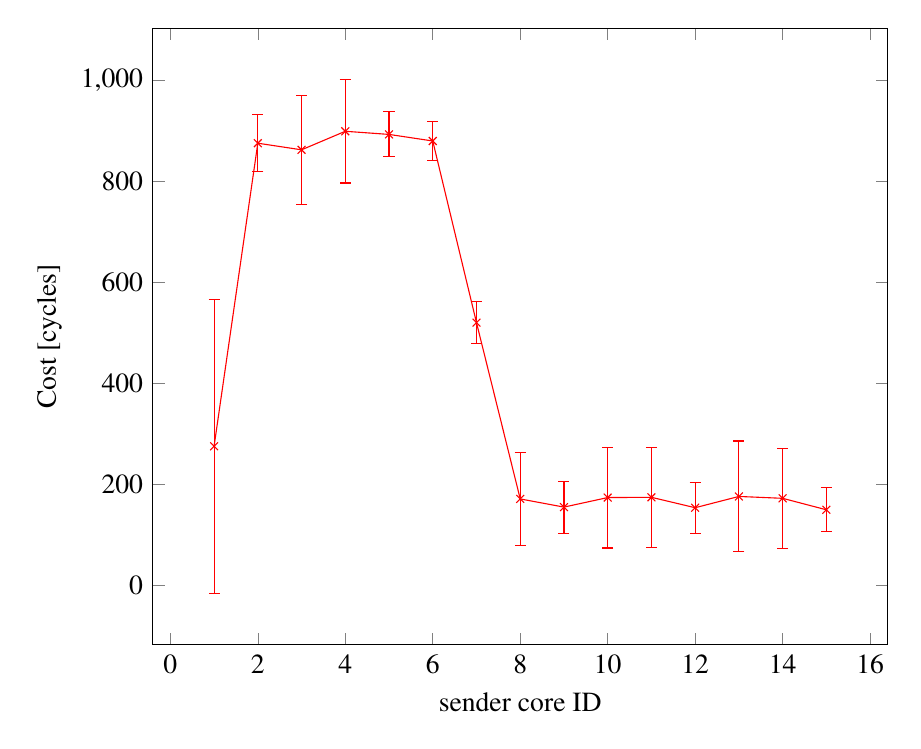
\begin{tikzpicture}
    \begin{axis}[%
        xlabel=sender core ID,%
        ylabel={Cost [cycles]}%
        ]
    \addplot[%
        color=red,%
        mark=x,%  
        error bars/y dir=both,%
        error bars/y explicit%
        ] coordinates {
      (1,276.1) +- (291.3,291.3)
      (2,876.1) +- (56.6,56.6)
      (3,863.0) +- (108.3,108.3)
      (4,899.7) +- (102.3,102.3)
      (5,893.5) +- (44.5,44.5)
      (6,880.5) +- (39.4,39.4)
      (7,520.9) +- (41.7,41.7)
      (8,171.9) +- (91.5,91.5)
      (9,155.7) +- (51.4,51.4)
      (10,174.6) +- (99.9,99.9)
      (11,175.1) +- (99.3,99.3)
      (12,154.5) +- (50.5,50.5)
      (13,176.8) +- (109.7,109.7)
      (14,173.1) +- (99.4,99.4)
      (15,150.4) +- (43.3,43.3)
    };
    \end{axis}
  \end{tikzpicture}
\end{figure}

\paragraph{Older numbers}

Plot~\ref{pgfplot:201303141819} shows the cost of flooding a sub-tree
(with the 50\% worst measurements dropped). The group communication is
based on a binary tree. Core 0 is the root, cores 1 and 2 are its
children etc.

The average cost is really high (probably a scheduling issue). But the
minimal numbers show what is possible. The numbers achieved are easily
explainable. The cost is increasing logarithmic with the number of
nodes reached by the broadcast (as expected). Every level in the tree
adds an additional 2500 to 3000 cycles to the tree. Node 0 takes
significantly longer. I don't know yet why that is.

\begin{figure}
  \caption{Execution time for a broadcast with ACK on gruyere. The
    cost is for execution for the sub-graph starting at the given
    node. Refer to Figure~\ref{fig:qrm_tree_gruyere} for a
    visualization of the broadcast tree used. }
  \label{pgfplot:201303141819}
  \begin{tikzpicture}
    \begin{axis}[
      xlabel=core id,
      scaled y ticks = false, % prevent 10^x stuff
      y tick label style={/pgf/number format/fixed},
      ylabel={cost for subtree [cycles]}]
    \addplot[
      color=red,
      very thin,
      mark=*,
      mark options={%
        scale=.4
      },
      error bars/y dir=both,
      error bars/y explicit] coordinates {
      (0,9932.3) +- (564.4,564.4)
      (1,8240.1) +- (298.5,298.5)
      (2,8259.6) +- (549.4,549.4)
      (3,6206.3) +- (225.1,225.1)
      (4,5914.9) +- (399.2,399.2)
      (5,6033.5) +- (462.2,462.2)
      (6,6070.4) +- (434.3,434.3)
      (7,4530.4) +- (188.6,188.6)
      (8,3163.4) +- (246.1,246.1)
      (9,3403.0) +- (285.3,285.3)
      (10,3650.7) +- (336.5,336.5)
      (11,3559.0) +- (318.8,318.8)
      (12,3558.1) +- (284.8,284.8)
      (13,3567.5) +- (304.5,304.5)
      (14,3476.3) +- (290.2,290.2)
      (15,2711.7) +- (151.9,151.9)
      (16,614.0) +- (17.5,17.5)
      (17,606.2) +- (17.3,17.3)
      (18,636.2) +- (72.5,72.5)
      (19,641.3) +- (46.3,46.3)
      (20,583.8) +- (46.7,46.7)
      (21,577.8) +- (38.3,38.3)
      (22,561.8) +- (18.1,18.1)
      (23,603.5) +- (56.6,56.6)
      (24,589.0) +- (33.4,33.4)
      (25,582.9) +- (33.2,33.2)
      (26,571.7) +- (16.3,16.3)
      (27,581.6) +- (36.6,36.6)
      (28,564.0) +- (16.4,16.4)
      (29,564.0) +- (20.8,20.8)
      (30,551.6) +- (13.0,13.0)
      (31,596.2) +- (51.4,51.4)
    };
    \end{axis}
  \end{tikzpicture}

\end{figure}

%%%%%%%%%%%%%%%%%%%%%%%%%%%%%%%%%%%%%%%%%%%%%%%%%%
%%%%%%%%%%%%%%%%%%%%%%%%%%%%%%%%%%%%%%%%%%%%%%%%%%
\section{Related work}

A multicore aware broadcast has been implemented in~\cite{Tu2008}. It
takes the cache architecture of the machine (and only one particular?)
into consideration for building the broadcast. It is however for
larger messages (starting at 4K) and it does not seem to be performing
very well (numbers are given in microseconds -6). 4K messages are 52
microseconds, which is 150000 cycles. For synchronization primitives,
a cache line is sufficient.

Another tree implementation with MPI in mind was done
in~\cite{Graham2008}. They have comparable numbers to what we found,
but they cannot automatically tune to different machine
characteristics. Our hypothesis is that we can do achieve higher
average performance across a wide range of different multicore
machines without manually adapting the implementation.

Alistarh\etal~\cite{Alistarh2012} show composition of shared-memory
algorithms that perform efficiently under different conditions at
negligible overhead. A similar approach can potentially be applied to
deal with diversity of multicore machines. However, we would have
to extend it to support both shared-memory and message-passing
implementations. 

%%%%%%%%%%%%%%%%%%%%%%%%%%%%%%%%%%%%%%%%%%%%%%%%%%
%%%%%%%%%%%%%%%%%%%%%%%%%%%%%%%%%%%%%%%%%%%%%%%%%%
\section{Future work}

\newcommand{\nary}{$n$-ary\xspace}

\begin{itemize}
\item Keywords: decomposition~\cite{Cavage2013}
\item Other topologies (mainly based on~\cite{Bruck1992}):
  \begin{itemize}
  \item Fibonacci trees: more efficient since nodes further up the
    tree send more messages, but not considering the hierarchy of the
    machine 
  \item \nary trees: play with the out-degree of nodes. The ideal
    value for the out-degree depends on the machine. For
    $t_{propagation} << max(t_{send}, t_{receive})$, $n = 2$ should be
    optimal, since it still increases parallelism, but the latency
    induced by the $n$ send operation is not too high.
  \end{itemize}
\item Think about synchronous implementations and see if they are
  applicable for some of our machines.
\item Arguing that group communication/atomic broadcast is important
  and showing that we can do it well might be enough (appeal to atomic
  broadcasts as the foundation for other distributed algorithms, and
  the MPI primitives, that can/need to be mapped to
  group-communication (have a list of them)
  \begin{itemize}
  \item MPI\_Bcast: send a broadcast message to every node (including
    the sending one)
  \item MPI\_Scatter
  \item MPI\_Gather
  \item MPI\_Reduce
  \end{itemize}
  These primitives are synchronous. They return only once every other
  node received the message. 
\item Need higher-level applications, such as:
  \begin{itemize}
  \item capability system? \stefan{Ask Simon how expensive revocation
      currently is}
  \item a database with replication and consistency maintenance
    \begin{itemize}
    \item SharedDB? (buffers between operators, but no synchronization
      except for access to buffers, which are multiple writers, one
      reader)
    \item Crescando (some kind of state machine replication)
    \end{itemize}
  \end{itemize}
\item MPI collectives (as in~\cite{Tu2008})
\item \emph{Load balancing in a tree} We could build several rings,
  that do not always include all coordinators and work with read- and
  write-sets. We can select these rings such that they nicely
  integrate with the physical topology. They can also have different
  sizes (e.g.\ a smaller one for read operations and larger ones for
  writes).
\item \emph{Aggregation for convergecast} %
  Convergecast is a way of collecting information from nodes (i.e.\ it
  is kind of the reverse of a broadcast). On the return path,
  information can be aggregated. One example is batching, where several
  pieces of information are grouped in the same message to reduce packet
  processing overhead. Another example is aggregation, i.e.\
  pre-processing of data. One example is pre-calculating the average
  value of child messages if the sink node is not interested in
  individual values. %
  Similarly to what has been done in wireless sensor networks (where it
  also matters to reduce the number of messages, but for other reasons:
  power consumption), we can do aggregation in nodes. In difference to
  traditional distributed systems, this works, because it is easy to
  deploy custom software on every node in the network. Classical
  distributed systems do not typically allow this. Furthermore, reducing
  the number of messages at the price of higher complexity does not make
  sense in classical systems. %
  Examples for aggregation: number of nodes agreeing to something, find
  capabilities (concatenate core ids). 
\end{itemize}

%%%%%%%%%%%%%%%%%%%%%%%%%%%%%%%%%%%%%%%%%%%%%%%%%%
\subsection{Octopus}

Octopus is a coordination service implementation for the Barrelfish
Multikernel operating system based on a key-value store
data-backend. It is, however, centralized. The idea is to make Octopus
a decentralized application.

For that, we extend Octopus such that it can be replicated within a
multicore machine. This will retain scalability for future manycore
machines and potentially outperform a centralized version of Octopus
especially in contented systems.

%--------------------------------------------------
\subsubsection{Key-value store}

One foundation block of Octopus is a key-value store. Since there is
only one copy, the data in there is always consistent. If replicated,
some sort of consistency guarantee would have to be implemented. One
example is \emph{linearizability}, i.e.\ ``accesses occur one at a time
in, some sequential order that is consistent with the order of
invocations and responses''~\cite{lynch}.

One concrete idea is to have one copy of the Octopus data-store
replicated on every NUMA node. One core on every node acts as
\emph{coordinator}, we call the other nodes \emph{slaves}.
Coordinators communicate on a ring. Communication on a local NUMA node
can be realized using read-only shared memory for read access. Write
access needs to be globally ordered and hence communication with other
replicas is required. 

Slaves direct their updates to the local coordinator. Coordinators
send the update request $r$ along the ring and wait for them to be
send back. While passing on requests, coordinators can set a flag to
indicate conflicts. A conflict is another colliding request $r_o$ that
is already in flight. I think we will have to send activity vectors
along with this information! Otherwise, the coordinators requesting
$r$ and $r_o$ will both prevent the other thing from happening and
none of them will be applied! Maybe we need a two-phase commit.

The idea of having a ring is somewhat related to SharedDB. It
optimizes for throughput, not latency!

%-------------------------------------------------
\subsubsection{Synchronization}

It is doubtful that a key-value store as a backend for synchronization
primitives as we want to show efficiency rather than ease of use and
flexibility. We probably rather want to implement new synchronization
algorithms from scratch. See Section~\ref{barriers} for ideas.

%%%%%%%%%%%%%%%%%%%%%%%%%%%%%%%%%%%%%%%%%%%%%%%%%%
\subsection{Barriers}
\label{barriers}

The idea is to explore barrier implementations. The idea is to
leverage information about the NUMA topology for better performance of
barrier intensive workloads. Every NUMA node has a coordinator node,
that knows how many threads on that node want to enter the
barrier. There is only local communication (possibly using a
share-memory implementation to exploit the shared cache) until the
point where all NUMA local threads did enter the barrier.  Then there
is ``global'' communication with other coordinators on other nodes
using a message-passing based algorithm. We believe that this scales
better than pure shared-memory implementations due to less
interconnect contention.

We will have to compare the performance of such an implementation with
a purely shared-memory based implementation like pthreads and
something entirely message-passing based like MPI versions.

%%%%%%%%%%%%%%%%%%%%%%%%%%%%%%%%%%%%%%%%%%%%%%%%%%
\newpage
\bibliographystyle{plain}
\bibliography{defs,db,mendeley}

\label{LastPage}

%%%%%%%%%%%%%%%%%%%%%%%%%%%%%%%%%%%%%%%%%%%%%%%%%%

\begin{appendices}

%%%%%%%%%%%%%%%%%%%%%%%%%%%%%%%%%%%%%%%%%%%%%%%%%%
\section{UMP performance}

Figure~\ref{pgfplot:201306061829} shows the breakdown of the cost for
sending UMP messages on ziger1 for communication between core 0 and
all other cores.

Latency is calculated from the round-trip time minus send and receive
time on sender minus processing time on server. However, send time on
one end of a channel seems to overlap with received time on the other
end of the channel, which makes it hard to calculate actual
latency. Thus, we assume the server processing time to be 300 cycles.

\stefan{We can measure latency on a machine with synchronized clocks
  when adding timestamps as payload to the ump messages.}

Send time is independent of which core the message is send
to. Internally, the send operation is a write operation to the local
cache. The cache coherency protocol will then invalidate all other
copies of this line in the system. 

Receive time on the other hand does depend on which cores
communicate. When polling the cache-line, which is invalid at this
time, the cache coherency protocol will transfer this cache-line from
the sending to the receiving core.

\pgfplotsset{width=\linewidth}
\begin{figure}
  \caption{UMP breakdown}
  \label{pgfplot:201306061829}
  \begin{tikzpicture}
    \tikzsetnextfilename{UMP_breakdown_ziger}
    \begin{axis}[
        ybar stacked,ymin=0,legend style={ at={(0.5,-0.20)}, anchor=north, legend columns=-1},
        xlabel={target core},
        ylabel={cycles}
        ]
    \addplot coordinates {
      (1,300.000000)
      (2,300.000000)
      (3,300.000000)
      (4,300.000000)
      (5,300.000000)
      (6,300.000000)
      (7,300.000000)
      (8,300.000000)
      (9,300.000000)
      (10,300.000000)
      (11,300.000000)
      (12,300.000000)
      (13,300.000000)
      (14,300.000000)
      (15,300.000000)
      (16,300.000000)
      (17,300.000000)
      (18,300.000000)
      (19,300.000000)
      (20,300.000000)
      (21,300.000000)
      (22,300.000000)
      (23,300.000000)
    };
    \addplot coordinates {
      (1,244.197531)
      (2,246.407407)
      (3,245.567901)
      (4,244.543210)
      (5,243.530864)
      (6,245.061728)
      (7,245.901235)
      (8,247.481481)
      (9,245.901235)
      (10,243.197531)
      (11,246.530864)
      (12,243.913580)
      (13,246.259259)
      (14,243.469136)
      (15,242.283951)
      (16,244.851852)
      (17,242.209877)
      (18,258.012346)
      (19,256.765432)
      (20,256.592593)
      (21,255.382716)
      (22,258.666667)
      (23,255.567901)
    };
    \addplot coordinates {
      (1,98.388889)
      (2,102.181481)
      (3,101.376543)
      (4,99.783951)
      (5,93.748148)
      (6,187.491358)
      (7,176.212346)
      (8,173.327160)
      (9,178.597531)
      (10,173.375309)
      (11,167.481481)
      (12,175.728395)
      (13,179.177778)
      (14,180.565432)
      (15,183.571605)
      (16,181.665432)
      (17,189.946914)
      (18,331.055556)
      (19,333.632099)
      (20,315.514815)
      (21,313.348148)
      (22,314.414815)
      (23,337.682716)
    };
    \addplot coordinates {
      (1,262.716049)
      (2,250.864198)
      (3,253.271605)
      (4,264.481481)
      (5,262.876543)
      (6,406.592593)
      (7,417.086420)
      (8,414.913580)
      (9,417.024691)
      (10,416.345679)
      (11,417.320988)
      (12,432.172840)
      (13,427.814815)
      (14,429.234568)
      (15,424.814815)
      (16,426.283951)
      (17,425.444444)
      (18,506.333333)
      (19,503.679012)
      (20,518.222222)
      (21,522.506173)
      (22,517.111111)
      (23,504.703704)
    };
     \legend{server cost, send, propagation, receive}
    \end{axis}
  \end{tikzpicture}
\end{figure}


\newpage
\begin{table}[htb]
  \centering
  \begin{tabular}{lrrrrr}
  \toprule
  & \multicolumn{3}{c}{Real hardware [cycles]} & \multicolumn{2}{c}{Simulation [units]} \\
  topology & time & factor & stderr & time & factor \\
  \midrule
  cluster & 3613.32 & 1.024 & 62.39 & 415 & 1.152 \\
  mst & 3527.07 & \colorbox{gray}{1.000} & 64.77 & 384 & 1.067 \\
  bintree & 4013.45 & 1.138 & 84.72 & 450 & 1.250 \\
  sequential & 6956.06 & 1.972 & 494.43 & 1119 & 3.108 \\
  badtree & 4511.57 & 1.279 & 100.63 & 593 & 1.645 \\
  adaptivetree & 3980.55 & 1.129 & 50.79 & 360 & \colorbox{gray}{1.000} \\
  \midrule
  \end{tabular}
  \caption{Topology evaluation for \gruyere}
  \label{tab:gruyere}
\end{table}

\begin{table}[htb]
  \centering
  \begin{tabular}{lrrrrr}
  \toprule
  & \multicolumn{3}{c}{Real hardware} & \multicolumn{2}{c}{Simulation} \\
  topology & time [cycles] & factor & stderr & time [units] & factor \\
  \midrule
  cluster & 3209.08 & 1.042 & 108.07 & 121 & 1.000 \\
  mst & 3080.18 & 1.000 & 63.61 & 232 & 1.917 \\
  bintree & 3337.63 & 1.084 & 81.04 & 343 & 2.835 \\
  sequential & 3874.08 & 1.258 & 303.02 & 454 & 3.752 \\
  badtree & 5673.08 & 1.842 & 65.12 & 565 & 4.669 \\
  \midrule
  \end{tabular}
  \caption{Evaluation of different topologies for ziger1}
  \label{tab:ziger1}
\end{table}

\begin{table}[htb]
  \centering
  \begin{tabular}{lrrrrr}
  \toprule
  & \multicolumn{3}{c}{Real hardware} & \multicolumn{2}{c}{Simulation} \\
  topology & time [cycles] & factor & stderr & time [units] & factor \\
  \midrule
  cluster & 2765.07 & 1.077 & 112.90 & 101 & 1.000 \\
  mst & 2567.22 & 1.000 & 119.15 & 192 & 1.901 \\
  bintree & 2999.23 & 1.168 & 224.12 & 283 & 2.802 \\
  sequential & 3057.91 & 1.191 & 667.68 & 374 & 3.703 \\
  badtree & 4112.49 & 1.602 & 127.63 & 465 & 4.604 \\
  \midrule
  \end{tabular}
  \caption{Evaluation of different topologies for sbrinz1}
  \label{tab:sbrinz1}
\end{table}

\begin{table}[htb]
  \centering
  \begin{tabular}{lrrrrr}
  \toprule
  & \multicolumn{3}{c}{Real hardware} & \multicolumn{2}{c}{Simulation} \\
  topology & time [cycles] & factor & stderr & time [units] & factor \\
  \midrule
  ring & 0.00 & 0.000 & 0.00 & -1 & -1.000 \\
  cluster & 5667.08 & \colorbox{gray}{1.000} & 545.76 & 341 & 1.172 \\
  mst & 5667.08 & \colorbox{gray}{1.000} & 545.76 & 296 & 1.017 \\
  bintree & 6069.18 & 1.071 & 649.31 & 382 & 1.313 \\
  sequential & 8046.20 & 1.420 & 680.75 & 1201 & 4.127 \\
  badtree & 6061.81 & 1.070 & 549.18 & 445 & 1.529 \\
  adaptivetree & 6863.84 & 1.211 & 872.76 & 291 & \colorbox{gray}{1.000} \\
  \midrule
  \end{tabular}
  \caption{Evaluation of different topologies for appenzeller}
  \label{tab:appenzeller}
\end{table}


%\section{Topologies}
\newpage
\subsection{ziger1}
\newpage
\subsubsection{badtree}
\begin{tikzpicture}[]
  % Insert visualization
  \input{graphs/visu_ziger1_badtree}
\end{tikzpicture}
\newpage
\subsubsection{cluster}
\begin{tikzpicture}[]
  % Insert visualization
  \input{graphs/visu_ziger1_cluster}
\end{tikzpicture}
\newpage
\subsubsection{mst}
\begin{tikzpicture}[]
  % Insert visualization
  \input{graphs/visu_ziger1_mst}
\end{tikzpicture}
\newpage
\subsubsection{bintree}
\begin{tikzpicture}[]
  % Insert visualization
  \input{graphs/visu_ziger1_bintree}
\end{tikzpicture}
\newpage
\subsubsection{sequential}
\begin{tikzpicture}[]
  % Insert visualization
  \input{graphs/visu_ziger1_sequential}
\end{tikzpicture}
\newpage
\subsubsection{ring}
\begin{tikzpicture}[]
  % Insert visualization
  \input{graphs/visu_ziger1_ring}
\end{tikzpicture}
\newpage
\subsection{gruyere}
\newpage
\subsubsection{badtree}
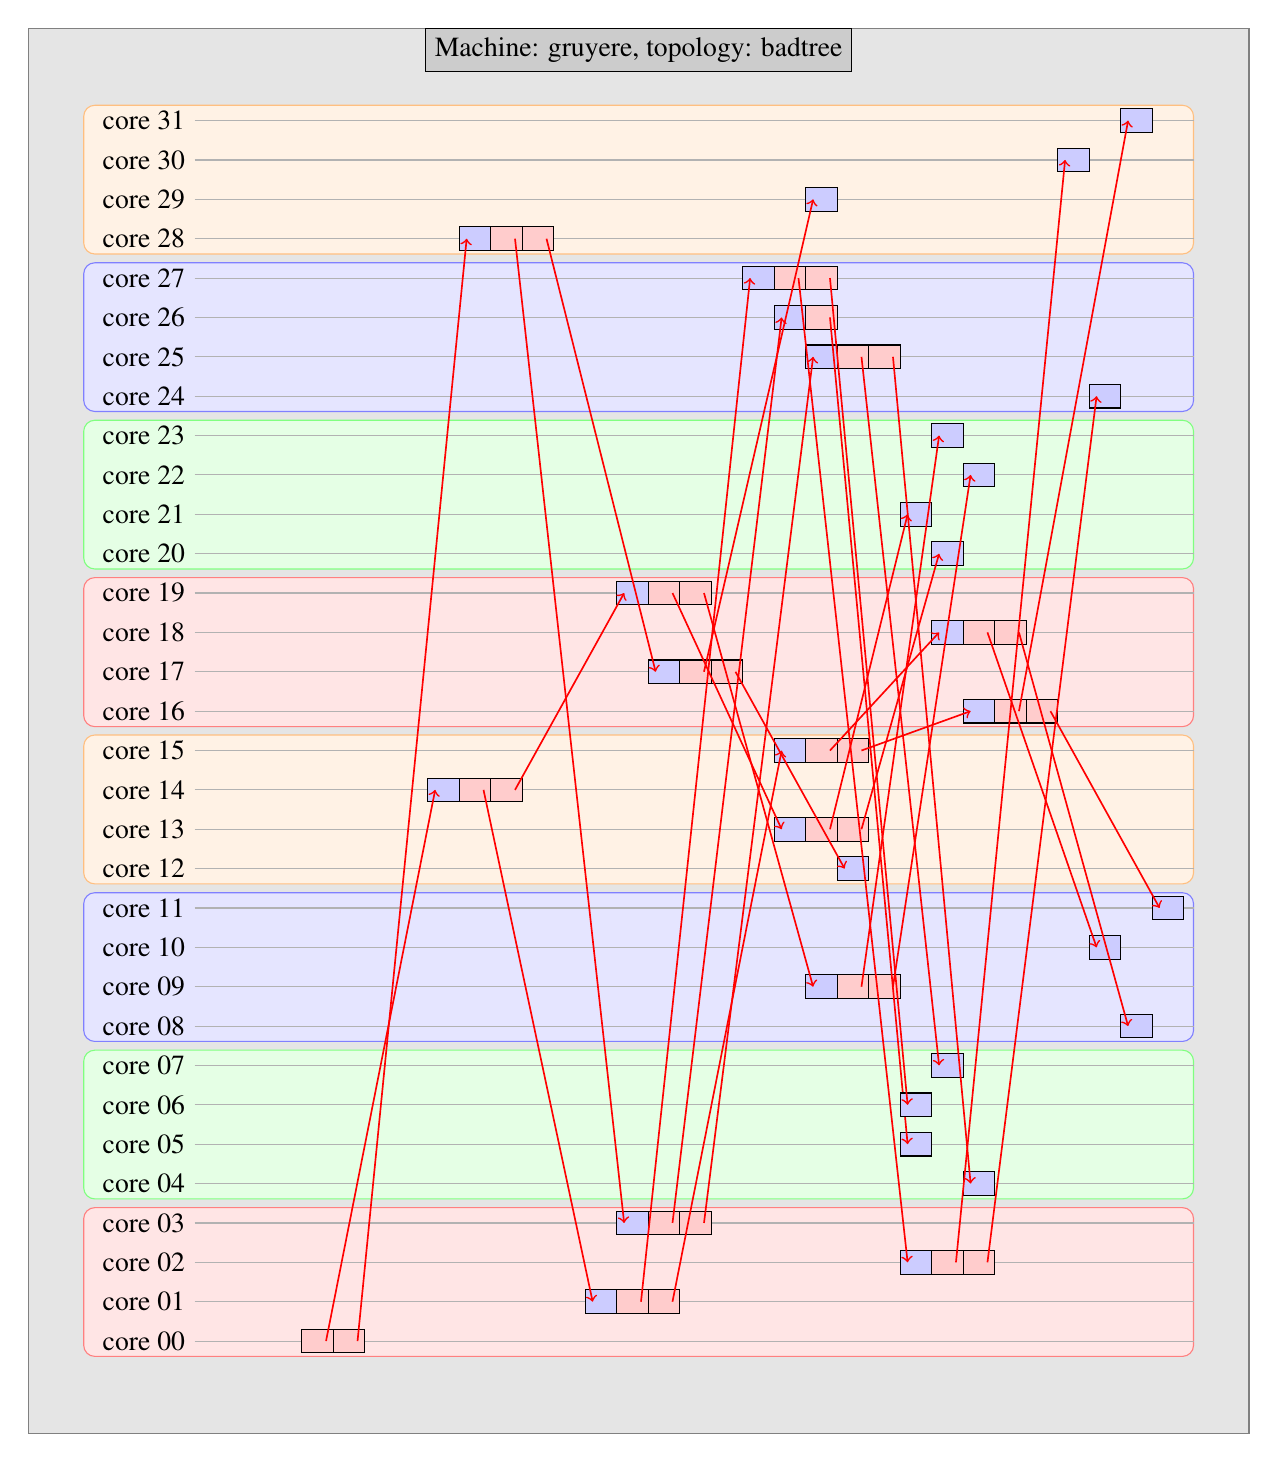
\begin{tikzpicture}[]
  % Insert visualization
  \node (core_0_label) at (0mm,0mm) {core 00};
\node (core_1_label) at (0mm,5mm) {core 01};
\node (core_2_label) at (0mm,10mm) {core 02};
\node (core_3_label) at (0mm,15mm) {core 03};
\node (core_4_label) at (0mm,20mm) {core 04};
\node (core_5_label) at (0mm,25mm) {core 05};
\node (core_6_label) at (0mm,30mm) {core 06};
\node (core_7_label) at (0mm,35mm) {core 07};
\node (core_8_label) at (0mm,40mm) {core 08};
\node (core_9_label) at (0mm,45mm) {core 09};
\node (core_10_label) at (0mm,50mm) {core 10};
\node (core_11_label) at (0mm,55mm) {core 11};
\node (core_12_label) at (0mm,60mm) {core 12};
\node (core_13_label) at (0mm,65mm) {core 13};
\node (core_14_label) at (0mm,70mm) {core 14};
\node (core_15_label) at (0mm,75mm) {core 15};
\node (core_16_label) at (0mm,80mm) {core 16};
\node (core_17_label) at (0mm,85mm) {core 17};
\node (core_18_label) at (0mm,90mm) {core 18};
\node (core_19_label) at (0mm,95mm) {core 19};
\node (core_20_label) at (0mm,100mm) {core 20};
\node (core_21_label) at (0mm,105mm) {core 21};
\node (core_22_label) at (0mm,110mm) {core 22};
\node (core_23_label) at (0mm,115mm) {core 23};
\node (core_24_label) at (0mm,120mm) {core 24};
\node (core_25_label) at (0mm,125mm) {core 25};
\node (core_26_label) at (0mm,130mm) {core 26};
\node (core_27_label) at (0mm,135mm) {core 27};
\node (core_28_label) at (0mm,140mm) {core 28};
\node (core_29_label) at (0mm,145mm) {core 29};
\node (core_30_label) at (0mm,150mm) {core 30};
\node (core_31_label) at (0mm,155mm) {core 31};
\node[draw,fill=red!20,minimum width=4mm, minimum height=3mm,anchor=west] (s_0_14) at (20mm,0mm) {};
\node[draw,fill=red!20,minimum width=4mm, minimum height=3mm,anchor=west] (s_0_28) at (24mm,0mm) {};
\node[draw,fill=blue!20,minimum width=4mm, minimum height=3mm,anchor=west] (r_0_14) at (36mm,70mm) {};
\draw[->,semithick,color=red] ($(s_0_14.east)-(1mm,0mm)$) -- ($(r_0_14.west)+(1mm,0mm)$); 
\node[draw,fill=red!20,minimum width=4mm, minimum height=3mm,anchor=west] (s_14_1) at (40mm,70mm) {};
\node[draw,fill=red!20,minimum width=4mm, minimum height=3mm,anchor=west] (s_14_19) at (44mm,70mm) {};
\node[draw,fill=blue!20,minimum width=4mm, minimum height=3mm,anchor=west] (r_0_28) at (40mm,140mm) {};
\draw[->,semithick,color=red] ($(s_0_28.east)-(1mm,0mm)$) -- ($(r_0_28.west)+(1mm,0mm)$); 
\node[draw,fill=red!20,minimum width=4mm, minimum height=3mm,anchor=west] (s_28_3) at (44mm,140mm) {};
\node[draw,fill=red!20,minimum width=4mm, minimum height=3mm,anchor=west] (s_28_17) at (48mm,140mm) {};
\node[draw,fill=blue!20,minimum width=4mm, minimum height=3mm,anchor=west] (r_14_1) at (56mm,5mm) {};
\draw[->,semithick,color=red] ($(s_14_1.east)-(1mm,0mm)$) -- ($(r_14_1.west)+(1mm,0mm)$); 
\node[draw,fill=red!20,minimum width=4mm, minimum height=3mm,anchor=west] (s_1_27) at (60mm,5mm) {};
\node[draw,fill=red!20,minimum width=4mm, minimum height=3mm,anchor=west] (s_1_15) at (64mm,5mm) {};
\node[draw,fill=blue!20,minimum width=4mm, minimum height=3mm,anchor=west] (r_28_3) at (60mm,15mm) {};
\draw[->,semithick,color=red] ($(s_28_3.east)-(1mm,0mm)$) -- ($(r_28_3.west)+(1mm,0mm)$); 
\node[draw,fill=red!20,minimum width=4mm, minimum height=3mm,anchor=west] (s_3_26) at (64mm,15mm) {};
\node[draw,fill=red!20,minimum width=4mm, minimum height=3mm,anchor=west] (s_3_25) at (68mm,15mm) {};
\node[draw,fill=blue!20,minimum width=4mm, minimum height=3mm,anchor=west] (r_14_19) at (60mm,95mm) {};
\draw[->,semithick,color=red] ($(s_14_19.east)-(1mm,0mm)$) -- ($(r_14_19.west)+(1mm,0mm)$); 
\node[draw,fill=red!20,minimum width=4mm, minimum height=3mm,anchor=west] (s_19_13) at (64mm,95mm) {};
\node[draw,fill=red!20,minimum width=4mm, minimum height=3mm,anchor=west] (s_19_9) at (68mm,95mm) {};
\node[draw,fill=blue!20,minimum width=4mm, minimum height=3mm,anchor=west] (r_28_17) at (64mm,85mm) {};
\draw[->,semithick,color=red] ($(s_28_17.east)-(1mm,0mm)$) -- ($(r_28_17.west)+(1mm,0mm)$); 
\node[draw,fill=red!20,minimum width=4mm, minimum height=3mm,anchor=west] (s_17_29) at (68mm,85mm) {};
\node[draw,fill=red!20,minimum width=4mm, minimum height=3mm,anchor=west] (s_17_12) at (72mm,85mm) {};
\node[draw,fill=blue!20,minimum width=4mm, minimum height=3mm,anchor=west] (r_1_27) at (76mm,135mm) {};
\draw[->,semithick,color=red] ($(s_1_27.east)-(1mm,0mm)$) -- ($(r_1_27.west)+(1mm,0mm)$); 
\node[draw,fill=red!20,minimum width=4mm, minimum height=3mm,anchor=west] (s_27_2) at (80mm,135mm) {};
\node[draw,fill=red!20,minimum width=4mm, minimum height=3mm,anchor=west] (s_27_6) at (84mm,135mm) {};
\node[draw,fill=blue!20,minimum width=4mm, minimum height=3mm,anchor=west] (r_19_13) at (80mm,65mm) {};
\draw[->,semithick,color=red] ($(s_19_13.east)-(1mm,0mm)$) -- ($(r_19_13.west)+(1mm,0mm)$); 
\node[draw,fill=red!20,minimum width=4mm, minimum height=3mm,anchor=west] (s_13_21) at (84mm,65mm) {};
\node[draw,fill=red!20,minimum width=4mm, minimum height=3mm,anchor=west] (s_13_20) at (88mm,65mm) {};
\node[draw,fill=blue!20,minimum width=4mm, minimum height=3mm,anchor=west] (r_1_15) at (80mm,75mm) {};
\draw[->,semithick,color=red] ($(s_1_15.east)-(1mm,0mm)$) -- ($(r_1_15.west)+(1mm,0mm)$); 
\node[draw,fill=red!20,minimum width=4mm, minimum height=3mm,anchor=west] (s_15_18) at (84mm,75mm) {};
\node[draw,fill=red!20,minimum width=4mm, minimum height=3mm,anchor=west] (s_15_16) at (88mm,75mm) {};
\node[draw,fill=blue!20,minimum width=4mm, minimum height=3mm,anchor=west] (r_3_26) at (80mm,130mm) {};
\draw[->,semithick,color=red] ($(s_3_26.east)-(1mm,0mm)$) -- ($(r_3_26.west)+(1mm,0mm)$); 
\node[draw,fill=red!20,minimum width=4mm, minimum height=3mm,anchor=west] (s_26_5) at (84mm,130mm) {};
\node[draw,fill=blue!20,minimum width=4mm, minimum height=3mm,anchor=west] (r_19_9) at (84mm,45mm) {};
\draw[->,semithick,color=red] ($(s_19_9.east)-(1mm,0mm)$) -- ($(r_19_9.west)+(1mm,0mm)$); 
\node[draw,fill=red!20,minimum width=4mm, minimum height=3mm,anchor=west] (s_9_23) at (88mm,45mm) {};
\node[draw,fill=red!20,minimum width=4mm, minimum height=3mm,anchor=west] (s_9_22) at (92mm,45mm) {};
\node[draw,fill=blue!20,minimum width=4mm, minimum height=3mm,anchor=west] (r_17_29) at (84mm,145mm) {};
\draw[->,semithick,color=red] ($(s_17_29.east)-(1mm,0mm)$) -- ($(r_17_29.west)+(1mm,0mm)$); 
\node[draw,fill=blue!20,minimum width=4mm, minimum height=3mm,anchor=west] (r_3_25) at (84mm,125mm) {};
\draw[->,semithick,color=red] ($(s_3_25.east)-(1mm,0mm)$) -- ($(r_3_25.west)+(1mm,0mm)$); 
\node[draw,fill=red!20,minimum width=4mm, minimum height=3mm,anchor=west] (s_25_7) at (88mm,125mm) {};
\node[draw,fill=red!20,minimum width=4mm, minimum height=3mm,anchor=west] (s_25_4) at (92mm,125mm) {};
\node[draw,fill=blue!20,minimum width=4mm, minimum height=3mm,anchor=west] (r_17_12) at (88mm,60mm) {};
\draw[->,semithick,color=red] ($(s_17_12.east)-(1mm,0mm)$) -- ($(r_17_12.west)+(1mm,0mm)$); 
\node[draw,fill=blue!20,minimum width=4mm, minimum height=3mm,anchor=west] (r_26_5) at (96mm,25mm) {};
\draw[->,semithick,color=red] ($(s_26_5.east)-(1mm,0mm)$) -- ($(r_26_5.west)+(1mm,0mm)$); 
\node[draw,fill=blue!20,minimum width=4mm, minimum height=3mm,anchor=west] (r_13_21) at (96mm,105mm) {};
\draw[->,semithick,color=red] ($(s_13_21.east)-(1mm,0mm)$) -- ($(r_13_21.west)+(1mm,0mm)$); 
\node[draw,fill=blue!20,minimum width=4mm, minimum height=3mm,anchor=west] (r_27_6) at (96mm,30mm) {};
\draw[->,semithick,color=red] ($(s_27_6.east)-(1mm,0mm)$) -- ($(r_27_6.west)+(1mm,0mm)$); 
\node[draw,fill=blue!20,minimum width=4mm, minimum height=3mm,anchor=west] (r_27_2) at (96mm,10mm) {};
\draw[->,semithick,color=red] ($(s_27_2.east)-(1mm,0mm)$) -- ($(r_27_2.west)+(1mm,0mm)$); 
\node[draw,fill=red!20,minimum width=4mm, minimum height=3mm,anchor=west] (s_2_30) at (100mm,10mm) {};
\node[draw,fill=red!20,minimum width=4mm, minimum height=3mm,anchor=west] (s_2_24) at (104mm,10mm) {};
\node[draw,fill=blue!20,minimum width=4mm, minimum height=3mm,anchor=west] (r_9_23) at (100mm,115mm) {};
\draw[->,semithick,color=red] ($(s_9_23.east)-(1mm,0mm)$) -- ($(r_9_23.west)+(1mm,0mm)$); 
\node[draw,fill=blue!20,minimum width=4mm, minimum height=3mm,anchor=west] (r_15_18) at (100mm,90mm) {};
\draw[->,semithick,color=red] ($(s_15_18.east)-(1mm,0mm)$) -- ($(r_15_18.west)+(1mm,0mm)$); 
\node[draw,fill=red!20,minimum width=4mm, minimum height=3mm,anchor=west] (s_18_10) at (104mm,90mm) {};
\node[draw,fill=red!20,minimum width=4mm, minimum height=3mm,anchor=west] (s_18_8) at (108mm,90mm) {};
\node[draw,fill=blue!20,minimum width=4mm, minimum height=3mm,anchor=west] (r_13_20) at (100mm,100mm) {};
\draw[->,semithick,color=red] ($(s_13_20.east)-(1mm,0mm)$) -- ($(r_13_20.west)+(1mm,0mm)$); 
\node[draw,fill=blue!20,minimum width=4mm, minimum height=3mm,anchor=west] (r_25_7) at (100mm,35mm) {};
\draw[->,semithick,color=red] ($(s_25_7.east)-(1mm,0mm)$) -- ($(r_25_7.west)+(1mm,0mm)$); 
\node[draw,fill=blue!20,minimum width=4mm, minimum height=3mm,anchor=west] (r_25_4) at (104mm,20mm) {};
\draw[->,semithick,color=red] ($(s_25_4.east)-(1mm,0mm)$) -- ($(r_25_4.west)+(1mm,0mm)$); 
\node[draw,fill=blue!20,minimum width=4mm, minimum height=3mm,anchor=west] (r_9_22) at (104mm,110mm) {};
\draw[->,semithick,color=red] ($(s_9_22.east)-(1mm,0mm)$) -- ($(r_9_22.west)+(1mm,0mm)$); 
\node[draw,fill=blue!20,minimum width=4mm, minimum height=3mm,anchor=west] (r_15_16) at (104mm,80mm) {};
\draw[->,semithick,color=red] ($(s_15_16.east)-(1mm,0mm)$) -- ($(r_15_16.west)+(1mm,0mm)$); 
\node[draw,fill=red!20,minimum width=4mm, minimum height=3mm,anchor=west] (s_16_31) at (108mm,80mm) {};
\node[draw,fill=red!20,minimum width=4mm, minimum height=3mm,anchor=west] (s_16_11) at (112mm,80mm) {};
\node[draw,fill=blue!20,minimum width=4mm, minimum height=3mm,anchor=west] (r_2_30) at (116mm,150mm) {};
\draw[->,semithick,color=red] ($(s_2_30.east)-(1mm,0mm)$) -- ($(r_2_30.west)+(1mm,0mm)$); 
\node[draw,fill=blue!20,minimum width=4mm, minimum height=3mm,anchor=west] (r_2_24) at (120mm,120mm) {};
\draw[->,semithick,color=red] ($(s_2_24.east)-(1mm,0mm)$) -- ($(r_2_24.west)+(1mm,0mm)$); 
\node[draw,fill=blue!20,minimum width=4mm, minimum height=3mm,anchor=west] (r_18_10) at (120mm,50mm) {};
\draw[->,semithick,color=red] ($(s_18_10.east)-(1mm,0mm)$) -- ($(r_18_10.west)+(1mm,0mm)$); 
\node[draw,fill=blue!20,minimum width=4mm, minimum height=3mm,anchor=west] (r_18_8) at (124mm,40mm) {};
\draw[->,semithick,color=red] ($(s_18_8.east)-(1mm,0mm)$) -- ($(r_18_8.west)+(1mm,0mm)$); 
\node[draw,fill=blue!20,minimum width=4mm, minimum height=3mm,anchor=west] (r_16_31) at (124mm,155mm) {};
\draw[->,semithick,color=red] ($(s_16_31.east)-(1mm,0mm)$) -- ($(r_16_31.west)+(1mm,0mm)$); 
\node[draw,fill=blue!20,minimum width=4mm, minimum height=3mm,anchor=west] (r_16_11) at (128mm,55mm) {};
\draw[->,semithick,color=red] ($(s_16_11.east)-(1mm,0mm)$) -- ($(r_16_11.west)+(1mm,0mm)$); 
\begin{pgfonlayer}{background}
\node [fit=(core_0_label) (core_1_label) (core_2_label) (core_3_label) (core_4_label) (core_5_label) (core_6_label) (core_7_label) (core_8_label) (core_9_label) (core_10_label) (core_11_label) (core_12_label) (core_13_label) (core_14_label) (core_15_label) (core_16_label) (core_17_label) (core_18_label) (core_19_label) (core_20_label) (core_21_label) (core_22_label) (core_23_label) (core_24_label) (core_25_label) (core_26_label) (core_27_label) (core_28_label) (core_29_label) (core_30_label) (core_31_label) (s_0_14) (s_0_28) (r_0_14) (s_14_1) (s_14_19) (r_0_28) (s_28_3) (s_28_17) (r_14_1) (s_1_27) (s_1_15) (r_14_19) (s_19_13) (s_19_9) (r_28_3) (s_3_26) (s_3_25) (r_28_17) (s_17_29) (s_17_12) (r_1_27) (s_27_2) (s_27_6) (r_3_26) (s_26_5) (r_1_15) (s_15_18) (s_15_16) (r_19_13) (s_13_21) (s_13_20) (r_3_25) (s_25_7) (s_25_4) (r_17_29) (r_19_9) (s_9_23) (s_9_22) (r_17_12) (r_27_2) (s_2_30) (s_2_24) (r_13_21) (r_27_6) (r_26_5) (r_13_20) (r_25_7) (r_15_18) (s_18_10) (s_18_8) (r_9_23) (r_25_4) (r_15_16) (s_16_31) (s_16_11) (r_9_22) (r_2_30) (r_18_10) (r_2_24) (r_18_8) (r_16_31) (r_16_11) (core_0_label) (core_1_label) (core_2_label) (core_3_label) (core_4_label) (core_5_label) (core_6_label) (core_7_label) (core_8_label) (core_9_label) (core_10_label) (core_11_label) (core_12_label) (core_13_label) (core_14_label) (core_15_label) (core_16_label) (core_17_label) (core_18_label) (core_19_label) (core_20_label) (core_21_label) (core_22_label) (core_23_label) (core_24_label) (core_25_label) (core_26_label) (core_27_label) (core_28_label) (core_29_label) (core_30_label) (core_31_label) (s_0_14) (s_0_28) (r_0_14) (s_14_1) (s_14_19) (r_0_28) (s_28_3) (s_28_17) (r_14_1) (s_1_27) (s_1_15) (r_28_3) (s_3_26) (s_3_25) (r_14_19) (s_19_13) (s_19_9) (r_28_17) (s_17_29) (s_17_12) (r_1_27) (s_27_2) (s_27_6) (r_19_13) (s_13_21) (s_13_20) (r_1_15) (s_15_18) (s_15_16) (r_3_26) (s_26_5) (r_19_9) (s_9_23) (s_9_22) (r_17_29) (r_3_25) (s_25_7) (s_25_4) (r_17_12) (r_26_5) (r_13_21) (r_27_6) (r_27_2) (s_2_30) (s_2_24) (r_9_23) (r_15_18) (s_18_10) (s_18_8) (r_13_20) (r_25_7) (r_25_4) (r_9_22) (r_15_16) (s_16_31) (s_16_11) (r_2_30) (r_2_24) (r_18_10) (r_18_8) (r_16_31) (r_16_11)] (allobjects) {};
\node [draw=black!50,fill=black!10,fit=(core_0_label) (core_1_label) (core_2_label) (core_3_label) (core_4_label) (core_5_label) (core_6_label) (core_7_label) (core_8_label) (core_9_label) (core_10_label) (core_11_label) (core_12_label) (core_13_label) (core_14_label) (core_15_label) (core_16_label) (core_17_label) (core_18_label) (core_19_label) (core_20_label) (core_21_label) (core_22_label) (core_23_label) (core_24_label) (core_25_label) (core_26_label) (core_27_label) (core_28_label) (core_29_label) (core_30_label) (core_31_label) (s_0_14) (s_0_28) (r_0_14) (s_14_1) (s_14_19) (r_0_28) (s_28_3) (s_28_17) (r_14_1) (s_1_27) (s_1_15) (r_14_19) (s_19_13) (s_19_9) (r_28_3) (s_3_26) (s_3_25) (r_28_17) (s_17_29) (s_17_12) (r_1_27) (s_27_2) (s_27_6) (r_3_26) (s_26_5) (r_1_15) (s_15_18) (s_15_16) (r_19_13) (s_13_21) (s_13_20) (r_3_25) (s_25_7) (s_25_4) (r_17_29) (r_19_9) (s_9_23) (s_9_22) (r_17_12) (r_27_2) (s_2_30) (s_2_24) (r_13_21) (r_27_6) (r_26_5) (r_13_20) (r_25_7) (r_15_18) (s_18_10) (s_18_8) (r_9_23) (r_25_4) (r_15_16) (s_16_31) (s_16_11) (r_9_22) (r_2_30) (r_18_10) (r_2_24) (r_18_8) (r_16_31) (r_16_11) (core_0_label) (core_1_label) (core_2_label) (core_3_label) (core_4_label) (core_5_label) (core_6_label) (core_7_label) (core_8_label) (core_9_label) (core_10_label) (core_11_label) (core_12_label) (core_13_label) (core_14_label) (core_15_label) (core_16_label) (core_17_label) (core_18_label) (core_19_label) (core_20_label) (core_21_label) (core_22_label) (core_23_label) (core_24_label) (core_25_label) (core_26_label) (core_27_label) (core_28_label) (core_29_label) (core_30_label) (core_31_label) (s_0_14) (s_0_28) (r_0_14) (s_14_1) (s_14_19) (r_0_28) (s_28_3) (s_28_17) (r_14_1) (s_1_27) (s_1_15) (r_28_3) (s_3_26) (s_3_25) (r_14_19) (s_19_13) (s_19_9) (r_28_17) (s_17_29) (s_17_12) (r_1_27) (s_27_2) (s_27_6) (r_19_13) (s_13_21) (s_13_20) (r_1_15) (s_15_18) (s_15_16) (r_3_26) (s_26_5) (r_19_9) (s_9_23) (s_9_22) (r_17_29) (r_3_25) (s_25_7) (s_25_4) (r_17_12) (r_26_5) (r_13_21) (r_27_6) (r_27_2) (s_2_30) (s_2_24) (r_9_23) (r_15_18) (s_18_10) (s_18_8) (r_13_20) (r_25_7) (r_25_4) (r_9_22) (r_15_16) (s_16_31) (s_16_11) (r_2_30) (r_2_24) (r_18_10) (r_18_8) (r_16_31) (r_16_11),scale=1.1] (bg) {};
\draw let \p1 = (allobjects.east) in node[] (numa_axis_0) at (\x1,0mm) {};
\draw let \p1 = (allobjects.east) in node[] (numa_axis_1) at (\x1,5mm) {};
\draw let \p1 = (allobjects.east) in node[] (numa_axis_2) at (\x1,10mm) {};
\draw let \p1 = (allobjects.east) in node[] (numa_axis_3) at (\x1,15mm) {};
\draw let \p1 = (allobjects.east) in node[] (numa_axis_4) at (\x1,20mm) {};
\draw let \p1 = (allobjects.east) in node[] (numa_axis_5) at (\x1,25mm) {};
\draw let \p1 = (allobjects.east) in node[] (numa_axis_6) at (\x1,30mm) {};
\draw let \p1 = (allobjects.east) in node[] (numa_axis_7) at (\x1,35mm) {};
\draw let \p1 = (allobjects.east) in node[] (numa_axis_8) at (\x1,40mm) {};
\draw let \p1 = (allobjects.east) in node[] (numa_axis_9) at (\x1,45mm) {};
\draw let \p1 = (allobjects.east) in node[] (numa_axis_10) at (\x1,50mm) {};
\draw let \p1 = (allobjects.east) in node[] (numa_axis_11) at (\x1,55mm) {};
\draw let \p1 = (allobjects.east) in node[] (numa_axis_12) at (\x1,60mm) {};
\draw let \p1 = (allobjects.east) in node[] (numa_axis_13) at (\x1,65mm) {};
\draw let \p1 = (allobjects.east) in node[] (numa_axis_14) at (\x1,70mm) {};
\draw let \p1 = (allobjects.east) in node[] (numa_axis_15) at (\x1,75mm) {};
\draw let \p1 = (allobjects.east) in node[] (numa_axis_16) at (\x1,80mm) {};
\draw let \p1 = (allobjects.east) in node[] (numa_axis_17) at (\x1,85mm) {};
\draw let \p1 = (allobjects.east) in node[] (numa_axis_18) at (\x1,90mm) {};
\draw let \p1 = (allobjects.east) in node[] (numa_axis_19) at (\x1,95mm) {};
\draw let \p1 = (allobjects.east) in node[] (numa_axis_20) at (\x1,100mm) {};
\draw let \p1 = (allobjects.east) in node[] (numa_axis_21) at (\x1,105mm) {};
\draw let \p1 = (allobjects.east) in node[] (numa_axis_22) at (\x1,110mm) {};
\draw let \p1 = (allobjects.east) in node[] (numa_axis_23) at (\x1,115mm) {};
\draw let \p1 = (allobjects.east) in node[] (numa_axis_24) at (\x1,120mm) {};
\draw let \p1 = (allobjects.east) in node[] (numa_axis_25) at (\x1,125mm) {};
\draw let \p1 = (allobjects.east) in node[] (numa_axis_26) at (\x1,130mm) {};
\draw let \p1 = (allobjects.east) in node[] (numa_axis_27) at (\x1,135mm) {};
\draw let \p1 = (allobjects.east) in node[] (numa_axis_28) at (\x1,140mm) {};
\draw let \p1 = (allobjects.east) in node[] (numa_axis_29) at (\x1,145mm) {};
\draw let \p1 = (allobjects.east) in node[] (numa_axis_30) at (\x1,150mm) {};
\draw let \p1 = (allobjects.east) in node[] (numa_axis_31) at (\x1,155mm) {};
\node [yscale=0.85,draw=red!50,fill=red!10,fit=(core_0_label) (core_1_label) (core_2_label) (core_3_label) (s_0_14) (s_0_28) (r_14_1) (s_1_27) (s_1_15) (r_28_3) (s_3_26) (s_3_25) (r_27_2) (s_2_30) (s_2_24) (numa_axis_0.west) (core_0_label) (core_1_label) (core_2_label) (core_3_label) (s_0_14) (s_0_28) (r_14_1) (s_1_27) (s_1_15) (r_28_3) (s_3_26) (s_3_25) (r_27_2) (s_2_30) (s_2_24) (numa_axis_0.west),rounded corners] {};
\node [yscale=0.85,draw=green!50,fill=green!10,fit=(core_4_label) (core_5_label) (core_6_label) (core_7_label) (r_27_6) (r_26_5) (r_25_7) (r_25_4) (numa_axis_4.west) (core_4_label) (core_5_label) (core_6_label) (core_7_label) (r_26_5) (r_27_6) (r_25_7) (r_25_4) (numa_axis_4.west),rounded corners] {};
\node [yscale=0.85,draw=blue!50,fill=blue!10,fit=(core_8_label) (core_9_label) (core_10_label) (core_11_label) (r_19_9) (s_9_23) (s_9_22) (r_18_10) (r_18_8) (r_16_11) (numa_axis_8.west) (core_8_label) (core_9_label) (core_10_label) (core_11_label) (r_19_9) (s_9_23) (s_9_22) (r_18_10) (r_18_8) (r_16_11) (numa_axis_8.west),rounded corners] {};
\node [yscale=0.85,draw=orange!50,fill=orange!10,fit=(core_12_label) (core_13_label) (core_14_label) (core_15_label) (r_0_14) (s_14_1) (s_14_19) (r_1_15) (s_15_18) (s_15_16) (r_19_13) (s_13_21) (s_13_20) (r_17_12) (numa_axis_12.west) (core_12_label) (core_13_label) (core_14_label) (core_15_label) (r_0_14) (s_14_1) (s_14_19) (r_19_13) (s_13_21) (s_13_20) (r_1_15) (s_15_18) (s_15_16) (r_17_12) (numa_axis_12.west),rounded corners] {};
\node [yscale=0.85,draw=red!50,fill=red!10,fit=(core_16_label) (core_17_label) (core_18_label) (core_19_label) (r_14_19) (s_19_13) (s_19_9) (r_28_17) (s_17_29) (s_17_12) (r_15_18) (s_18_10) (s_18_8) (r_15_16) (s_16_31) (s_16_11) (numa_axis_16.west) (core_16_label) (core_17_label) (core_18_label) (core_19_label) (r_14_19) (s_19_13) (s_19_9) (r_28_17) (s_17_29) (s_17_12) (r_15_18) (s_18_10) (s_18_8) (r_15_16) (s_16_31) (s_16_11) (numa_axis_16.west),rounded corners] {};
\node [yscale=0.85,draw=green!50,fill=green!10,fit=(core_20_label) (core_21_label) (core_22_label) (core_23_label) (r_13_21) (r_13_20) (r_9_23) (r_9_22) (numa_axis_20.west) (core_20_label) (core_21_label) (core_22_label) (core_23_label) (r_13_21) (r_9_23) (r_13_20) (r_9_22) (numa_axis_20.west),rounded corners] {};
\node [yscale=0.85,draw=blue!50,fill=blue!10,fit=(core_24_label) (core_25_label) (core_26_label) (core_27_label) (r_1_27) (s_27_2) (s_27_6) (r_3_26) (s_26_5) (r_3_25) (s_25_7) (s_25_4) (r_2_24) (numa_axis_24.west) (core_24_label) (core_25_label) (core_26_label) (core_27_label) (r_1_27) (s_27_2) (s_27_6) (r_3_26) (s_26_5) (r_3_25) (s_25_7) (s_25_4) (r_2_24) (numa_axis_24.west),rounded corners] {};
\node [yscale=0.85,draw=orange!50,fill=orange!10,fit=(core_28_label) (core_29_label) (core_30_label) (core_31_label) (r_0_28) (s_28_3) (s_28_17) (r_17_29) (r_2_30) (r_16_31) (numa_axis_28.west) (core_28_label) (core_29_label) (core_30_label) (core_31_label) (r_0_28) (s_28_3) (s_28_17) (r_17_29) (r_2_30) (r_16_31) (numa_axis_28.west),rounded corners] {};
\draw[color=black!30] let \p1 = (core_10_label.east), \p2 = (allobjects.east) in (\x1,0mm) -- (\x2,0mm);
\draw[color=black!30] let \p1 = (core_10_label.east), \p2 = (allobjects.east) in (\x1,5mm) -- (\x2,5mm);
\draw[color=black!30] let \p1 = (core_10_label.east), \p2 = (allobjects.east) in (\x1,10mm) -- (\x2,10mm);
\draw[color=black!30] let \p1 = (core_10_label.east), \p2 = (allobjects.east) in (\x1,15mm) -- (\x2,15mm);
\draw[color=black!30] let \p1 = (core_10_label.east), \p2 = (allobjects.east) in (\x1,20mm) -- (\x2,20mm);
\draw[color=black!30] let \p1 = (core_10_label.east), \p2 = (allobjects.east) in (\x1,25mm) -- (\x2,25mm);
\draw[color=black!30] let \p1 = (core_10_label.east), \p2 = (allobjects.east) in (\x1,30mm) -- (\x2,30mm);
\draw[color=black!30] let \p1 = (core_10_label.east), \p2 = (allobjects.east) in (\x1,35mm) -- (\x2,35mm);
\draw[color=black!30] let \p1 = (core_10_label.east), \p2 = (allobjects.east) in (\x1,40mm) -- (\x2,40mm);
\draw[color=black!30] let \p1 = (core_10_label.east), \p2 = (allobjects.east) in (\x1,45mm) -- (\x2,45mm);
\draw[color=black!30] let \p1 = (core_10_label.east), \p2 = (allobjects.east) in (\x1,50mm) -- (\x2,50mm);
\draw[color=black!30] let \p1 = (core_10_label.east), \p2 = (allobjects.east) in (\x1,55mm) -- (\x2,55mm);
\draw[color=black!30] let \p1 = (core_10_label.east), \p2 = (allobjects.east) in (\x1,60mm) -- (\x2,60mm);
\draw[color=black!30] let \p1 = (core_10_label.east), \p2 = (allobjects.east) in (\x1,65mm) -- (\x2,65mm);
\draw[color=black!30] let \p1 = (core_10_label.east), \p2 = (allobjects.east) in (\x1,70mm) -- (\x2,70mm);
\draw[color=black!30] let \p1 = (core_10_label.east), \p2 = (allobjects.east) in (\x1,75mm) -- (\x2,75mm);
\draw[color=black!30] let \p1 = (core_10_label.east), \p2 = (allobjects.east) in (\x1,80mm) -- (\x2,80mm);
\draw[color=black!30] let \p1 = (core_10_label.east), \p2 = (allobjects.east) in (\x1,85mm) -- (\x2,85mm);
\draw[color=black!30] let \p1 = (core_10_label.east), \p2 = (allobjects.east) in (\x1,90mm) -- (\x2,90mm);
\draw[color=black!30] let \p1 = (core_10_label.east), \p2 = (allobjects.east) in (\x1,95mm) -- (\x2,95mm);
\draw[color=black!30] let \p1 = (core_10_label.east), \p2 = (allobjects.east) in (\x1,100mm) -- (\x2,100mm);
\draw[color=black!30] let \p1 = (core_10_label.east), \p2 = (allobjects.east) in (\x1,105mm) -- (\x2,105mm);
\draw[color=black!30] let \p1 = (core_10_label.east), \p2 = (allobjects.east) in (\x1,110mm) -- (\x2,110mm);
\draw[color=black!30] let \p1 = (core_10_label.east), \p2 = (allobjects.east) in (\x1,115mm) -- (\x2,115mm);
\draw[color=black!30] let \p1 = (core_10_label.east), \p2 = (allobjects.east) in (\x1,120mm) -- (\x2,120mm);
\draw[color=black!30] let \p1 = (core_10_label.east), \p2 = (allobjects.east) in (\x1,125mm) -- (\x2,125mm);
\draw[color=black!30] let \p1 = (core_10_label.east), \p2 = (allobjects.east) in (\x1,130mm) -- (\x2,130mm);
\draw[color=black!30] let \p1 = (core_10_label.east), \p2 = (allobjects.east) in (\x1,135mm) -- (\x2,135mm);
\draw[color=black!30] let \p1 = (core_10_label.east), \p2 = (allobjects.east) in (\x1,140mm) -- (\x2,140mm);
\draw[color=black!30] let \p1 = (core_10_label.east), \p2 = (allobjects.east) in (\x1,145mm) -- (\x2,145mm);
\draw[color=black!30] let \p1 = (core_10_label.east), \p2 = (allobjects.east) in (\x1,150mm) -- (\x2,150mm);
\draw[color=black!30] let \p1 = (core_10_label.east), \p2 = (allobjects.east) in (\x1,155mm) -- (\x2,155mm);
\node[draw=black,anchor=north,fill=black!20] at (bg.north) {Machine: gruyere, topology: badtree};
\end{pgfonlayer}

\end{tikzpicture}
\newpage
\subsubsection{cluster}
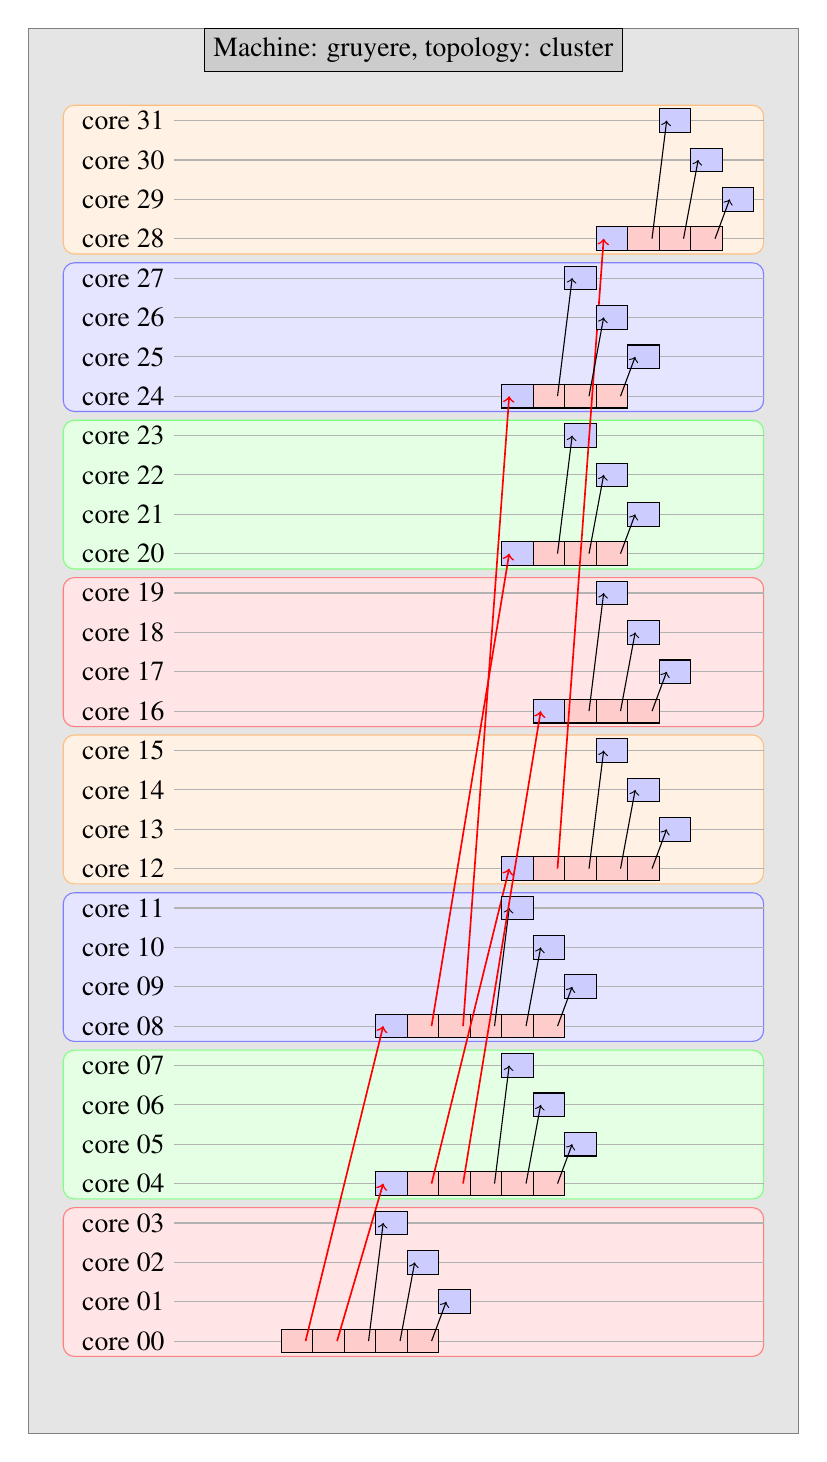
\begin{tikzpicture}[]
  % Insert visualization
  \node (core_0_label) at (0mm,0mm) {core 00};
\node (core_1_label) at (0mm,5mm) {core 01};
\node (core_2_label) at (0mm,10mm) {core 02};
\node (core_3_label) at (0mm,15mm) {core 03};
\node (core_4_label) at (0mm,20mm) {core 04};
\node (core_5_label) at (0mm,25mm) {core 05};
\node (core_6_label) at (0mm,30mm) {core 06};
\node (core_7_label) at (0mm,35mm) {core 07};
\node (core_8_label) at (0mm,40mm) {core 08};
\node (core_9_label) at (0mm,45mm) {core 09};
\node (core_10_label) at (0mm,50mm) {core 10};
\node (core_11_label) at (0mm,55mm) {core 11};
\node (core_12_label) at (0mm,60mm) {core 12};
\node (core_13_label) at (0mm,65mm) {core 13};
\node (core_14_label) at (0mm,70mm) {core 14};
\node (core_15_label) at (0mm,75mm) {core 15};
\node (core_16_label) at (0mm,80mm) {core 16};
\node (core_17_label) at (0mm,85mm) {core 17};
\node (core_18_label) at (0mm,90mm) {core 18};
\node (core_19_label) at (0mm,95mm) {core 19};
\node (core_20_label) at (0mm,100mm) {core 20};
\node (core_21_label) at (0mm,105mm) {core 21};
\node (core_22_label) at (0mm,110mm) {core 22};
\node (core_23_label) at (0mm,115mm) {core 23};
\node (core_24_label) at (0mm,120mm) {core 24};
\node (core_25_label) at (0mm,125mm) {core 25};
\node (core_26_label) at (0mm,130mm) {core 26};
\node (core_27_label) at (0mm,135mm) {core 27};
\node (core_28_label) at (0mm,140mm) {core 28};
\node (core_29_label) at (0mm,145mm) {core 29};
\node (core_30_label) at (0mm,150mm) {core 30};
\node (core_31_label) at (0mm,155mm) {core 31};
\node[draw,fill=red!20,minimum width=4mm, minimum height=3mm,anchor=west] (s_0_8) at (20mm,0mm) {};
\node[draw,fill=red!20,minimum width=4mm, minimum height=3mm,anchor=west] (s_0_4) at (24mm,0mm) {};
\node[draw,fill=red!20,minimum width=4mm, minimum height=3mm,anchor=west] (s_0_3) at (28mm,0mm) {};
\node[draw,fill=red!20,minimum width=4mm, minimum height=3mm,anchor=west] (s_0_2) at (32mm,0mm) {};
\node[draw,fill=red!20,minimum width=4mm, minimum height=3mm,anchor=west] (s_0_1) at (36mm,0mm) {};
\node[draw,fill=blue!20,minimum width=4mm, minimum height=3mm,anchor=west] (r_0_4) at (32mm,20mm) {};
\draw[->,semithick,color=red] ($(s_0_4.east)-(1mm,0mm)$) -- ($(r_0_4.west)+(1mm,0mm)$); 
\node[draw,fill=red!20,minimum width=4mm, minimum height=3mm,anchor=west] (s_4_12) at (36mm,20mm) {};
\node[draw,fill=red!20,minimum width=4mm, minimum height=3mm,anchor=west] (s_4_16) at (40mm,20mm) {};
\node[draw,fill=red!20,minimum width=4mm, minimum height=3mm,anchor=west] (s_4_7) at (44mm,20mm) {};
\node[draw,fill=red!20,minimum width=4mm, minimum height=3mm,anchor=west] (s_4_6) at (48mm,20mm) {};
\node[draw,fill=red!20,minimum width=4mm, minimum height=3mm,anchor=west] (s_4_5) at (52mm,20mm) {};
\node[draw,fill=blue!20,minimum width=4mm, minimum height=3mm,anchor=west] (r_0_8) at (32mm,40mm) {};
\draw[->,semithick,color=red] ($(s_0_8.east)-(1mm,0mm)$) -- ($(r_0_8.west)+(1mm,0mm)$); 
\node[draw,fill=red!20,minimum width=4mm, minimum height=3mm,anchor=west] (s_8_20) at (36mm,40mm) {};
\node[draw,fill=red!20,minimum width=4mm, minimum height=3mm,anchor=west] (s_8_24) at (40mm,40mm) {};
\node[draw,fill=red!20,minimum width=4mm, minimum height=3mm,anchor=west] (s_8_11) at (44mm,40mm) {};
\node[draw,fill=red!20,minimum width=4mm, minimum height=3mm,anchor=west] (s_8_10) at (48mm,40mm) {};
\node[draw,fill=red!20,minimum width=4mm, minimum height=3mm,anchor=west] (s_8_9) at (52mm,40mm) {};
\node[draw,fill=blue!20,minimum width=4mm, minimum height=3mm,anchor=west] (r_0_3) at (32mm,15mm) {};
\draw[->] ($(s_0_3.east)-(1mm,0mm)$) -- ($(r_0_3.west)+(1mm,0mm)$); 
\node[draw,fill=blue!20,minimum width=4mm, minimum height=3mm,anchor=west] (r_0_2) at (36mm,10mm) {};
\draw[->] ($(s_0_2.east)-(1mm,0mm)$) -- ($(r_0_2.west)+(1mm,0mm)$); 
\node[draw,fill=blue!20,minimum width=4mm, minimum height=3mm,anchor=west] (r_0_1) at (40mm,5mm) {};
\draw[->] ($(s_0_1.east)-(1mm,0mm)$) -- ($(r_0_1.west)+(1mm,0mm)$); 
\node[draw,fill=blue!20,minimum width=4mm, minimum height=3mm,anchor=west] (r_8_20) at (48mm,100mm) {};
\draw[->,semithick,color=red] ($(s_8_20.east)-(1mm,0mm)$) -- ($(r_8_20.west)+(1mm,0mm)$); 
\node[draw,fill=red!20,minimum width=4mm, minimum height=3mm,anchor=west] (s_20_23) at (52mm,100mm) {};
\node[draw,fill=red!20,minimum width=4mm, minimum height=3mm,anchor=west] (s_20_22) at (56mm,100mm) {};
\node[draw,fill=red!20,minimum width=4mm, minimum height=3mm,anchor=west] (s_20_21) at (60mm,100mm) {};
\node[draw,fill=blue!20,minimum width=4mm, minimum height=3mm,anchor=west] (r_8_24) at (48mm,120mm) {};
\draw[->,semithick,color=red] ($(s_8_24.east)-(1mm,0mm)$) -- ($(r_8_24.west)+(1mm,0mm)$); 
\node[draw,fill=red!20,minimum width=4mm, minimum height=3mm,anchor=west] (s_24_27) at (52mm,120mm) {};
\node[draw,fill=red!20,minimum width=4mm, minimum height=3mm,anchor=west] (s_24_26) at (56mm,120mm) {};
\node[draw,fill=red!20,minimum width=4mm, minimum height=3mm,anchor=west] (s_24_25) at (60mm,120mm) {};
\node[draw,fill=blue!20,minimum width=4mm, minimum height=3mm,anchor=west] (r_4_12) at (48mm,60mm) {};
\draw[->,semithick,color=red] ($(s_4_12.east)-(1mm,0mm)$) -- ($(r_4_12.west)+(1mm,0mm)$); 
\node[draw,fill=red!20,minimum width=4mm, minimum height=3mm,anchor=west] (s_12_28) at (52mm,60mm) {};
\node[draw,fill=red!20,minimum width=4mm, minimum height=3mm,anchor=west] (s_12_15) at (56mm,60mm) {};
\node[draw,fill=red!20,minimum width=4mm, minimum height=3mm,anchor=west] (s_12_14) at (60mm,60mm) {};
\node[draw,fill=red!20,minimum width=4mm, minimum height=3mm,anchor=west] (s_12_13) at (64mm,60mm) {};
\node[draw,fill=blue!20,minimum width=4mm, minimum height=3mm,anchor=west] (r_8_11) at (48mm,55mm) {};
\draw[->] ($(s_8_11.east)-(1mm,0mm)$) -- ($(r_8_11.west)+(1mm,0mm)$); 
\node[draw,fill=blue!20,minimum width=4mm, minimum height=3mm,anchor=west] (r_4_7) at (48mm,35mm) {};
\draw[->] ($(s_4_7.east)-(1mm,0mm)$) -- ($(r_4_7.west)+(1mm,0mm)$); 
\node[draw,fill=blue!20,minimum width=4mm, minimum height=3mm,anchor=west] (r_4_16) at (52mm,80mm) {};
\draw[->,semithick,color=red] ($(s_4_16.east)-(1mm,0mm)$) -- ($(r_4_16.west)+(1mm,0mm)$); 
\node[draw,fill=red!20,minimum width=4mm, minimum height=3mm,anchor=west] (s_16_19) at (56mm,80mm) {};
\node[draw,fill=red!20,minimum width=4mm, minimum height=3mm,anchor=west] (s_16_18) at (60mm,80mm) {};
\node[draw,fill=red!20,minimum width=4mm, minimum height=3mm,anchor=west] (s_16_17) at (64mm,80mm) {};
\node[draw,fill=blue!20,minimum width=4mm, minimum height=3mm,anchor=west] (r_8_10) at (52mm,50mm) {};
\draw[->] ($(s_8_10.east)-(1mm,0mm)$) -- ($(r_8_10.west)+(1mm,0mm)$); 
\node[draw,fill=blue!20,minimum width=4mm, minimum height=3mm,anchor=west] (r_4_6) at (52mm,30mm) {};
\draw[->] ($(s_4_6.east)-(1mm,0mm)$) -- ($(r_4_6.west)+(1mm,0mm)$); 
\node[draw,fill=blue!20,minimum width=4mm, minimum height=3mm,anchor=west] (r_20_23) at (56mm,115mm) {};
\draw[->] ($(s_20_23.east)-(1mm,0mm)$) -- ($(r_20_23.west)+(1mm,0mm)$); 
\node[draw,fill=blue!20,minimum width=4mm, minimum height=3mm,anchor=west] (r_24_27) at (56mm,135mm) {};
\draw[->] ($(s_24_27.east)-(1mm,0mm)$) -- ($(r_24_27.west)+(1mm,0mm)$); 
\node[draw,fill=blue!20,minimum width=4mm, minimum height=3mm,anchor=west] (r_8_9) at (56mm,45mm) {};
\draw[->] ($(s_8_9.east)-(1mm,0mm)$) -- ($(r_8_9.west)+(1mm,0mm)$); 
\node[draw,fill=blue!20,minimum width=4mm, minimum height=3mm,anchor=west] (r_4_5) at (56mm,25mm) {};
\draw[->] ($(s_4_5.east)-(1mm,0mm)$) -- ($(r_4_5.west)+(1mm,0mm)$); 
\node[draw,fill=blue!20,minimum width=4mm, minimum height=3mm,anchor=west] (r_12_28) at (60mm,140mm) {};
\draw[->,semithick,color=red] ($(s_12_28.east)-(1mm,0mm)$) -- ($(r_12_28.west)+(1mm,0mm)$); 
\node[draw,fill=red!20,minimum width=4mm, minimum height=3mm,anchor=west] (s_28_31) at (64mm,140mm) {};
\node[draw,fill=red!20,minimum width=4mm, minimum height=3mm,anchor=west] (s_28_30) at (68mm,140mm) {};
\node[draw,fill=red!20,minimum width=4mm, minimum height=3mm,anchor=west] (s_28_29) at (72mm,140mm) {};
\node[draw,fill=blue!20,minimum width=4mm, minimum height=3mm,anchor=west] (r_24_26) at (60mm,130mm) {};
\draw[->] ($(s_24_26.east)-(1mm,0mm)$) -- ($(r_24_26.west)+(1mm,0mm)$); 
\node[draw,fill=blue!20,minimum width=4mm, minimum height=3mm,anchor=west] (r_20_22) at (60mm,110mm) {};
\draw[->] ($(s_20_22.east)-(1mm,0mm)$) -- ($(r_20_22.west)+(1mm,0mm)$); 
\node[draw,fill=blue!20,minimum width=4mm, minimum height=3mm,anchor=west] (r_12_15) at (60mm,75mm) {};
\draw[->] ($(s_12_15.east)-(1mm,0mm)$) -- ($(r_12_15.west)+(1mm,0mm)$); 
\node[draw,fill=blue!20,minimum width=4mm, minimum height=3mm,anchor=west] (r_16_19) at (60mm,95mm) {};
\draw[->] ($(s_16_19.east)-(1mm,0mm)$) -- ($(r_16_19.west)+(1mm,0mm)$); 
\node[draw,fill=blue!20,minimum width=4mm, minimum height=3mm,anchor=west] (r_24_25) at (64mm,125mm) {};
\draw[->] ($(s_24_25.east)-(1mm,0mm)$) -- ($(r_24_25.west)+(1mm,0mm)$); 
\node[draw,fill=blue!20,minimum width=4mm, minimum height=3mm,anchor=west] (r_12_14) at (64mm,70mm) {};
\draw[->] ($(s_12_14.east)-(1mm,0mm)$) -- ($(r_12_14.west)+(1mm,0mm)$); 
\node[draw,fill=blue!20,minimum width=4mm, minimum height=3mm,anchor=west] (r_20_21) at (64mm,105mm) {};
\draw[->] ($(s_20_21.east)-(1mm,0mm)$) -- ($(r_20_21.west)+(1mm,0mm)$); 
\node[draw,fill=blue!20,minimum width=4mm, minimum height=3mm,anchor=west] (r_16_18) at (64mm,90mm) {};
\draw[->] ($(s_16_18.east)-(1mm,0mm)$) -- ($(r_16_18.west)+(1mm,0mm)$); 
\node[draw,fill=blue!20,minimum width=4mm, minimum height=3mm,anchor=west] (r_16_17) at (68mm,85mm) {};
\draw[->] ($(s_16_17.east)-(1mm,0mm)$) -- ($(r_16_17.west)+(1mm,0mm)$); 
\node[draw,fill=blue!20,minimum width=4mm, minimum height=3mm,anchor=west] (r_12_13) at (68mm,65mm) {};
\draw[->] ($(s_12_13.east)-(1mm,0mm)$) -- ($(r_12_13.west)+(1mm,0mm)$); 
\node[draw,fill=blue!20,minimum width=4mm, minimum height=3mm,anchor=west] (r_28_31) at (68mm,155mm) {};
\draw[->] ($(s_28_31.east)-(1mm,0mm)$) -- ($(r_28_31.west)+(1mm,0mm)$); 
\node[draw,fill=blue!20,minimum width=4mm, minimum height=3mm,anchor=west] (r_28_30) at (72mm,150mm) {};
\draw[->] ($(s_28_30.east)-(1mm,0mm)$) -- ($(r_28_30.west)+(1mm,0mm)$); 
\node[draw,fill=blue!20,minimum width=4mm, minimum height=3mm,anchor=west] (r_28_29) at (76mm,145mm) {};
\draw[->] ($(s_28_29.east)-(1mm,0mm)$) -- ($(r_28_29.west)+(1mm,0mm)$); 
\begin{pgfonlayer}{background}
\node [fit=(core_0_label) (core_1_label) (core_2_label) (core_3_label) (core_4_label) (core_5_label) (core_6_label) (core_7_label) (core_8_label) (core_9_label) (core_10_label) (core_11_label) (core_12_label) (core_13_label) (core_14_label) (core_15_label) (core_16_label) (core_17_label) (core_18_label) (core_19_label) (core_20_label) (core_21_label) (core_22_label) (core_23_label) (core_24_label) (core_25_label) (core_26_label) (core_27_label) (core_28_label) (core_29_label) (core_30_label) (core_31_label) (s_0_8) (s_0_4) (s_0_3) (s_0_2) (s_0_1) (r_0_4) (s_4_12) (s_4_16) (s_4_7) (s_4_6) (s_4_5) (r_0_8) (s_8_20) (s_8_24) (s_8_11) (s_8_10) (s_8_9) (r_0_3) (r_0_2) (r_0_1) (r_4_12) (s_12_28) (s_12_15) (s_12_14) (s_12_13) (r_8_24) (s_24_27) (s_24_26) (s_24_25) (r_8_20) (s_20_23) (s_20_22) (s_20_21) (r_4_7) (r_8_11) (r_4_16) (s_16_19) (s_16_18) (s_16_17) (r_8_10) (r_4_6) (r_4_5) (r_20_23) (r_8_9) (r_24_27) (r_12_28) (s_28_31) (s_28_30) (s_28_29) (r_24_26) (r_16_19) (r_12_15) (r_20_22) (r_12_14) (r_20_21) (r_24_25) (r_16_18) (r_28_31) (r_12_13) (r_16_17) (r_28_30) (r_28_29) (core_0_label) (core_1_label) (core_2_label) (core_3_label) (core_4_label) (core_5_label) (core_6_label) (core_7_label) (core_8_label) (core_9_label) (core_10_label) (core_11_label) (core_12_label) (core_13_label) (core_14_label) (core_15_label) (core_16_label) (core_17_label) (core_18_label) (core_19_label) (core_20_label) (core_21_label) (core_22_label) (core_23_label) (core_24_label) (core_25_label) (core_26_label) (core_27_label) (core_28_label) (core_29_label) (core_30_label) (core_31_label) (s_0_8) (s_0_4) (s_0_3) (s_0_2) (s_0_1) (r_0_4) (s_4_12) (s_4_16) (s_4_7) (s_4_6) (s_4_5) (r_0_8) (s_8_20) (s_8_24) (s_8_11) (s_8_10) (s_8_9) (r_0_3) (r_0_2) (r_0_1) (r_8_20) (s_20_23) (s_20_22) (s_20_21) (r_8_24) (s_24_27) (s_24_26) (s_24_25) (r_4_12) (s_12_28) (s_12_15) (s_12_14) (s_12_13) (r_8_11) (r_4_7) (r_4_16) (s_16_19) (s_16_18) (s_16_17) (r_8_10) (r_4_6) (r_20_23) (r_24_27) (r_8_9) (r_4_5) (r_12_28) (s_28_31) (s_28_30) (s_28_29) (r_24_26) (r_20_22) (r_12_15) (r_16_19) (r_24_25) (r_12_14) (r_20_21) (r_16_18) (r_16_17) (r_12_13) (r_28_31) (r_28_30) (r_28_29)] (allobjects) {};
\node [draw=black!50,fill=black!10,fit=(core_0_label) (core_1_label) (core_2_label) (core_3_label) (core_4_label) (core_5_label) (core_6_label) (core_7_label) (core_8_label) (core_9_label) (core_10_label) (core_11_label) (core_12_label) (core_13_label) (core_14_label) (core_15_label) (core_16_label) (core_17_label) (core_18_label) (core_19_label) (core_20_label) (core_21_label) (core_22_label) (core_23_label) (core_24_label) (core_25_label) (core_26_label) (core_27_label) (core_28_label) (core_29_label) (core_30_label) (core_31_label) (s_0_8) (s_0_4) (s_0_3) (s_0_2) (s_0_1) (r_0_4) (s_4_12) (s_4_16) (s_4_7) (s_4_6) (s_4_5) (r_0_8) (s_8_20) (s_8_24) (s_8_11) (s_8_10) (s_8_9) (r_0_3) (r_0_2) (r_0_1) (r_4_12) (s_12_28) (s_12_15) (s_12_14) (s_12_13) (r_8_24) (s_24_27) (s_24_26) (s_24_25) (r_8_20) (s_20_23) (s_20_22) (s_20_21) (r_4_7) (r_8_11) (r_4_16) (s_16_19) (s_16_18) (s_16_17) (r_8_10) (r_4_6) (r_4_5) (r_20_23) (r_8_9) (r_24_27) (r_12_28) (s_28_31) (s_28_30) (s_28_29) (r_24_26) (r_16_19) (r_12_15) (r_20_22) (r_12_14) (r_20_21) (r_24_25) (r_16_18) (r_28_31) (r_12_13) (r_16_17) (r_28_30) (r_28_29) (core_0_label) (core_1_label) (core_2_label) (core_3_label) (core_4_label) (core_5_label) (core_6_label) (core_7_label) (core_8_label) (core_9_label) (core_10_label) (core_11_label) (core_12_label) (core_13_label) (core_14_label) (core_15_label) (core_16_label) (core_17_label) (core_18_label) (core_19_label) (core_20_label) (core_21_label) (core_22_label) (core_23_label) (core_24_label) (core_25_label) (core_26_label) (core_27_label) (core_28_label) (core_29_label) (core_30_label) (core_31_label) (s_0_8) (s_0_4) (s_0_3) (s_0_2) (s_0_1) (r_0_4) (s_4_12) (s_4_16) (s_4_7) (s_4_6) (s_4_5) (r_0_8) (s_8_20) (s_8_24) (s_8_11) (s_8_10) (s_8_9) (r_0_3) (r_0_2) (r_0_1) (r_8_20) (s_20_23) (s_20_22) (s_20_21) (r_8_24) (s_24_27) (s_24_26) (s_24_25) (r_4_12) (s_12_28) (s_12_15) (s_12_14) (s_12_13) (r_8_11) (r_4_7) (r_4_16) (s_16_19) (s_16_18) (s_16_17) (r_8_10) (r_4_6) (r_20_23) (r_24_27) (r_8_9) (r_4_5) (r_12_28) (s_28_31) (s_28_30) (s_28_29) (r_24_26) (r_20_22) (r_12_15) (r_16_19) (r_24_25) (r_12_14) (r_20_21) (r_16_18) (r_16_17) (r_12_13) (r_28_31) (r_28_30) (r_28_29),scale=1.1] (bg) {};
\draw let \p1 = (allobjects.east) in node[] (numa_axis_0) at (\x1,0mm) {};
\draw let \p1 = (allobjects.east) in node[] (numa_axis_1) at (\x1,5mm) {};
\draw let \p1 = (allobjects.east) in node[] (numa_axis_2) at (\x1,10mm) {};
\draw let \p1 = (allobjects.east) in node[] (numa_axis_3) at (\x1,15mm) {};
\draw let \p1 = (allobjects.east) in node[] (numa_axis_4) at (\x1,20mm) {};
\draw let \p1 = (allobjects.east) in node[] (numa_axis_5) at (\x1,25mm) {};
\draw let \p1 = (allobjects.east) in node[] (numa_axis_6) at (\x1,30mm) {};
\draw let \p1 = (allobjects.east) in node[] (numa_axis_7) at (\x1,35mm) {};
\draw let \p1 = (allobjects.east) in node[] (numa_axis_8) at (\x1,40mm) {};
\draw let \p1 = (allobjects.east) in node[] (numa_axis_9) at (\x1,45mm) {};
\draw let \p1 = (allobjects.east) in node[] (numa_axis_10) at (\x1,50mm) {};
\draw let \p1 = (allobjects.east) in node[] (numa_axis_11) at (\x1,55mm) {};
\draw let \p1 = (allobjects.east) in node[] (numa_axis_12) at (\x1,60mm) {};
\draw let \p1 = (allobjects.east) in node[] (numa_axis_13) at (\x1,65mm) {};
\draw let \p1 = (allobjects.east) in node[] (numa_axis_14) at (\x1,70mm) {};
\draw let \p1 = (allobjects.east) in node[] (numa_axis_15) at (\x1,75mm) {};
\draw let \p1 = (allobjects.east) in node[] (numa_axis_16) at (\x1,80mm) {};
\draw let \p1 = (allobjects.east) in node[] (numa_axis_17) at (\x1,85mm) {};
\draw let \p1 = (allobjects.east) in node[] (numa_axis_18) at (\x1,90mm) {};
\draw let \p1 = (allobjects.east) in node[] (numa_axis_19) at (\x1,95mm) {};
\draw let \p1 = (allobjects.east) in node[] (numa_axis_20) at (\x1,100mm) {};
\draw let \p1 = (allobjects.east) in node[] (numa_axis_21) at (\x1,105mm) {};
\draw let \p1 = (allobjects.east) in node[] (numa_axis_22) at (\x1,110mm) {};
\draw let \p1 = (allobjects.east) in node[] (numa_axis_23) at (\x1,115mm) {};
\draw let \p1 = (allobjects.east) in node[] (numa_axis_24) at (\x1,120mm) {};
\draw let \p1 = (allobjects.east) in node[] (numa_axis_25) at (\x1,125mm) {};
\draw let \p1 = (allobjects.east) in node[] (numa_axis_26) at (\x1,130mm) {};
\draw let \p1 = (allobjects.east) in node[] (numa_axis_27) at (\x1,135mm) {};
\draw let \p1 = (allobjects.east) in node[] (numa_axis_28) at (\x1,140mm) {};
\draw let \p1 = (allobjects.east) in node[] (numa_axis_29) at (\x1,145mm) {};
\draw let \p1 = (allobjects.east) in node[] (numa_axis_30) at (\x1,150mm) {};
\draw let \p1 = (allobjects.east) in node[] (numa_axis_31) at (\x1,155mm) {};
\node [yscale=0.85,draw=red!50,fill=red!10,fit=(core_0_label) (core_1_label) (core_2_label) (core_3_label) (s_0_8) (s_0_4) (s_0_3) (s_0_2) (s_0_1) (r_0_3) (r_0_2) (r_0_1) (numa_axis_0.west) (core_0_label) (core_1_label) (core_2_label) (core_3_label) (s_0_8) (s_0_4) (s_0_3) (s_0_2) (s_0_1) (r_0_3) (r_0_2) (r_0_1) (numa_axis_0.west),rounded corners] {};
\node [yscale=0.85,draw=green!50,fill=green!10,fit=(core_4_label) (core_5_label) (core_6_label) (core_7_label) (r_0_4) (s_4_12) (s_4_16) (s_4_7) (s_4_6) (s_4_5) (r_4_7) (r_4_6) (r_4_5) (numa_axis_4.west) (core_4_label) (core_5_label) (core_6_label) (core_7_label) (r_0_4) (s_4_12) (s_4_16) (s_4_7) (s_4_6) (s_4_5) (r_4_7) (r_4_6) (r_4_5) (numa_axis_4.west),rounded corners] {};
\node [yscale=0.85,draw=blue!50,fill=blue!10,fit=(core_8_label) (core_9_label) (core_10_label) (core_11_label) (r_0_8) (s_8_20) (s_8_24) (s_8_11) (s_8_10) (s_8_9) (r_8_11) (r_8_10) (r_8_9) (numa_axis_8.west) (core_8_label) (core_9_label) (core_10_label) (core_11_label) (r_0_8) (s_8_20) (s_8_24) (s_8_11) (s_8_10) (s_8_9) (r_8_11) (r_8_10) (r_8_9) (numa_axis_8.west),rounded corners] {};
\node [yscale=0.85,draw=orange!50,fill=orange!10,fit=(core_12_label) (core_13_label) (core_14_label) (core_15_label) (r_4_12) (s_12_28) (s_12_15) (s_12_14) (s_12_13) (r_12_15) (r_12_14) (r_12_13) (numa_axis_12.west) (core_12_label) (core_13_label) (core_14_label) (core_15_label) (r_4_12) (s_12_28) (s_12_15) (s_12_14) (s_12_13) (r_12_15) (r_12_14) (r_12_13) (numa_axis_12.west),rounded corners] {};
\node [yscale=0.85,draw=red!50,fill=red!10,fit=(core_16_label) (core_17_label) (core_18_label) (core_19_label) (r_4_16) (s_16_19) (s_16_18) (s_16_17) (r_16_19) (r_16_18) (r_16_17) (numa_axis_16.west) (core_16_label) (core_17_label) (core_18_label) (core_19_label) (r_4_16) (s_16_19) (s_16_18) (s_16_17) (r_16_19) (r_16_18) (r_16_17) (numa_axis_16.west),rounded corners] {};
\node [yscale=0.85,draw=green!50,fill=green!10,fit=(core_20_label) (core_21_label) (core_22_label) (core_23_label) (r_8_20) (s_20_23) (s_20_22) (s_20_21) (r_20_23) (r_20_22) (r_20_21) (numa_axis_20.west) (core_20_label) (core_21_label) (core_22_label) (core_23_label) (r_8_20) (s_20_23) (s_20_22) (s_20_21) (r_20_23) (r_20_22) (r_20_21) (numa_axis_20.west),rounded corners] {};
\node [yscale=0.85,draw=blue!50,fill=blue!10,fit=(core_24_label) (core_25_label) (core_26_label) (core_27_label) (r_8_24) (s_24_27) (s_24_26) (s_24_25) (r_24_27) (r_24_26) (r_24_25) (numa_axis_24.west) (core_24_label) (core_25_label) (core_26_label) (core_27_label) (r_8_24) (s_24_27) (s_24_26) (s_24_25) (r_24_27) (r_24_26) (r_24_25) (numa_axis_24.west),rounded corners] {};
\node [yscale=0.85,draw=orange!50,fill=orange!10,fit=(core_28_label) (core_29_label) (core_30_label) (core_31_label) (r_12_28) (s_28_31) (s_28_30) (s_28_29) (r_28_31) (r_28_30) (r_28_29) (numa_axis_28.west) (core_28_label) (core_29_label) (core_30_label) (core_31_label) (r_12_28) (s_28_31) (s_28_30) (s_28_29) (r_28_31) (r_28_30) (r_28_29) (numa_axis_28.west),rounded corners] {};
\draw[color=black!30] let \p1 = (core_10_label.east), \p2 = (allobjects.east) in (\x1,0mm) -- (\x2,0mm);
\draw[color=black!30] let \p1 = (core_10_label.east), \p2 = (allobjects.east) in (\x1,5mm) -- (\x2,5mm);
\draw[color=black!30] let \p1 = (core_10_label.east), \p2 = (allobjects.east) in (\x1,10mm) -- (\x2,10mm);
\draw[color=black!30] let \p1 = (core_10_label.east), \p2 = (allobjects.east) in (\x1,15mm) -- (\x2,15mm);
\draw[color=black!30] let \p1 = (core_10_label.east), \p2 = (allobjects.east) in (\x1,20mm) -- (\x2,20mm);
\draw[color=black!30] let \p1 = (core_10_label.east), \p2 = (allobjects.east) in (\x1,25mm) -- (\x2,25mm);
\draw[color=black!30] let \p1 = (core_10_label.east), \p2 = (allobjects.east) in (\x1,30mm) -- (\x2,30mm);
\draw[color=black!30] let \p1 = (core_10_label.east), \p2 = (allobjects.east) in (\x1,35mm) -- (\x2,35mm);
\draw[color=black!30] let \p1 = (core_10_label.east), \p2 = (allobjects.east) in (\x1,40mm) -- (\x2,40mm);
\draw[color=black!30] let \p1 = (core_10_label.east), \p2 = (allobjects.east) in (\x1,45mm) -- (\x2,45mm);
\draw[color=black!30] let \p1 = (core_10_label.east), \p2 = (allobjects.east) in (\x1,50mm) -- (\x2,50mm);
\draw[color=black!30] let \p1 = (core_10_label.east), \p2 = (allobjects.east) in (\x1,55mm) -- (\x2,55mm);
\draw[color=black!30] let \p1 = (core_10_label.east), \p2 = (allobjects.east) in (\x1,60mm) -- (\x2,60mm);
\draw[color=black!30] let \p1 = (core_10_label.east), \p2 = (allobjects.east) in (\x1,65mm) -- (\x2,65mm);
\draw[color=black!30] let \p1 = (core_10_label.east), \p2 = (allobjects.east) in (\x1,70mm) -- (\x2,70mm);
\draw[color=black!30] let \p1 = (core_10_label.east), \p2 = (allobjects.east) in (\x1,75mm) -- (\x2,75mm);
\draw[color=black!30] let \p1 = (core_10_label.east), \p2 = (allobjects.east) in (\x1,80mm) -- (\x2,80mm);
\draw[color=black!30] let \p1 = (core_10_label.east), \p2 = (allobjects.east) in (\x1,85mm) -- (\x2,85mm);
\draw[color=black!30] let \p1 = (core_10_label.east), \p2 = (allobjects.east) in (\x1,90mm) -- (\x2,90mm);
\draw[color=black!30] let \p1 = (core_10_label.east), \p2 = (allobjects.east) in (\x1,95mm) -- (\x2,95mm);
\draw[color=black!30] let \p1 = (core_10_label.east), \p2 = (allobjects.east) in (\x1,100mm) -- (\x2,100mm);
\draw[color=black!30] let \p1 = (core_10_label.east), \p2 = (allobjects.east) in (\x1,105mm) -- (\x2,105mm);
\draw[color=black!30] let \p1 = (core_10_label.east), \p2 = (allobjects.east) in (\x1,110mm) -- (\x2,110mm);
\draw[color=black!30] let \p1 = (core_10_label.east), \p2 = (allobjects.east) in (\x1,115mm) -- (\x2,115mm);
\draw[color=black!30] let \p1 = (core_10_label.east), \p2 = (allobjects.east) in (\x1,120mm) -- (\x2,120mm);
\draw[color=black!30] let \p1 = (core_10_label.east), \p2 = (allobjects.east) in (\x1,125mm) -- (\x2,125mm);
\draw[color=black!30] let \p1 = (core_10_label.east), \p2 = (allobjects.east) in (\x1,130mm) -- (\x2,130mm);
\draw[color=black!30] let \p1 = (core_10_label.east), \p2 = (allobjects.east) in (\x1,135mm) -- (\x2,135mm);
\draw[color=black!30] let \p1 = (core_10_label.east), \p2 = (allobjects.east) in (\x1,140mm) -- (\x2,140mm);
\draw[color=black!30] let \p1 = (core_10_label.east), \p2 = (allobjects.east) in (\x1,145mm) -- (\x2,145mm);
\draw[color=black!30] let \p1 = (core_10_label.east), \p2 = (allobjects.east) in (\x1,150mm) -- (\x2,150mm);
\draw[color=black!30] let \p1 = (core_10_label.east), \p2 = (allobjects.east) in (\x1,155mm) -- (\x2,155mm);
\node[draw=black,anchor=north,fill=black!20] at (bg.north) {Machine: gruyere, topology: cluster};
\end{pgfonlayer}

\end{tikzpicture}
\newpage
\subsubsection{mst}
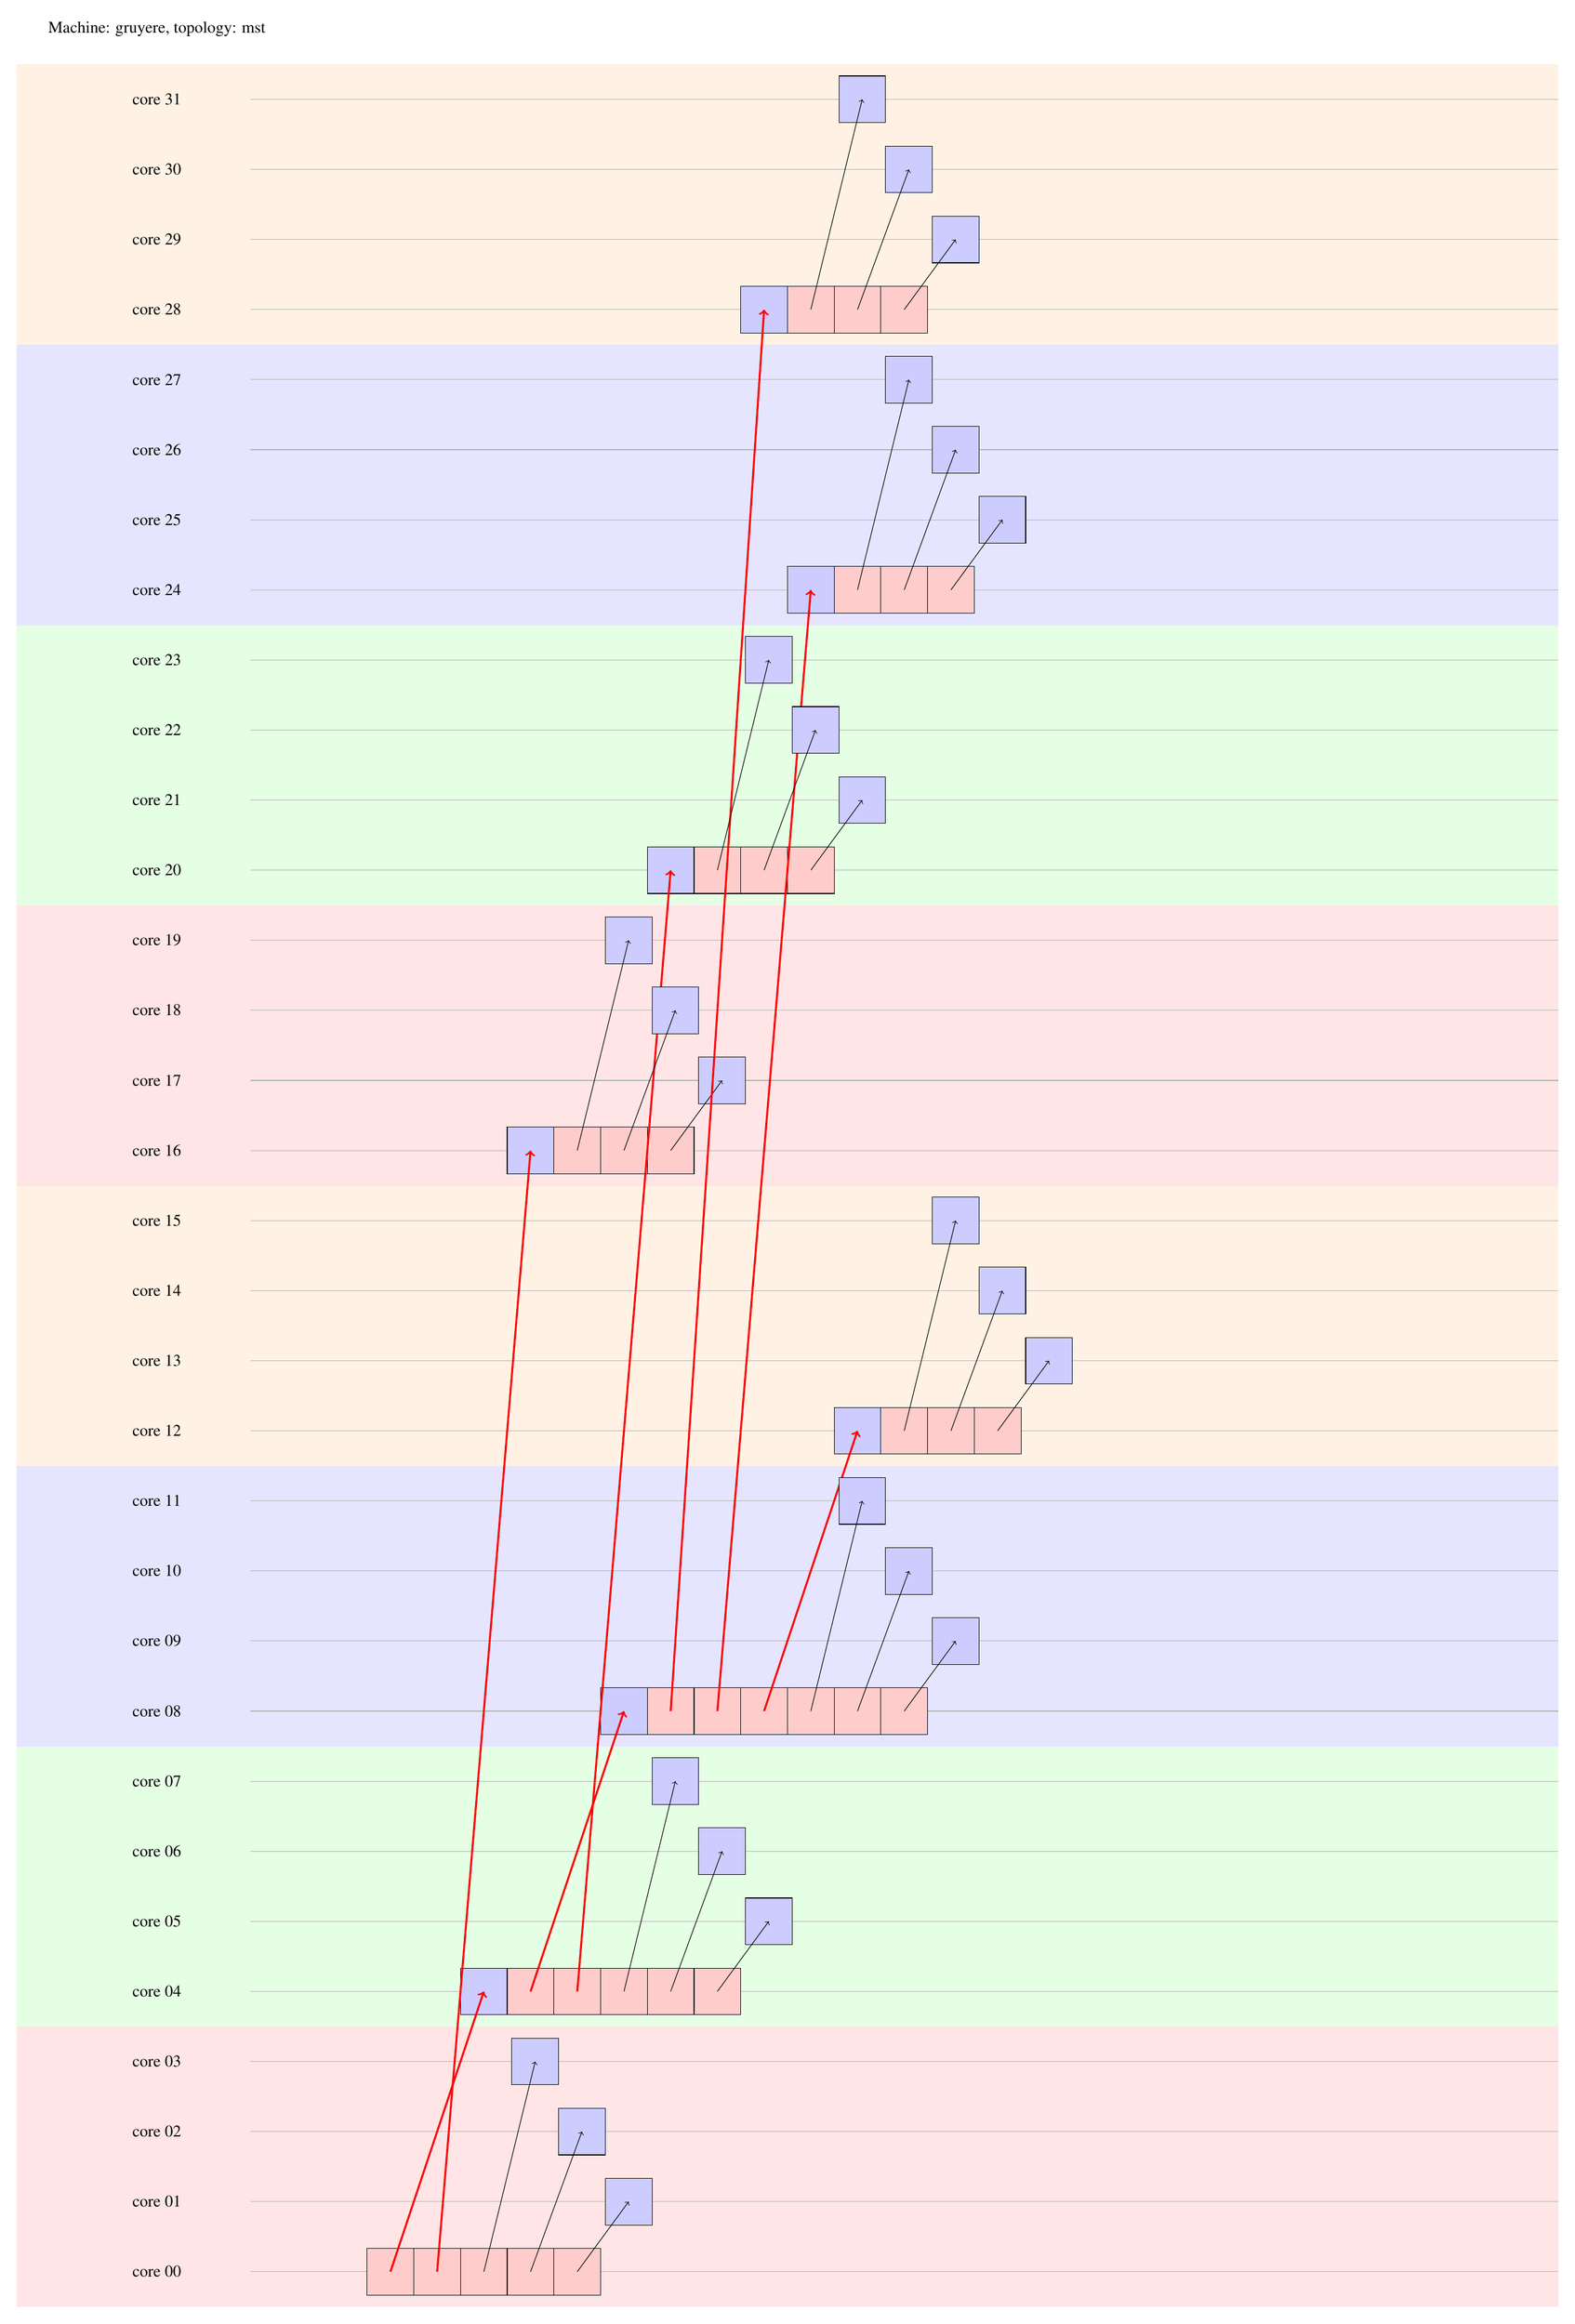
\begin{tikzpicture}[]
  % Insert visualization
  \draw[fill,color=red!10] (-3cm,7.500000mm) rectangle (30cm,-7.500000mm);
\node at (0mm,0mm) {core 00};
\draw[color=black!30] (20mm,0mm) -- (30cm,0mm);
\draw[fill,color=red!10] (-3cm,22.500000mm) rectangle (30cm,7.500000mm);
\node at (0mm,15mm) {core 01};
\draw[color=black!30] (20mm,15mm) -- (30cm,15mm);
\draw[fill,color=red!10] (-3cm,37.500000mm) rectangle (30cm,22.500000mm);
\node at (0mm,30mm) {core 02};
\draw[color=black!30] (20mm,30mm) -- (30cm,30mm);
\draw[fill,color=red!10] (-3cm,52.500000mm) rectangle (30cm,37.500000mm);
\node at (0mm,45mm) {core 03};
\draw[color=black!30] (20mm,45mm) -- (30cm,45mm);
\draw[fill,color=green!10] (-3cm,67.500000mm) rectangle (30cm,52.500000mm);
\node at (0mm,60mm) {core 04};
\draw[color=black!30] (20mm,60mm) -- (30cm,60mm);
\draw[fill,color=green!10] (-3cm,82.500000mm) rectangle (30cm,67.500000mm);
\node at (0mm,75mm) {core 05};
\draw[color=black!30] (20mm,75mm) -- (30cm,75mm);
\draw[fill,color=green!10] (-3cm,97.500000mm) rectangle (30cm,82.500000mm);
\node at (0mm,90mm) {core 06};
\draw[color=black!30] (20mm,90mm) -- (30cm,90mm);
\draw[fill,color=green!10] (-3cm,112.500000mm) rectangle (30cm,97.500000mm);
\node at (0mm,105mm) {core 07};
\draw[color=black!30] (20mm,105mm) -- (30cm,105mm);
\draw[fill,color=blue!10] (-3cm,127.500000mm) rectangle (30cm,112.500000mm);
\node at (0mm,120mm) {core 08};
\draw[color=black!30] (20mm,120mm) -- (30cm,120mm);
\draw[fill,color=blue!10] (-3cm,142.500000mm) rectangle (30cm,127.500000mm);
\node at (0mm,135mm) {core 09};
\draw[color=black!30] (20mm,135mm) -- (30cm,135mm);
\draw[fill,color=blue!10] (-3cm,157.500000mm) rectangle (30cm,142.500000mm);
\node at (0mm,150mm) {core 10};
\draw[color=black!30] (20mm,150mm) -- (30cm,150mm);
\draw[fill,color=blue!10] (-3cm,172.500000mm) rectangle (30cm,157.500000mm);
\node at (0mm,165mm) {core 11};
\draw[color=black!30] (20mm,165mm) -- (30cm,165mm);
\draw[fill,color=orange!10] (-3cm,187.500000mm) rectangle (30cm,172.500000mm);
\node at (0mm,180mm) {core 12};
\draw[color=black!30] (20mm,180mm) -- (30cm,180mm);
\draw[fill,color=orange!10] (-3cm,202.500000mm) rectangle (30cm,187.500000mm);
\node at (0mm,195mm) {core 13};
\draw[color=black!30] (20mm,195mm) -- (30cm,195mm);
\draw[fill,color=orange!10] (-3cm,217.500000mm) rectangle (30cm,202.500000mm);
\node at (0mm,210mm) {core 14};
\draw[color=black!30] (20mm,210mm) -- (30cm,210mm);
\draw[fill,color=orange!10] (-3cm,232.500000mm) rectangle (30cm,217.500000mm);
\node at (0mm,225mm) {core 15};
\draw[color=black!30] (20mm,225mm) -- (30cm,225mm);
\draw[fill,color=red!10] (-3cm,247.500000mm) rectangle (30cm,232.500000mm);
\node at (0mm,240mm) {core 16};
\draw[color=black!30] (20mm,240mm) -- (30cm,240mm);
\draw[fill,color=red!10] (-3cm,262.500000mm) rectangle (30cm,247.500000mm);
\node at (0mm,255mm) {core 17};
\draw[color=black!30] (20mm,255mm) -- (30cm,255mm);
\draw[fill,color=red!10] (-3cm,277.500000mm) rectangle (30cm,262.500000mm);
\node at (0mm,270mm) {core 18};
\draw[color=black!30] (20mm,270mm) -- (30cm,270mm);
\draw[fill,color=red!10] (-3cm,292.500000mm) rectangle (30cm,277.500000mm);
\node at (0mm,285mm) {core 19};
\draw[color=black!30] (20mm,285mm) -- (30cm,285mm);
\draw[fill,color=green!10] (-3cm,307.500000mm) rectangle (30cm,292.500000mm);
\node at (0mm,300mm) {core 20};
\draw[color=black!30] (20mm,300mm) -- (30cm,300mm);
\draw[fill,color=green!10] (-3cm,322.500000mm) rectangle (30cm,307.500000mm);
\node at (0mm,315mm) {core 21};
\draw[color=black!30] (20mm,315mm) -- (30cm,315mm);
\draw[fill,color=green!10] (-3cm,337.500000mm) rectangle (30cm,322.500000mm);
\node at (0mm,330mm) {core 22};
\draw[color=black!30] (20mm,330mm) -- (30cm,330mm);
\draw[fill,color=green!10] (-3cm,352.500000mm) rectangle (30cm,337.500000mm);
\node at (0mm,345mm) {core 23};
\draw[color=black!30] (20mm,345mm) -- (30cm,345mm);
\draw[fill,color=blue!10] (-3cm,367.500000mm) rectangle (30cm,352.500000mm);
\node at (0mm,360mm) {core 24};
\draw[color=black!30] (20mm,360mm) -- (30cm,360mm);
\draw[fill,color=blue!10] (-3cm,382.500000mm) rectangle (30cm,367.500000mm);
\node at (0mm,375mm) {core 25};
\draw[color=black!30] (20mm,375mm) -- (30cm,375mm);
\draw[fill,color=blue!10] (-3cm,397.500000mm) rectangle (30cm,382.500000mm);
\node at (0mm,390mm) {core 26};
\draw[color=black!30] (20mm,390mm) -- (30cm,390mm);
\draw[fill,color=blue!10] (-3cm,412.500000mm) rectangle (30cm,397.500000mm);
\node at (0mm,405mm) {core 27};
\draw[color=black!30] (20mm,405mm) -- (30cm,405mm);
\draw[fill,color=orange!10] (-3cm,427.500000mm) rectangle (30cm,412.500000mm);
\node at (0mm,420mm) {core 28};
\draw[color=black!30] (20mm,420mm) -- (30cm,420mm);
\draw[fill,color=orange!10] (-3cm,442.500000mm) rectangle (30cm,427.500000mm);
\node at (0mm,435mm) {core 29};
\draw[color=black!30] (20mm,435mm) -- (30cm,435mm);
\draw[fill,color=orange!10] (-3cm,457.500000mm) rectangle (30cm,442.500000mm);
\node at (0mm,450mm) {core 30};
\draw[color=black!30] (20mm,450mm) -- (30cm,450mm);
\draw[fill,color=orange!10] (-3cm,472.500000mm) rectangle (30cm,457.500000mm);
\node at (0mm,465mm) {core 31};
\draw[color=black!30] (20mm,465mm) -- (30cm,465mm);
\node at (0mm,480mm) {Machine: gruyere, topology: mst};
\node[draw,fill=red!20,minimum size=10mm] (s_0_4) at (50mm,0mm) {};
\node[draw,fill=red!20,minimum size=10mm] (s_0_16) at (60mm,0mm) {};
\node[draw,fill=red!20,minimum size=10mm] (s_0_3) at (70mm,0mm) {};
\node[draw,fill=red!20,minimum size=10mm] (s_0_2) at (80mm,0mm) {};
\node[draw,fill=red!20,minimum size=10mm] (s_0_1) at (90mm,0mm) {};
\node[draw,fill=blue!20,minimum size=10mm] (r_0_4) at (70mm,60mm) {};
\draw[->,very thick,color=red] (s_0_4.center) -- (r_0_4.center); 
\node[draw,fill=red!20,minimum size=10mm] (s_4_8) at (80mm,60mm) {};
\node[draw,fill=red!20,minimum size=10mm] (s_4_20) at (90mm,60mm) {};
\node[draw,fill=red!20,minimum size=10mm] (s_4_7) at (100mm,60mm) {};
\node[draw,fill=red!20,minimum size=10mm] (s_4_6) at (110mm,60mm) {};
\node[draw,fill=red!20,minimum size=10mm] (s_4_5) at (120mm,60mm) {};
\node[draw,fill=blue!20,minimum size=10mm] (r_0_16) at (80mm,240mm) {};
\draw[->,very thick,color=red] (s_0_16.center) -- (r_0_16.center); 
\node[draw,fill=red!20,minimum size=10mm] (s_16_19) at (90mm,240mm) {};
\node[draw,fill=red!20,minimum size=10mm] (s_16_18) at (100mm,240mm) {};
\node[draw,fill=red!20,minimum size=10mm] (s_16_17) at (110mm,240mm) {};
\node[draw,fill=blue!20,minimum size=10mm] (r_0_3) at (81mm,45mm) {};
\draw[->] (s_0_3.center) -- (r_0_3.center); 
\node[draw,fill=blue!20,minimum size=10mm] (r_0_2) at (91mm,30mm) {};
\draw[->] (s_0_2.center) -- (r_0_2.center); 
\node[draw,fill=blue!20,minimum size=10mm] (r_4_8) at (100mm,120mm) {};
\draw[->,very thick,color=red] (s_4_8.center) -- (r_4_8.center); 
\node[draw,fill=red!20,minimum size=10mm] (s_8_28) at (110mm,120mm) {};
\node[draw,fill=red!20,minimum size=10mm] (s_8_24) at (120mm,120mm) {};
\node[draw,fill=red!20,minimum size=10mm] (s_8_12) at (130mm,120mm) {};
\node[draw,fill=red!20,minimum size=10mm] (s_8_11) at (140mm,120mm) {};
\node[draw,fill=red!20,minimum size=10mm] (s_8_10) at (150mm,120mm) {};
\node[draw,fill=red!20,minimum size=10mm] (s_8_9) at (160mm,120mm) {};
\node[draw,fill=blue!20,minimum size=10mm] (r_0_1) at (101mm,15mm) {};
\draw[->] (s_0_1.center) -- (r_0_1.center); 
\node[draw,fill=blue!20,minimum size=10mm] (r_16_19) at (101mm,285mm) {};
\draw[->] (s_16_19.center) -- (r_16_19.center); 
\node[draw,fill=blue!20,minimum size=10mm] (r_4_20) at (110mm,300mm) {};
\draw[->,very thick,color=red] (s_4_20.center) -- (r_4_20.center); 
\node[draw,fill=red!20,minimum size=10mm] (s_20_23) at (120mm,300mm) {};
\node[draw,fill=red!20,minimum size=10mm] (s_20_22) at (130mm,300mm) {};
\node[draw,fill=red!20,minimum size=10mm] (s_20_21) at (140mm,300mm) {};
\node[draw,fill=blue!20,minimum size=10mm] (r_4_7) at (111mm,105mm) {};
\draw[->] (s_4_7.center) -- (r_4_7.center); 
\node[draw,fill=blue!20,minimum size=10mm] (r_16_18) at (111mm,270mm) {};
\draw[->] (s_16_18.center) -- (r_16_18.center); 
\node[draw,fill=blue!20,minimum size=10mm] (r_16_17) at (121mm,255mm) {};
\draw[->] (s_16_17.center) -- (r_16_17.center); 
\node[draw,fill=blue!20,minimum size=10mm] (r_4_6) at (121mm,90mm) {};
\draw[->] (s_4_6.center) -- (r_4_6.center); 
\node[draw,fill=blue!20,minimum size=10mm] (r_8_28) at (130mm,420mm) {};
\draw[->,very thick,color=red] (s_8_28.center) -- (r_8_28.center); 
\node[draw,fill=red!20,minimum size=10mm] (s_28_31) at (140mm,420mm) {};
\node[draw,fill=red!20,minimum size=10mm] (s_28_30) at (150mm,420mm) {};
\node[draw,fill=red!20,minimum size=10mm] (s_28_29) at (160mm,420mm) {};
\node[draw,fill=blue!20,minimum size=10mm] (r_20_23) at (131mm,345mm) {};
\draw[->] (s_20_23.center) -- (r_20_23.center); 
\node[draw,fill=blue!20,minimum size=10mm] (r_4_5) at (131mm,75mm) {};
\draw[->] (s_4_5.center) -- (r_4_5.center); 
\node[draw,fill=blue!20,minimum size=10mm] (r_8_24) at (140mm,360mm) {};
\draw[->,very thick,color=red] (s_8_24.center) -- (r_8_24.center); 
\node[draw,fill=red!20,minimum size=10mm] (s_24_27) at (150mm,360mm) {};
\node[draw,fill=red!20,minimum size=10mm] (s_24_26) at (160mm,360mm) {};
\node[draw,fill=red!20,minimum size=10mm] (s_24_25) at (170mm,360mm) {};
\node[draw,fill=blue!20,minimum size=10mm] (r_20_22) at (141mm,330mm) {};
\draw[->] (s_20_22.center) -- (r_20_22.center); 
\node[draw,fill=blue!20,minimum size=10mm] (r_8_12) at (150mm,180mm) {};
\draw[->,very thick,color=red] (s_8_12.center) -- (r_8_12.center); 
\node[draw,fill=red!20,minimum size=10mm] (s_12_15) at (160mm,180mm) {};
\node[draw,fill=red!20,minimum size=10mm] (s_12_14) at (170mm,180mm) {};
\node[draw,fill=red!20,minimum size=10mm] (s_12_13) at (180mm,180mm) {};
\node[draw,fill=blue!20,minimum size=10mm] (r_8_11) at (151mm,165mm) {};
\draw[->] (s_8_11.center) -- (r_8_11.center); 
\node[draw,fill=blue!20,minimum size=10mm] (r_28_31) at (151mm,465mm) {};
\draw[->] (s_28_31.center) -- (r_28_31.center); 
\node[draw,fill=blue!20,minimum size=10mm] (r_20_21) at (151mm,315mm) {};
\draw[->] (s_20_21.center) -- (r_20_21.center); 
\node[draw,fill=blue!20,minimum size=10mm] (r_28_30) at (161mm,450mm) {};
\draw[->] (s_28_30.center) -- (r_28_30.center); 
\node[draw,fill=blue!20,minimum size=10mm] (r_24_27) at (161mm,405mm) {};
\draw[->] (s_24_27.center) -- (r_24_27.center); 
\node[draw,fill=blue!20,minimum size=10mm] (r_8_10) at (161mm,150mm) {};
\draw[->] (s_8_10.center) -- (r_8_10.center); 
\node[draw,fill=blue!20,minimum size=10mm] (r_12_15) at (171mm,225mm) {};
\draw[->] (s_12_15.center) -- (r_12_15.center); 
\node[draw,fill=blue!20,minimum size=10mm] (r_24_26) at (171mm,390mm) {};
\draw[->] (s_24_26.center) -- (r_24_26.center); 
\node[draw,fill=blue!20,minimum size=10mm] (r_28_29) at (171mm,435mm) {};
\draw[->] (s_28_29.center) -- (r_28_29.center); 
\node[draw,fill=blue!20,minimum size=10mm] (r_8_9) at (171mm,135mm) {};
\draw[->] (s_8_9.center) -- (r_8_9.center); 
\node[draw,fill=blue!20,minimum size=10mm] (r_12_14) at (181mm,210mm) {};
\draw[->] (s_12_14.center) -- (r_12_14.center); 
\node[draw,fill=blue!20,minimum size=10mm] (r_24_25) at (181mm,375mm) {};
\draw[->] (s_24_25.center) -- (r_24_25.center); 
\node[draw,fill=blue!20,minimum size=10mm] (r_12_13) at (191mm,195mm) {};
\draw[->] (s_12_13.center) -- (r_12_13.center); 

\end{tikzpicture}
\newpage
\subsubsection{bintree}
\begin{tikzpicture}[]
  % Insert visualization
  \input{graphs/visu_gruyere_bintree}
\end{tikzpicture}
\newpage
\subsubsection{sequential}
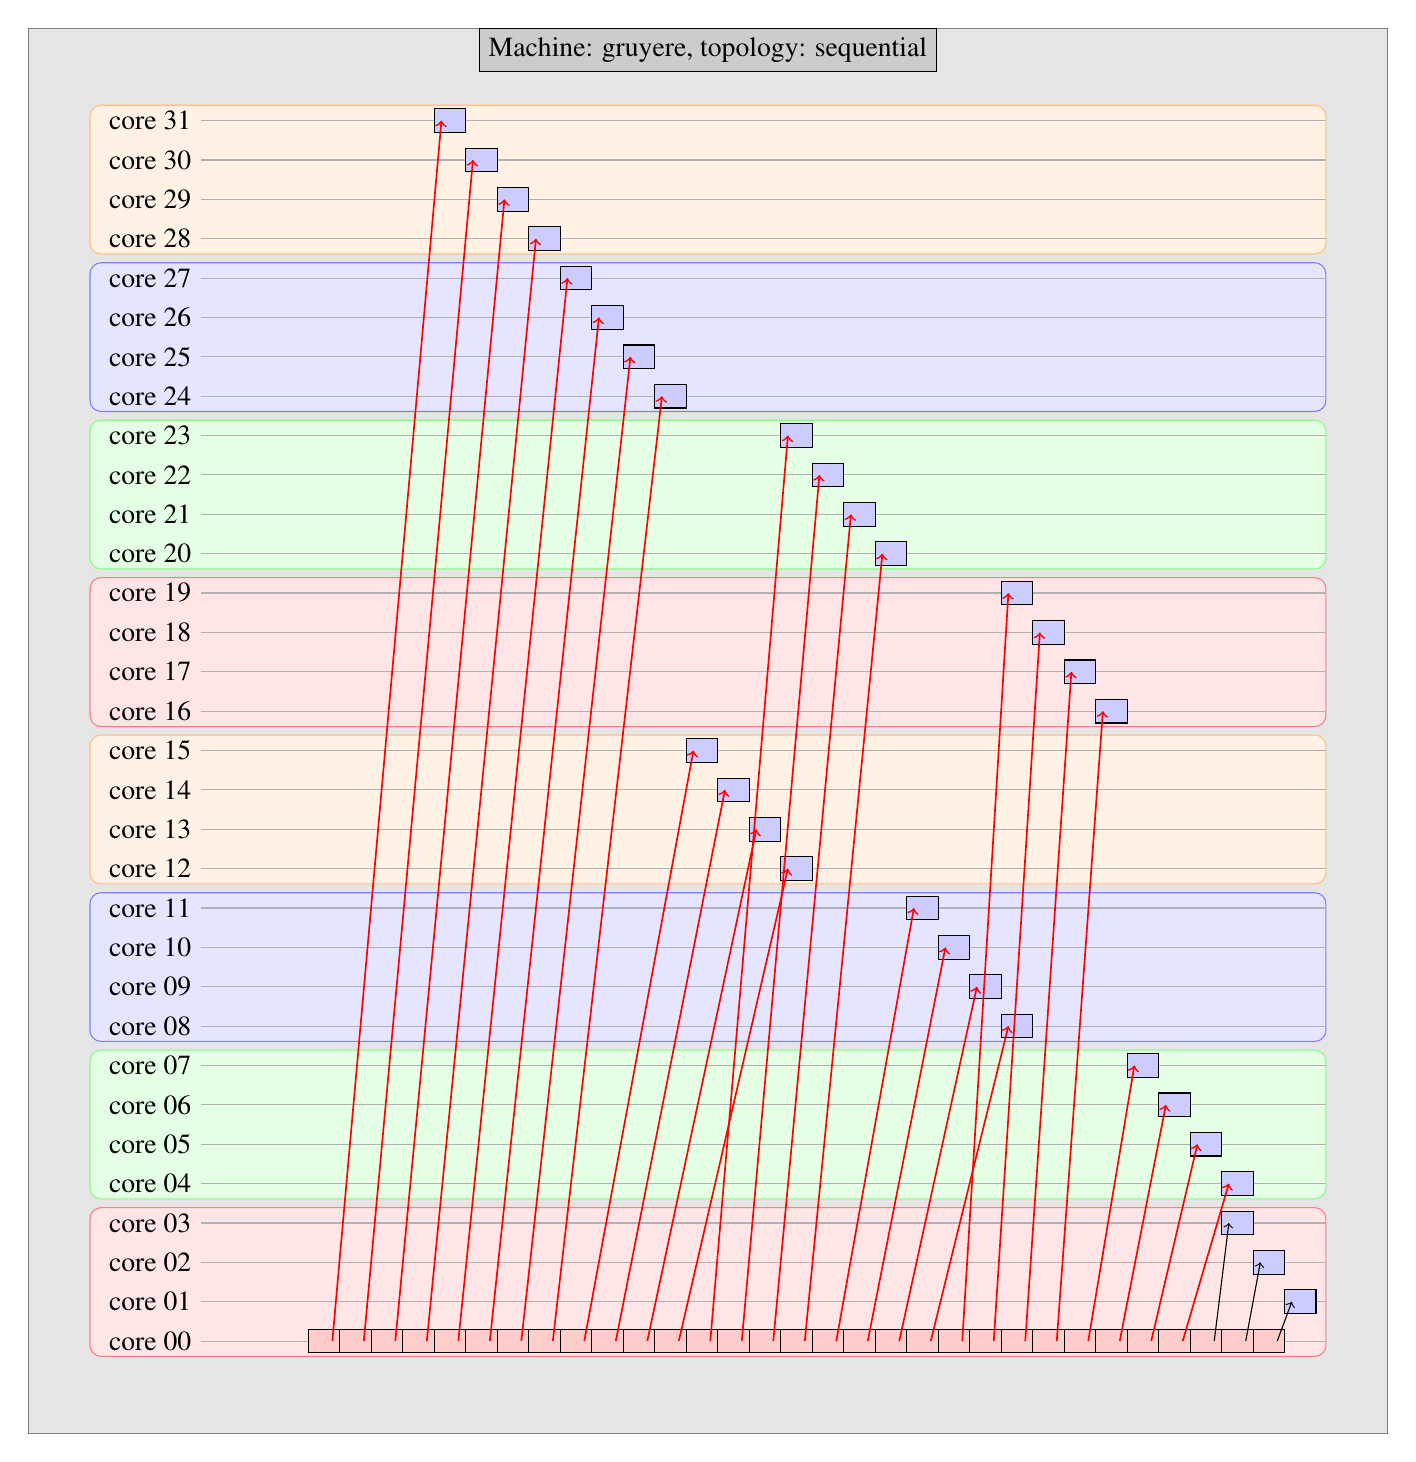
\begin{tikzpicture}[]
  % Insert visualization
  \node (core_0_label) at (0mm,0mm) {core 00};
\node (core_1_label) at (0mm,5mm) {core 01};
\node (core_2_label) at (0mm,10mm) {core 02};
\node (core_3_label) at (0mm,15mm) {core 03};
\node (core_4_label) at (0mm,20mm) {core 04};
\node (core_5_label) at (0mm,25mm) {core 05};
\node (core_6_label) at (0mm,30mm) {core 06};
\node (core_7_label) at (0mm,35mm) {core 07};
\node (core_8_label) at (0mm,40mm) {core 08};
\node (core_9_label) at (0mm,45mm) {core 09};
\node (core_10_label) at (0mm,50mm) {core 10};
\node (core_11_label) at (0mm,55mm) {core 11};
\node (core_12_label) at (0mm,60mm) {core 12};
\node (core_13_label) at (0mm,65mm) {core 13};
\node (core_14_label) at (0mm,70mm) {core 14};
\node (core_15_label) at (0mm,75mm) {core 15};
\node (core_16_label) at (0mm,80mm) {core 16};
\node (core_17_label) at (0mm,85mm) {core 17};
\node (core_18_label) at (0mm,90mm) {core 18};
\node (core_19_label) at (0mm,95mm) {core 19};
\node (core_20_label) at (0mm,100mm) {core 20};
\node (core_21_label) at (0mm,105mm) {core 21};
\node (core_22_label) at (0mm,110mm) {core 22};
\node (core_23_label) at (0mm,115mm) {core 23};
\node (core_24_label) at (0mm,120mm) {core 24};
\node (core_25_label) at (0mm,125mm) {core 25};
\node (core_26_label) at (0mm,130mm) {core 26};
\node (core_27_label) at (0mm,135mm) {core 27};
\node (core_28_label) at (0mm,140mm) {core 28};
\node (core_29_label) at (0mm,145mm) {core 29};
\node (core_30_label) at (0mm,150mm) {core 30};
\node (core_31_label) at (0mm,155mm) {core 31};
\node[draw,fill=red!20,minimum width=4mm, minimum height=3mm,anchor=west] (s_0_31) at (20mm,0mm) {};
\node[draw,fill=red!20,minimum width=4mm, minimum height=3mm,anchor=west] (s_0_30) at (24mm,0mm) {};
\node[draw,fill=red!20,minimum width=4mm, minimum height=3mm,anchor=west] (s_0_29) at (28mm,0mm) {};
\node[draw,fill=red!20,minimum width=4mm, minimum height=3mm,anchor=west] (s_0_28) at (32mm,0mm) {};
\node[draw,fill=red!20,minimum width=4mm, minimum height=3mm,anchor=west] (s_0_27) at (36mm,0mm) {};
\node[draw,fill=red!20,minimum width=4mm, minimum height=3mm,anchor=west] (s_0_26) at (40mm,0mm) {};
\node[draw,fill=red!20,minimum width=4mm, minimum height=3mm,anchor=west] (s_0_25) at (44mm,0mm) {};
\node[draw,fill=red!20,minimum width=4mm, minimum height=3mm,anchor=west] (s_0_24) at (48mm,0mm) {};
\node[draw,fill=red!20,minimum width=4mm, minimum height=3mm,anchor=west] (s_0_15) at (52mm,0mm) {};
\node[draw,fill=red!20,minimum width=4mm, minimum height=3mm,anchor=west] (s_0_14) at (56mm,0mm) {};
\node[draw,fill=red!20,minimum width=4mm, minimum height=3mm,anchor=west] (s_0_13) at (60mm,0mm) {};
\node[draw,fill=red!20,minimum width=4mm, minimum height=3mm,anchor=west] (s_0_12) at (64mm,0mm) {};
\node[draw,fill=red!20,minimum width=4mm, minimum height=3mm,anchor=west] (s_0_23) at (68mm,0mm) {};
\node[draw,fill=red!20,minimum width=4mm, minimum height=3mm,anchor=west] (s_0_22) at (72mm,0mm) {};
\node[draw,fill=red!20,minimum width=4mm, minimum height=3mm,anchor=west] (s_0_21) at (76mm,0mm) {};
\node[draw,fill=red!20,minimum width=4mm, minimum height=3mm,anchor=west] (s_0_20) at (80mm,0mm) {};
\node[draw,fill=red!20,minimum width=4mm, minimum height=3mm,anchor=west] (s_0_11) at (84mm,0mm) {};
\node[draw,fill=red!20,minimum width=4mm, minimum height=3mm,anchor=west] (s_0_10) at (88mm,0mm) {};
\node[draw,fill=red!20,minimum width=4mm, minimum height=3mm,anchor=west] (s_0_9) at (92mm,0mm) {};
\node[draw,fill=red!20,minimum width=4mm, minimum height=3mm,anchor=west] (s_0_8) at (96mm,0mm) {};
\node[draw,fill=red!20,minimum width=4mm, minimum height=3mm,anchor=west] (s_0_19) at (100mm,0mm) {};
\node[draw,fill=red!20,minimum width=4mm, minimum height=3mm,anchor=west] (s_0_18) at (104mm,0mm) {};
\node[draw,fill=red!20,minimum width=4mm, minimum height=3mm,anchor=west] (s_0_17) at (108mm,0mm) {};
\node[draw,fill=red!20,minimum width=4mm, minimum height=3mm,anchor=west] (s_0_16) at (112mm,0mm) {};
\node[draw,fill=red!20,minimum width=4mm, minimum height=3mm,anchor=west] (s_0_7) at (116mm,0mm) {};
\node[draw,fill=red!20,minimum width=4mm, minimum height=3mm,anchor=west] (s_0_6) at (120mm,0mm) {};
\node[draw,fill=red!20,minimum width=4mm, minimum height=3mm,anchor=west] (s_0_5) at (124mm,0mm) {};
\node[draw,fill=red!20,minimum width=4mm, minimum height=3mm,anchor=west] (s_0_4) at (128mm,0mm) {};
\node[draw,fill=red!20,minimum width=4mm, minimum height=3mm,anchor=west] (s_0_3) at (132mm,0mm) {};
\node[draw,fill=red!20,minimum width=4mm, minimum height=3mm,anchor=west] (s_0_2) at (136mm,0mm) {};
\node[draw,fill=red!20,minimum width=4mm, minimum height=3mm,anchor=west] (s_0_1) at (140mm,0mm) {};
\node[draw,fill=blue!20,minimum width=4mm, minimum height=3mm,anchor=west] (r_0_31) at (36mm,155mm) {};
\draw[->,semithick,color=red] ($(s_0_31.east)-(1mm,0mm)$) -- ($(r_0_31.west)+(1mm,0mm)$); 
\node[draw,fill=blue!20,minimum width=4mm, minimum height=3mm,anchor=west] (r_0_30) at (40mm,150mm) {};
\draw[->,semithick,color=red] ($(s_0_30.east)-(1mm,0mm)$) -- ($(r_0_30.west)+(1mm,0mm)$); 
\node[draw,fill=blue!20,minimum width=4mm, minimum height=3mm,anchor=west] (r_0_29) at (44mm,145mm) {};
\draw[->,semithick,color=red] ($(s_0_29.east)-(1mm,0mm)$) -- ($(r_0_29.west)+(1mm,0mm)$); 
\node[draw,fill=blue!20,minimum width=4mm, minimum height=3mm,anchor=west] (r_0_28) at (48mm,140mm) {};
\draw[->,semithick,color=red] ($(s_0_28.east)-(1mm,0mm)$) -- ($(r_0_28.west)+(1mm,0mm)$); 
\node[draw,fill=blue!20,minimum width=4mm, minimum height=3mm,anchor=west] (r_0_27) at (52mm,135mm) {};
\draw[->,semithick,color=red] ($(s_0_27.east)-(1mm,0mm)$) -- ($(r_0_27.west)+(1mm,0mm)$); 
\node[draw,fill=blue!20,minimum width=4mm, minimum height=3mm,anchor=west] (r_0_26) at (56mm,130mm) {};
\draw[->,semithick,color=red] ($(s_0_26.east)-(1mm,0mm)$) -- ($(r_0_26.west)+(1mm,0mm)$); 
\node[draw,fill=blue!20,minimum width=4mm, minimum height=3mm,anchor=west] (r_0_25) at (60mm,125mm) {};
\draw[->,semithick,color=red] ($(s_0_25.east)-(1mm,0mm)$) -- ($(r_0_25.west)+(1mm,0mm)$); 
\node[draw,fill=blue!20,minimum width=4mm, minimum height=3mm,anchor=west] (r_0_24) at (64mm,120mm) {};
\draw[->,semithick,color=red] ($(s_0_24.east)-(1mm,0mm)$) -- ($(r_0_24.west)+(1mm,0mm)$); 
\node[draw,fill=blue!20,minimum width=4mm, minimum height=3mm,anchor=west] (r_0_15) at (68mm,75mm) {};
\draw[->,semithick,color=red] ($(s_0_15.east)-(1mm,0mm)$) -- ($(r_0_15.west)+(1mm,0mm)$); 
\node[draw,fill=blue!20,minimum width=4mm, minimum height=3mm,anchor=west] (r_0_14) at (72mm,70mm) {};
\draw[->,semithick,color=red] ($(s_0_14.east)-(1mm,0mm)$) -- ($(r_0_14.west)+(1mm,0mm)$); 
\node[draw,fill=blue!20,minimum width=4mm, minimum height=3mm,anchor=west] (r_0_13) at (76mm,65mm) {};
\draw[->,semithick,color=red] ($(s_0_13.east)-(1mm,0mm)$) -- ($(r_0_13.west)+(1mm,0mm)$); 
\node[draw,fill=blue!20,minimum width=4mm, minimum height=3mm,anchor=west] (r_0_23) at (80mm,115mm) {};
\draw[->,semithick,color=red] ($(s_0_23.east)-(1mm,0mm)$) -- ($(r_0_23.west)+(1mm,0mm)$); 
\node[draw,fill=blue!20,minimum width=4mm, minimum height=3mm,anchor=west] (r_0_12) at (80mm,60mm) {};
\draw[->,semithick,color=red] ($(s_0_12.east)-(1mm,0mm)$) -- ($(r_0_12.west)+(1mm,0mm)$); 
\node[draw,fill=blue!20,minimum width=4mm, minimum height=3mm,anchor=west] (r_0_22) at (84mm,110mm) {};
\draw[->,semithick,color=red] ($(s_0_22.east)-(1mm,0mm)$) -- ($(r_0_22.west)+(1mm,0mm)$); 
\node[draw,fill=blue!20,minimum width=4mm, minimum height=3mm,anchor=west] (r_0_21) at (88mm,105mm) {};
\draw[->,semithick,color=red] ($(s_0_21.east)-(1mm,0mm)$) -- ($(r_0_21.west)+(1mm,0mm)$); 
\node[draw,fill=blue!20,minimum width=4mm, minimum height=3mm,anchor=west] (r_0_20) at (92mm,100mm) {};
\draw[->,semithick,color=red] ($(s_0_20.east)-(1mm,0mm)$) -- ($(r_0_20.west)+(1mm,0mm)$); 
\node[draw,fill=blue!20,minimum width=4mm, minimum height=3mm,anchor=west] (r_0_11) at (96mm,55mm) {};
\draw[->,semithick,color=red] ($(s_0_11.east)-(1mm,0mm)$) -- ($(r_0_11.west)+(1mm,0mm)$); 
\node[draw,fill=blue!20,minimum width=4mm, minimum height=3mm,anchor=west] (r_0_10) at (100mm,50mm) {};
\draw[->,semithick,color=red] ($(s_0_10.east)-(1mm,0mm)$) -- ($(r_0_10.west)+(1mm,0mm)$); 
\node[draw,fill=blue!20,minimum width=4mm, minimum height=3mm,anchor=west] (r_0_9) at (104mm,45mm) {};
\draw[->,semithick,color=red] ($(s_0_9.east)-(1mm,0mm)$) -- ($(r_0_9.west)+(1mm,0mm)$); 
\node[draw,fill=blue!20,minimum width=4mm, minimum height=3mm,anchor=west] (r_0_19) at (108mm,95mm) {};
\draw[->,semithick,color=red] ($(s_0_19.east)-(1mm,0mm)$) -- ($(r_0_19.west)+(1mm,0mm)$); 
\node[draw,fill=blue!20,minimum width=4mm, minimum height=3mm,anchor=west] (r_0_8) at (108mm,40mm) {};
\draw[->,semithick,color=red] ($(s_0_8.east)-(1mm,0mm)$) -- ($(r_0_8.west)+(1mm,0mm)$); 
\node[draw,fill=blue!20,minimum width=4mm, minimum height=3mm,anchor=west] (r_0_18) at (112mm,90mm) {};
\draw[->,semithick,color=red] ($(s_0_18.east)-(1mm,0mm)$) -- ($(r_0_18.west)+(1mm,0mm)$); 
\node[draw,fill=blue!20,minimum width=4mm, minimum height=3mm,anchor=west] (r_0_17) at (116mm,85mm) {};
\draw[->,semithick,color=red] ($(s_0_17.east)-(1mm,0mm)$) -- ($(r_0_17.west)+(1mm,0mm)$); 
\node[draw,fill=blue!20,minimum width=4mm, minimum height=3mm,anchor=west] (r_0_16) at (120mm,80mm) {};
\draw[->,semithick,color=red] ($(s_0_16.east)-(1mm,0mm)$) -- ($(r_0_16.west)+(1mm,0mm)$); 
\node[draw,fill=blue!20,minimum width=4mm, minimum height=3mm,anchor=west] (r_0_7) at (124mm,35mm) {};
\draw[->,semithick,color=red] ($(s_0_7.east)-(1mm,0mm)$) -- ($(r_0_7.west)+(1mm,0mm)$); 
\node[draw,fill=blue!20,minimum width=4mm, minimum height=3mm,anchor=west] (r_0_6) at (128mm,30mm) {};
\draw[->,semithick,color=red] ($(s_0_6.east)-(1mm,0mm)$) -- ($(r_0_6.west)+(1mm,0mm)$); 
\node[draw,fill=blue!20,minimum width=4mm, minimum height=3mm,anchor=west] (r_0_5) at (132mm,25mm) {};
\draw[->,semithick,color=red] ($(s_0_5.east)-(1mm,0mm)$) -- ($(r_0_5.west)+(1mm,0mm)$); 
\node[draw,fill=blue!20,minimum width=4mm, minimum height=3mm,anchor=west] (r_0_4) at (136mm,20mm) {};
\draw[->,semithick,color=red] ($(s_0_4.east)-(1mm,0mm)$) -- ($(r_0_4.west)+(1mm,0mm)$); 
\node[draw,fill=blue!20,minimum width=4mm, minimum height=3mm,anchor=west] (r_0_3) at (136mm,15mm) {};
\draw[->] ($(s_0_3.east)-(1mm,0mm)$) -- ($(r_0_3.west)+(1mm,0mm)$); 
\node[draw,fill=blue!20,minimum width=4mm, minimum height=3mm,anchor=west] (r_0_2) at (140mm,10mm) {};
\draw[->] ($(s_0_2.east)-(1mm,0mm)$) -- ($(r_0_2.west)+(1mm,0mm)$); 
\node[draw,fill=blue!20,minimum width=4mm, minimum height=3mm,anchor=west] (r_0_1) at (144mm,5mm) {};
\draw[->] ($(s_0_1.east)-(1mm,0mm)$) -- ($(r_0_1.west)+(1mm,0mm)$); 
\begin{pgfonlayer}{background}
\node [fit=(core_0_label) (core_1_label) (core_2_label) (core_3_label) (core_4_label) (core_5_label) (core_6_label) (core_7_label) (core_8_label) (core_9_label) (core_10_label) (core_11_label) (core_12_label) (core_13_label) (core_14_label) (core_15_label) (core_16_label) (core_17_label) (core_18_label) (core_19_label) (core_20_label) (core_21_label) (core_22_label) (core_23_label) (core_24_label) (core_25_label) (core_26_label) (core_27_label) (core_28_label) (core_29_label) (core_30_label) (core_31_label) (s_0_31) (s_0_30) (s_0_29) (s_0_28) (s_0_27) (s_0_26) (s_0_25) (s_0_24) (s_0_15) (s_0_14) (s_0_13) (s_0_12) (s_0_23) (s_0_22) (s_0_21) (s_0_20) (s_0_11) (s_0_10) (s_0_9) (s_0_8) (s_0_19) (s_0_18) (s_0_17) (s_0_16) (s_0_7) (s_0_6) (s_0_5) (s_0_4) (s_0_3) (s_0_2) (s_0_1) (r_0_31) (r_0_30) (r_0_29) (r_0_28) (r_0_27) (r_0_26) (r_0_25) (r_0_24) (r_0_15) (r_0_14) (r_0_13) (r_0_12) (r_0_23) (r_0_22) (r_0_21) (r_0_20) (r_0_11) (r_0_10) (r_0_9) (r_0_8) (r_0_19) (r_0_18) (r_0_17) (r_0_16) (r_0_7) (r_0_6) (r_0_5) (r_0_4) (r_0_3) (r_0_2) (r_0_1) (core_0_label) (core_1_label) (core_2_label) (core_3_label) (core_4_label) (core_5_label) (core_6_label) (core_7_label) (core_8_label) (core_9_label) (core_10_label) (core_11_label) (core_12_label) (core_13_label) (core_14_label) (core_15_label) (core_16_label) (core_17_label) (core_18_label) (core_19_label) (core_20_label) (core_21_label) (core_22_label) (core_23_label) (core_24_label) (core_25_label) (core_26_label) (core_27_label) (core_28_label) (core_29_label) (core_30_label) (core_31_label) (s_0_31) (s_0_30) (s_0_29) (s_0_28) (s_0_27) (s_0_26) (s_0_25) (s_0_24) (s_0_15) (s_0_14) (s_0_13) (s_0_12) (s_0_23) (s_0_22) (s_0_21) (s_0_20) (s_0_11) (s_0_10) (s_0_9) (s_0_8) (s_0_19) (s_0_18) (s_0_17) (s_0_16) (s_0_7) (s_0_6) (s_0_5) (s_0_4) (s_0_3) (s_0_2) (s_0_1) (r_0_31) (r_0_30) (r_0_29) (r_0_28) (r_0_27) (r_0_26) (r_0_25) (r_0_24) (r_0_15) (r_0_14) (r_0_13) (r_0_23) (r_0_12) (r_0_22) (r_0_21) (r_0_20) (r_0_11) (r_0_10) (r_0_9) (r_0_19) (r_0_8) (r_0_18) (r_0_17) (r_0_16) (r_0_7) (r_0_6) (r_0_5) (r_0_4) (r_0_3) (r_0_2) (r_0_1)] (allobjects) {};
\node [draw=black!50,fill=black!10,fit=(core_0_label) (core_1_label) (core_2_label) (core_3_label) (core_4_label) (core_5_label) (core_6_label) (core_7_label) (core_8_label) (core_9_label) (core_10_label) (core_11_label) (core_12_label) (core_13_label) (core_14_label) (core_15_label) (core_16_label) (core_17_label) (core_18_label) (core_19_label) (core_20_label) (core_21_label) (core_22_label) (core_23_label) (core_24_label) (core_25_label) (core_26_label) (core_27_label) (core_28_label) (core_29_label) (core_30_label) (core_31_label) (s_0_31) (s_0_30) (s_0_29) (s_0_28) (s_0_27) (s_0_26) (s_0_25) (s_0_24) (s_0_15) (s_0_14) (s_0_13) (s_0_12) (s_0_23) (s_0_22) (s_0_21) (s_0_20) (s_0_11) (s_0_10) (s_0_9) (s_0_8) (s_0_19) (s_0_18) (s_0_17) (s_0_16) (s_0_7) (s_0_6) (s_0_5) (s_0_4) (s_0_3) (s_0_2) (s_0_1) (r_0_31) (r_0_30) (r_0_29) (r_0_28) (r_0_27) (r_0_26) (r_0_25) (r_0_24) (r_0_15) (r_0_14) (r_0_13) (r_0_12) (r_0_23) (r_0_22) (r_0_21) (r_0_20) (r_0_11) (r_0_10) (r_0_9) (r_0_8) (r_0_19) (r_0_18) (r_0_17) (r_0_16) (r_0_7) (r_0_6) (r_0_5) (r_0_4) (r_0_3) (r_0_2) (r_0_1) (core_0_label) (core_1_label) (core_2_label) (core_3_label) (core_4_label) (core_5_label) (core_6_label) (core_7_label) (core_8_label) (core_9_label) (core_10_label) (core_11_label) (core_12_label) (core_13_label) (core_14_label) (core_15_label) (core_16_label) (core_17_label) (core_18_label) (core_19_label) (core_20_label) (core_21_label) (core_22_label) (core_23_label) (core_24_label) (core_25_label) (core_26_label) (core_27_label) (core_28_label) (core_29_label) (core_30_label) (core_31_label) (s_0_31) (s_0_30) (s_0_29) (s_0_28) (s_0_27) (s_0_26) (s_0_25) (s_0_24) (s_0_15) (s_0_14) (s_0_13) (s_0_12) (s_0_23) (s_0_22) (s_0_21) (s_0_20) (s_0_11) (s_0_10) (s_0_9) (s_0_8) (s_0_19) (s_0_18) (s_0_17) (s_0_16) (s_0_7) (s_0_6) (s_0_5) (s_0_4) (s_0_3) (s_0_2) (s_0_1) (r_0_31) (r_0_30) (r_0_29) (r_0_28) (r_0_27) (r_0_26) (r_0_25) (r_0_24) (r_0_15) (r_0_14) (r_0_13) (r_0_23) (r_0_12) (r_0_22) (r_0_21) (r_0_20) (r_0_11) (r_0_10) (r_0_9) (r_0_19) (r_0_8) (r_0_18) (r_0_17) (r_0_16) (r_0_7) (r_0_6) (r_0_5) (r_0_4) (r_0_3) (r_0_2) (r_0_1),scale=1.1] (bg) {};
\draw let \p1 = (allobjects.east) in node[] (numa_axis_0) at (\x1,0mm) {};
\draw let \p1 = (allobjects.east) in node[] (numa_axis_1) at (\x1,5mm) {};
\draw let \p1 = (allobjects.east) in node[] (numa_axis_2) at (\x1,10mm) {};
\draw let \p1 = (allobjects.east) in node[] (numa_axis_3) at (\x1,15mm) {};
\draw let \p1 = (allobjects.east) in node[] (numa_axis_4) at (\x1,20mm) {};
\draw let \p1 = (allobjects.east) in node[] (numa_axis_5) at (\x1,25mm) {};
\draw let \p1 = (allobjects.east) in node[] (numa_axis_6) at (\x1,30mm) {};
\draw let \p1 = (allobjects.east) in node[] (numa_axis_7) at (\x1,35mm) {};
\draw let \p1 = (allobjects.east) in node[] (numa_axis_8) at (\x1,40mm) {};
\draw let \p1 = (allobjects.east) in node[] (numa_axis_9) at (\x1,45mm) {};
\draw let \p1 = (allobjects.east) in node[] (numa_axis_10) at (\x1,50mm) {};
\draw let \p1 = (allobjects.east) in node[] (numa_axis_11) at (\x1,55mm) {};
\draw let \p1 = (allobjects.east) in node[] (numa_axis_12) at (\x1,60mm) {};
\draw let \p1 = (allobjects.east) in node[] (numa_axis_13) at (\x1,65mm) {};
\draw let \p1 = (allobjects.east) in node[] (numa_axis_14) at (\x1,70mm) {};
\draw let \p1 = (allobjects.east) in node[] (numa_axis_15) at (\x1,75mm) {};
\draw let \p1 = (allobjects.east) in node[] (numa_axis_16) at (\x1,80mm) {};
\draw let \p1 = (allobjects.east) in node[] (numa_axis_17) at (\x1,85mm) {};
\draw let \p1 = (allobjects.east) in node[] (numa_axis_18) at (\x1,90mm) {};
\draw let \p1 = (allobjects.east) in node[] (numa_axis_19) at (\x1,95mm) {};
\draw let \p1 = (allobjects.east) in node[] (numa_axis_20) at (\x1,100mm) {};
\draw let \p1 = (allobjects.east) in node[] (numa_axis_21) at (\x1,105mm) {};
\draw let \p1 = (allobjects.east) in node[] (numa_axis_22) at (\x1,110mm) {};
\draw let \p1 = (allobjects.east) in node[] (numa_axis_23) at (\x1,115mm) {};
\draw let \p1 = (allobjects.east) in node[] (numa_axis_24) at (\x1,120mm) {};
\draw let \p1 = (allobjects.east) in node[] (numa_axis_25) at (\x1,125mm) {};
\draw let \p1 = (allobjects.east) in node[] (numa_axis_26) at (\x1,130mm) {};
\draw let \p1 = (allobjects.east) in node[] (numa_axis_27) at (\x1,135mm) {};
\draw let \p1 = (allobjects.east) in node[] (numa_axis_28) at (\x1,140mm) {};
\draw let \p1 = (allobjects.east) in node[] (numa_axis_29) at (\x1,145mm) {};
\draw let \p1 = (allobjects.east) in node[] (numa_axis_30) at (\x1,150mm) {};
\draw let \p1 = (allobjects.east) in node[] (numa_axis_31) at (\x1,155mm) {};
\node [yscale=0.85,draw=red!50,fill=red!10,fit=(core_0_label) (core_1_label) (core_2_label) (core_3_label) (s_0_31) (s_0_30) (s_0_29) (s_0_28) (s_0_27) (s_0_26) (s_0_25) (s_0_24) (s_0_15) (s_0_14) (s_0_13) (s_0_12) (s_0_23) (s_0_22) (s_0_21) (s_0_20) (s_0_11) (s_0_10) (s_0_9) (s_0_8) (s_0_19) (s_0_18) (s_0_17) (s_0_16) (s_0_7) (s_0_6) (s_0_5) (s_0_4) (s_0_3) (s_0_2) (s_0_1) (r_0_3) (r_0_2) (r_0_1) (numa_axis_0.west) (core_0_label) (core_1_label) (core_2_label) (core_3_label) (s_0_31) (s_0_30) (s_0_29) (s_0_28) (s_0_27) (s_0_26) (s_0_25) (s_0_24) (s_0_15) (s_0_14) (s_0_13) (s_0_12) (s_0_23) (s_0_22) (s_0_21) (s_0_20) (s_0_11) (s_0_10) (s_0_9) (s_0_8) (s_0_19) (s_0_18) (s_0_17) (s_0_16) (s_0_7) (s_0_6) (s_0_5) (s_0_4) (s_0_3) (s_0_2) (s_0_1) (r_0_3) (r_0_2) (r_0_1) (numa_axis_0.west),rounded corners] {};
\node [yscale=0.85,draw=green!50,fill=green!10,fit=(core_4_label) (core_5_label) (core_6_label) (core_7_label) (r_0_7) (r_0_6) (r_0_5) (r_0_4) (numa_axis_4.west) (core_4_label) (core_5_label) (core_6_label) (core_7_label) (r_0_7) (r_0_6) (r_0_5) (r_0_4) (numa_axis_4.west),rounded corners] {};
\node [yscale=0.85,draw=blue!50,fill=blue!10,fit=(core_8_label) (core_9_label) (core_10_label) (core_11_label) (r_0_11) (r_0_10) (r_0_9) (r_0_8) (numa_axis_8.west) (core_8_label) (core_9_label) (core_10_label) (core_11_label) (r_0_11) (r_0_10) (r_0_9) (r_0_8) (numa_axis_8.west),rounded corners] {};
\node [yscale=0.85,draw=orange!50,fill=orange!10,fit=(core_12_label) (core_13_label) (core_14_label) (core_15_label) (r_0_15) (r_0_14) (r_0_13) (r_0_12) (numa_axis_12.west) (core_12_label) (core_13_label) (core_14_label) (core_15_label) (r_0_15) (r_0_14) (r_0_13) (r_0_12) (numa_axis_12.west),rounded corners] {};
\node [yscale=0.85,draw=red!50,fill=red!10,fit=(core_16_label) (core_17_label) (core_18_label) (core_19_label) (r_0_19) (r_0_18) (r_0_17) (r_0_16) (numa_axis_16.west) (core_16_label) (core_17_label) (core_18_label) (core_19_label) (r_0_19) (r_0_18) (r_0_17) (r_0_16) (numa_axis_16.west),rounded corners] {};
\node [yscale=0.85,draw=green!50,fill=green!10,fit=(core_20_label) (core_21_label) (core_22_label) (core_23_label) (r_0_23) (r_0_22) (r_0_21) (r_0_20) (numa_axis_20.west) (core_20_label) (core_21_label) (core_22_label) (core_23_label) (r_0_23) (r_0_22) (r_0_21) (r_0_20) (numa_axis_20.west),rounded corners] {};
\node [yscale=0.85,draw=blue!50,fill=blue!10,fit=(core_24_label) (core_25_label) (core_26_label) (core_27_label) (r_0_27) (r_0_26) (r_0_25) (r_0_24) (numa_axis_24.west) (core_24_label) (core_25_label) (core_26_label) (core_27_label) (r_0_27) (r_0_26) (r_0_25) (r_0_24) (numa_axis_24.west),rounded corners] {};
\node [yscale=0.85,draw=orange!50,fill=orange!10,fit=(core_28_label) (core_29_label) (core_30_label) (core_31_label) (r_0_31) (r_0_30) (r_0_29) (r_0_28) (numa_axis_28.west) (core_28_label) (core_29_label) (core_30_label) (core_31_label) (r_0_31) (r_0_30) (r_0_29) (r_0_28) (numa_axis_28.west),rounded corners] {};
\draw[color=black!30] let \p1 = (core_10_label.east), \p2 = (allobjects.east) in (\x1,0mm) -- (\x2,0mm);
\draw[color=black!30] let \p1 = (core_10_label.east), \p2 = (allobjects.east) in (\x1,5mm) -- (\x2,5mm);
\draw[color=black!30] let \p1 = (core_10_label.east), \p2 = (allobjects.east) in (\x1,10mm) -- (\x2,10mm);
\draw[color=black!30] let \p1 = (core_10_label.east), \p2 = (allobjects.east) in (\x1,15mm) -- (\x2,15mm);
\draw[color=black!30] let \p1 = (core_10_label.east), \p2 = (allobjects.east) in (\x1,20mm) -- (\x2,20mm);
\draw[color=black!30] let \p1 = (core_10_label.east), \p2 = (allobjects.east) in (\x1,25mm) -- (\x2,25mm);
\draw[color=black!30] let \p1 = (core_10_label.east), \p2 = (allobjects.east) in (\x1,30mm) -- (\x2,30mm);
\draw[color=black!30] let \p1 = (core_10_label.east), \p2 = (allobjects.east) in (\x1,35mm) -- (\x2,35mm);
\draw[color=black!30] let \p1 = (core_10_label.east), \p2 = (allobjects.east) in (\x1,40mm) -- (\x2,40mm);
\draw[color=black!30] let \p1 = (core_10_label.east), \p2 = (allobjects.east) in (\x1,45mm) -- (\x2,45mm);
\draw[color=black!30] let \p1 = (core_10_label.east), \p2 = (allobjects.east) in (\x1,50mm) -- (\x2,50mm);
\draw[color=black!30] let \p1 = (core_10_label.east), \p2 = (allobjects.east) in (\x1,55mm) -- (\x2,55mm);
\draw[color=black!30] let \p1 = (core_10_label.east), \p2 = (allobjects.east) in (\x1,60mm) -- (\x2,60mm);
\draw[color=black!30] let \p1 = (core_10_label.east), \p2 = (allobjects.east) in (\x1,65mm) -- (\x2,65mm);
\draw[color=black!30] let \p1 = (core_10_label.east), \p2 = (allobjects.east) in (\x1,70mm) -- (\x2,70mm);
\draw[color=black!30] let \p1 = (core_10_label.east), \p2 = (allobjects.east) in (\x1,75mm) -- (\x2,75mm);
\draw[color=black!30] let \p1 = (core_10_label.east), \p2 = (allobjects.east) in (\x1,80mm) -- (\x2,80mm);
\draw[color=black!30] let \p1 = (core_10_label.east), \p2 = (allobjects.east) in (\x1,85mm) -- (\x2,85mm);
\draw[color=black!30] let \p1 = (core_10_label.east), \p2 = (allobjects.east) in (\x1,90mm) -- (\x2,90mm);
\draw[color=black!30] let \p1 = (core_10_label.east), \p2 = (allobjects.east) in (\x1,95mm) -- (\x2,95mm);
\draw[color=black!30] let \p1 = (core_10_label.east), \p2 = (allobjects.east) in (\x1,100mm) -- (\x2,100mm);
\draw[color=black!30] let \p1 = (core_10_label.east), \p2 = (allobjects.east) in (\x1,105mm) -- (\x2,105mm);
\draw[color=black!30] let \p1 = (core_10_label.east), \p2 = (allobjects.east) in (\x1,110mm) -- (\x2,110mm);
\draw[color=black!30] let \p1 = (core_10_label.east), \p2 = (allobjects.east) in (\x1,115mm) -- (\x2,115mm);
\draw[color=black!30] let \p1 = (core_10_label.east), \p2 = (allobjects.east) in (\x1,120mm) -- (\x2,120mm);
\draw[color=black!30] let \p1 = (core_10_label.east), \p2 = (allobjects.east) in (\x1,125mm) -- (\x2,125mm);
\draw[color=black!30] let \p1 = (core_10_label.east), \p2 = (allobjects.east) in (\x1,130mm) -- (\x2,130mm);
\draw[color=black!30] let \p1 = (core_10_label.east), \p2 = (allobjects.east) in (\x1,135mm) -- (\x2,135mm);
\draw[color=black!30] let \p1 = (core_10_label.east), \p2 = (allobjects.east) in (\x1,140mm) -- (\x2,140mm);
\draw[color=black!30] let \p1 = (core_10_label.east), \p2 = (allobjects.east) in (\x1,145mm) -- (\x2,145mm);
\draw[color=black!30] let \p1 = (core_10_label.east), \p2 = (allobjects.east) in (\x1,150mm) -- (\x2,150mm);
\draw[color=black!30] let \p1 = (core_10_label.east), \p2 = (allobjects.east) in (\x1,155mm) -- (\x2,155mm);
\node[draw=black,anchor=north,fill=black!20] at (bg.north) {Machine: gruyere, topology: sequential};
\end{pgfonlayer}

\end{tikzpicture}
\newpage
\subsubsection{ring}
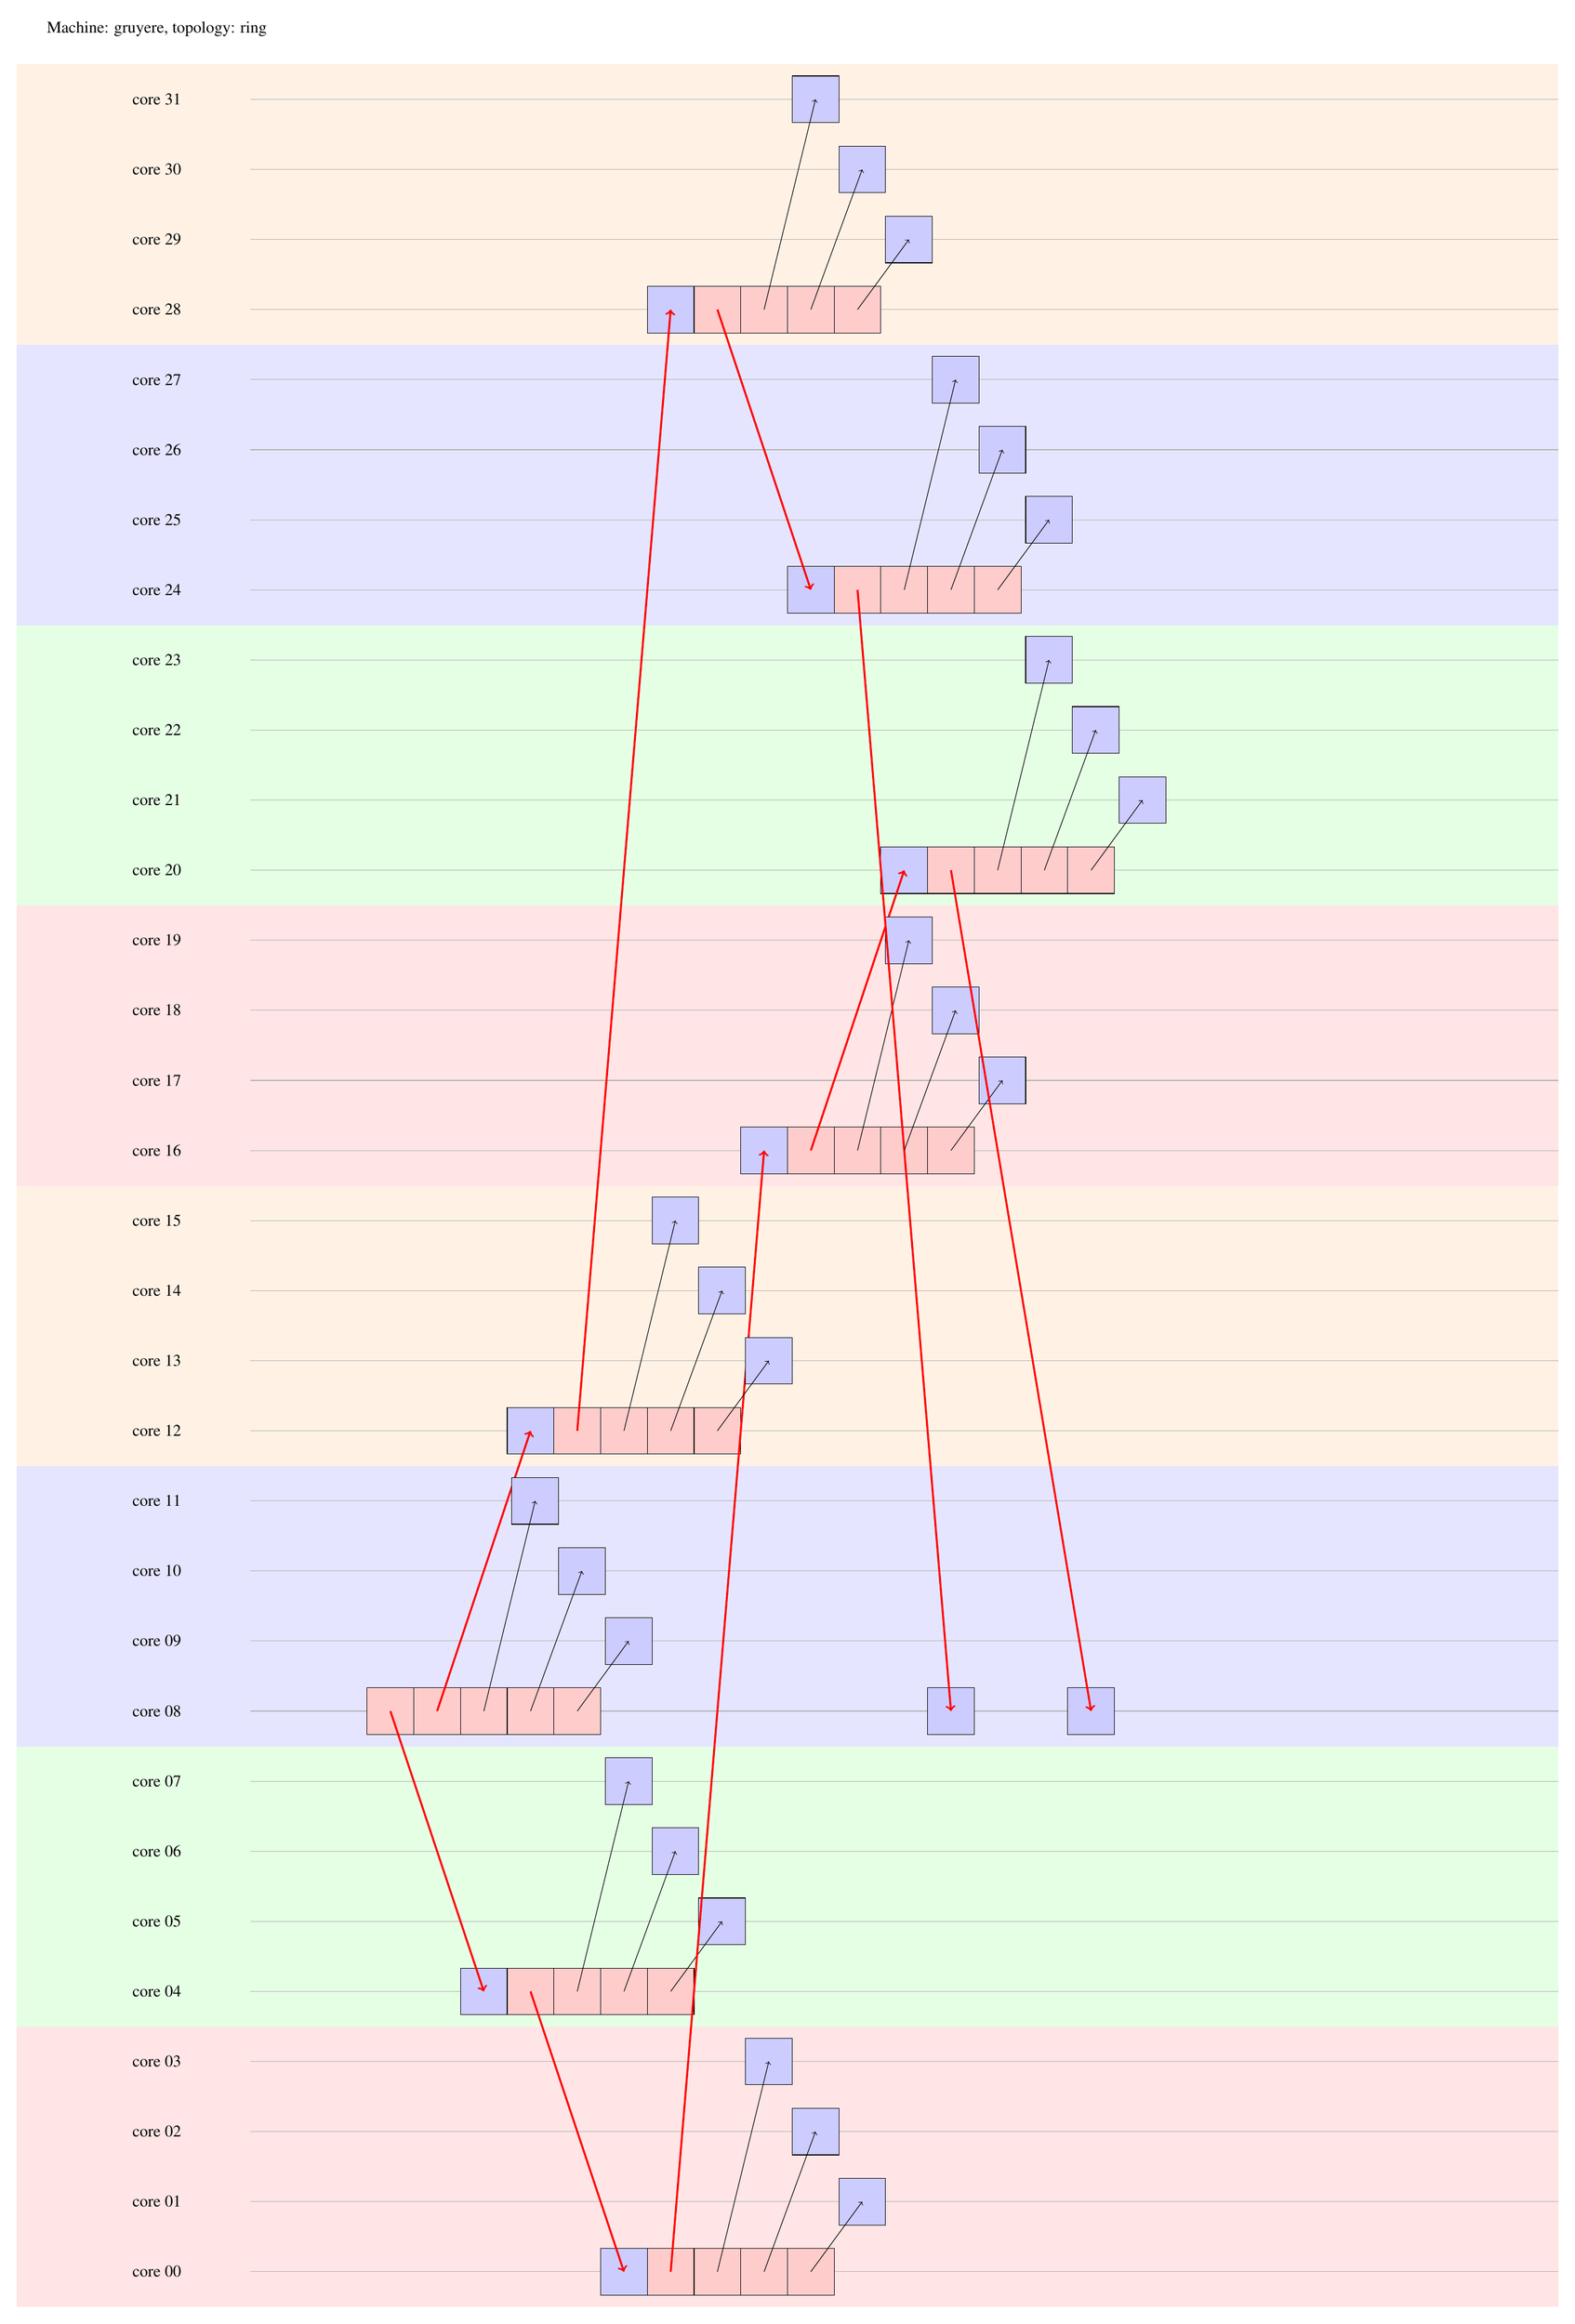
\begin{tikzpicture}[]
  % Insert visualization
  \draw[fill,color=red!10] (-3cm,7.500000mm) rectangle (30cm,-7.500000mm);
\node at (0mm,0mm) {core 00};
\draw[color=black!30] (20mm,0mm) -- (30cm,0mm);
\draw[fill,color=red!10] (-3cm,22.500000mm) rectangle (30cm,7.500000mm);
\node at (0mm,15mm) {core 01};
\draw[color=black!30] (20mm,15mm) -- (30cm,15mm);
\draw[fill,color=red!10] (-3cm,37.500000mm) rectangle (30cm,22.500000mm);
\node at (0mm,30mm) {core 02};
\draw[color=black!30] (20mm,30mm) -- (30cm,30mm);
\draw[fill,color=red!10] (-3cm,52.500000mm) rectangle (30cm,37.500000mm);
\node at (0mm,45mm) {core 03};
\draw[color=black!30] (20mm,45mm) -- (30cm,45mm);
\draw[fill,color=green!10] (-3cm,67.500000mm) rectangle (30cm,52.500000mm);
\node at (0mm,60mm) {core 04};
\draw[color=black!30] (20mm,60mm) -- (30cm,60mm);
\draw[fill,color=green!10] (-3cm,82.500000mm) rectangle (30cm,67.500000mm);
\node at (0mm,75mm) {core 05};
\draw[color=black!30] (20mm,75mm) -- (30cm,75mm);
\draw[fill,color=green!10] (-3cm,97.500000mm) rectangle (30cm,82.500000mm);
\node at (0mm,90mm) {core 06};
\draw[color=black!30] (20mm,90mm) -- (30cm,90mm);
\draw[fill,color=green!10] (-3cm,112.500000mm) rectangle (30cm,97.500000mm);
\node at (0mm,105mm) {core 07};
\draw[color=black!30] (20mm,105mm) -- (30cm,105mm);
\draw[fill,color=blue!10] (-3cm,127.500000mm) rectangle (30cm,112.500000mm);
\node at (0mm,120mm) {core 08};
\draw[color=black!30] (20mm,120mm) -- (30cm,120mm);
\draw[fill,color=blue!10] (-3cm,142.500000mm) rectangle (30cm,127.500000mm);
\node at (0mm,135mm) {core 09};
\draw[color=black!30] (20mm,135mm) -- (30cm,135mm);
\draw[fill,color=blue!10] (-3cm,157.500000mm) rectangle (30cm,142.500000mm);
\node at (0mm,150mm) {core 10};
\draw[color=black!30] (20mm,150mm) -- (30cm,150mm);
\draw[fill,color=blue!10] (-3cm,172.500000mm) rectangle (30cm,157.500000mm);
\node at (0mm,165mm) {core 11};
\draw[color=black!30] (20mm,165mm) -- (30cm,165mm);
\draw[fill,color=orange!10] (-3cm,187.500000mm) rectangle (30cm,172.500000mm);
\node at (0mm,180mm) {core 12};
\draw[color=black!30] (20mm,180mm) -- (30cm,180mm);
\draw[fill,color=orange!10] (-3cm,202.500000mm) rectangle (30cm,187.500000mm);
\node at (0mm,195mm) {core 13};
\draw[color=black!30] (20mm,195mm) -- (30cm,195mm);
\draw[fill,color=orange!10] (-3cm,217.500000mm) rectangle (30cm,202.500000mm);
\node at (0mm,210mm) {core 14};
\draw[color=black!30] (20mm,210mm) -- (30cm,210mm);
\draw[fill,color=orange!10] (-3cm,232.500000mm) rectangle (30cm,217.500000mm);
\node at (0mm,225mm) {core 15};
\draw[color=black!30] (20mm,225mm) -- (30cm,225mm);
\draw[fill,color=red!10] (-3cm,247.500000mm) rectangle (30cm,232.500000mm);
\node at (0mm,240mm) {core 16};
\draw[color=black!30] (20mm,240mm) -- (30cm,240mm);
\draw[fill,color=red!10] (-3cm,262.500000mm) rectangle (30cm,247.500000mm);
\node at (0mm,255mm) {core 17};
\draw[color=black!30] (20mm,255mm) -- (30cm,255mm);
\draw[fill,color=red!10] (-3cm,277.500000mm) rectangle (30cm,262.500000mm);
\node at (0mm,270mm) {core 18};
\draw[color=black!30] (20mm,270mm) -- (30cm,270mm);
\draw[fill,color=red!10] (-3cm,292.500000mm) rectangle (30cm,277.500000mm);
\node at (0mm,285mm) {core 19};
\draw[color=black!30] (20mm,285mm) -- (30cm,285mm);
\draw[fill,color=green!10] (-3cm,307.500000mm) rectangle (30cm,292.500000mm);
\node at (0mm,300mm) {core 20};
\draw[color=black!30] (20mm,300mm) -- (30cm,300mm);
\draw[fill,color=green!10] (-3cm,322.500000mm) rectangle (30cm,307.500000mm);
\node at (0mm,315mm) {core 21};
\draw[color=black!30] (20mm,315mm) -- (30cm,315mm);
\draw[fill,color=green!10] (-3cm,337.500000mm) rectangle (30cm,322.500000mm);
\node at (0mm,330mm) {core 22};
\draw[color=black!30] (20mm,330mm) -- (30cm,330mm);
\draw[fill,color=green!10] (-3cm,352.500000mm) rectangle (30cm,337.500000mm);
\node at (0mm,345mm) {core 23};
\draw[color=black!30] (20mm,345mm) -- (30cm,345mm);
\draw[fill,color=blue!10] (-3cm,367.500000mm) rectangle (30cm,352.500000mm);
\node at (0mm,360mm) {core 24};
\draw[color=black!30] (20mm,360mm) -- (30cm,360mm);
\draw[fill,color=blue!10] (-3cm,382.500000mm) rectangle (30cm,367.500000mm);
\node at (0mm,375mm) {core 25};
\draw[color=black!30] (20mm,375mm) -- (30cm,375mm);
\draw[fill,color=blue!10] (-3cm,397.500000mm) rectangle (30cm,382.500000mm);
\node at (0mm,390mm) {core 26};
\draw[color=black!30] (20mm,390mm) -- (30cm,390mm);
\draw[fill,color=blue!10] (-3cm,412.500000mm) rectangle (30cm,397.500000mm);
\node at (0mm,405mm) {core 27};
\draw[color=black!30] (20mm,405mm) -- (30cm,405mm);
\draw[fill,color=orange!10] (-3cm,427.500000mm) rectangle (30cm,412.500000mm);
\node at (0mm,420mm) {core 28};
\draw[color=black!30] (20mm,420mm) -- (30cm,420mm);
\draw[fill,color=orange!10] (-3cm,442.500000mm) rectangle (30cm,427.500000mm);
\node at (0mm,435mm) {core 29};
\draw[color=black!30] (20mm,435mm) -- (30cm,435mm);
\draw[fill,color=orange!10] (-3cm,457.500000mm) rectangle (30cm,442.500000mm);
\node at (0mm,450mm) {core 30};
\draw[color=black!30] (20mm,450mm) -- (30cm,450mm);
\draw[fill,color=orange!10] (-3cm,472.500000mm) rectangle (30cm,457.500000mm);
\node at (0mm,465mm) {core 31};
\draw[color=black!30] (20mm,465mm) -- (30cm,465mm);
\node at (0mm,480mm) {Machine: gruyere, topology: ring};
\node[draw,fill=red!20,minimum size=10mm] (s_8_4) at (50mm,120mm) {};
\node[draw,fill=red!20,minimum size=10mm] (s_8_12) at (60mm,120mm) {};
\node[draw,fill=red!20,minimum size=10mm] (s_8_11) at (70mm,120mm) {};
\node[draw,fill=red!20,minimum size=10mm] (s_8_10) at (80mm,120mm) {};
\node[draw,fill=red!20,minimum size=10mm] (s_8_9) at (90mm,120mm) {};
\node[draw,fill=blue!20,minimum size=10mm] (r_8_4) at (70mm,60mm) {};
\draw[->,very thick,color=red] (s_8_4.center) -- (r_8_4.center); 
\node[draw,fill=red!20,minimum size=10mm] (s_4_0) at (80mm,60mm) {};
\node[draw,fill=red!20,minimum size=10mm] (s_4_7) at (90mm,60mm) {};
\node[draw,fill=red!20,minimum size=10mm] (s_4_6) at (100mm,60mm) {};
\node[draw,fill=red!20,minimum size=10mm] (s_4_5) at (110mm,60mm) {};
\node[draw,fill=blue!20,minimum size=10mm] (r_8_12) at (80mm,180mm) {};
\draw[->,very thick,color=red] (s_8_12.center) -- (r_8_12.center); 
\node[draw,fill=red!20,minimum size=10mm] (s_12_28) at (90mm,180mm) {};
\node[draw,fill=red!20,minimum size=10mm] (s_12_15) at (100mm,180mm) {};
\node[draw,fill=red!20,minimum size=10mm] (s_12_14) at (110mm,180mm) {};
\node[draw,fill=red!20,minimum size=10mm] (s_12_13) at (120mm,180mm) {};
\node[draw,fill=blue!20,minimum size=10mm] (r_8_11) at (81mm,165mm) {};
\draw[->] (s_8_11.center) -- (r_8_11.center); 
\node[draw,fill=blue!20,minimum size=10mm] (r_8_10) at (91mm,150mm) {};
\draw[->] (s_8_10.center) -- (r_8_10.center); 
\node[draw,fill=blue!20,minimum size=10mm] (r_4_0) at (100mm,0mm) {};
\draw[->,very thick,color=red] (s_4_0.center) -- (r_4_0.center); 
\node[draw,fill=red!20,minimum size=10mm] (s_0_16) at (110mm,0mm) {};
\node[draw,fill=red!20,minimum size=10mm] (s_0_3) at (120mm,0mm) {};
\node[draw,fill=red!20,minimum size=10mm] (s_0_2) at (130mm,0mm) {};
\node[draw,fill=red!20,minimum size=10mm] (s_0_1) at (140mm,0mm) {};
\node[draw,fill=blue!20,minimum size=10mm] (r_4_7) at (101mm,105mm) {};
\draw[->] (s_4_7.center) -- (r_4_7.center); 
\node[draw,fill=blue!20,minimum size=10mm] (r_8_9) at (101mm,135mm) {};
\draw[->] (s_8_9.center) -- (r_8_9.center); 
\node[draw,fill=blue!20,minimum size=10mm] (r_12_28) at (110mm,420mm) {};
\draw[->,very thick,color=red] (s_12_28.center) -- (r_12_28.center); 
\node[draw,fill=red!20,minimum size=10mm] (s_28_24) at (120mm,420mm) {};
\node[draw,fill=red!20,minimum size=10mm] (s_28_31) at (130mm,420mm) {};
\node[draw,fill=red!20,minimum size=10mm] (s_28_30) at (140mm,420mm) {};
\node[draw,fill=red!20,minimum size=10mm] (s_28_29) at (150mm,420mm) {};
\node[draw,fill=blue!20,minimum size=10mm] (r_12_15) at (111mm,225mm) {};
\draw[->] (s_12_15.center) -- (r_12_15.center); 
\node[draw,fill=blue!20,minimum size=10mm] (r_4_6) at (111mm,90mm) {};
\draw[->] (s_4_6.center) -- (r_4_6.center); 
\node[draw,fill=blue!20,minimum size=10mm] (r_4_5) at (121mm,75mm) {};
\draw[->] (s_4_5.center) -- (r_4_5.center); 
\node[draw,fill=blue!20,minimum size=10mm] (r_12_14) at (121mm,210mm) {};
\draw[->] (s_12_14.center) -- (r_12_14.center); 
\node[draw,fill=blue!20,minimum size=10mm] (r_0_16) at (130mm,240mm) {};
\draw[->,very thick,color=red] (s_0_16.center) -- (r_0_16.center); 
\node[draw,fill=red!20,minimum size=10mm] (s_16_20) at (140mm,240mm) {};
\node[draw,fill=red!20,minimum size=10mm] (s_16_19) at (150mm,240mm) {};
\node[draw,fill=red!20,minimum size=10mm] (s_16_18) at (160mm,240mm) {};
\node[draw,fill=red!20,minimum size=10mm] (s_16_17) at (170mm,240mm) {};
\node[draw,fill=blue!20,minimum size=10mm] (r_12_13) at (131mm,195mm) {};
\draw[->] (s_12_13.center) -- (r_12_13.center); 
\node[draw,fill=blue!20,minimum size=10mm] (r_0_3) at (131mm,45mm) {};
\draw[->] (s_0_3.center) -- (r_0_3.center); 
\node[draw,fill=blue!20,minimum size=10mm] (r_28_24) at (140mm,360mm) {};
\draw[->,very thick,color=red] (s_28_24.center) -- (r_28_24.center); 
\node[draw,fill=red!20,minimum size=10mm] (s_24_8) at (150mm,360mm) {};
\node[draw,fill=red!20,minimum size=10mm] (s_24_27) at (160mm,360mm) {};
\node[draw,fill=red!20,minimum size=10mm] (s_24_26) at (170mm,360mm) {};
\node[draw,fill=red!20,minimum size=10mm] (s_24_25) at (180mm,360mm) {};
\node[draw,fill=blue!20,minimum size=10mm] (r_0_2) at (141mm,30mm) {};
\draw[->] (s_0_2.center) -- (r_0_2.center); 
\node[draw,fill=blue!20,minimum size=10mm] (r_28_31) at (141mm,465mm) {};
\draw[->] (s_28_31.center) -- (r_28_31.center); 
\node[draw,fill=blue!20,minimum size=10mm] (r_28_30) at (151mm,450mm) {};
\draw[->] (s_28_30.center) -- (r_28_30.center); 
\node[draw,fill=blue!20,minimum size=10mm] (r_0_1) at (151mm,15mm) {};
\draw[->] (s_0_1.center) -- (r_0_1.center); 
\node[draw,fill=blue!20,minimum size=10mm] (r_16_20) at (160mm,300mm) {};
\draw[->,very thick,color=red] (s_16_20.center) -- (r_16_20.center); 
\node[draw,fill=red!20,minimum size=10mm] (s_20_8) at (170mm,300mm) {};
\node[draw,fill=red!20,minimum size=10mm] (s_20_23) at (180mm,300mm) {};
\node[draw,fill=red!20,minimum size=10mm] (s_20_22) at (190mm,300mm) {};
\node[draw,fill=red!20,minimum size=10mm] (s_20_21) at (200mm,300mm) {};
\node[draw,fill=blue!20,minimum size=10mm] (r_28_29) at (161mm,435mm) {};
\draw[->] (s_28_29.center) -- (r_28_29.center); 
\node[draw,fill=blue!20,minimum size=10mm] (r_16_19) at (161mm,285mm) {};
\draw[->] (s_16_19.center) -- (r_16_19.center); 
\node[draw,fill=blue!20,minimum size=10mm] (r_24_8) at (170mm,120mm) {};
\draw[->,very thick,color=red] (s_24_8.center) -- (r_24_8.center); 
\node[draw,fill=blue!20,minimum size=10mm] (r_24_27) at (171mm,405mm) {};
\draw[->] (s_24_27.center) -- (r_24_27.center); 
\node[draw,fill=blue!20,minimum size=10mm] (r_16_18) at (171mm,270mm) {};
\draw[->] (s_16_18.center) -- (r_16_18.center); 
\node[draw,fill=blue!20,minimum size=10mm] (r_16_17) at (181mm,255mm) {};
\draw[->] (s_16_17.center) -- (r_16_17.center); 
\node[draw,fill=blue!20,minimum size=10mm] (r_24_26) at (181mm,390mm) {};
\draw[->] (s_24_26.center) -- (r_24_26.center); 
\node[draw,fill=blue!20,minimum size=10mm] (r_24_25) at (191mm,375mm) {};
\draw[->] (s_24_25.center) -- (r_24_25.center); 
\node[draw,fill=blue!20,minimum size=10mm] (r_20_23) at (191mm,345mm) {};
\draw[->] (s_20_23.center) -- (r_20_23.center); 
\node[draw,fill=blue!20,minimum size=10mm] (r_20_8) at (200mm,120mm) {};
\draw[->,very thick,color=red] (s_20_8.center) -- (r_20_8.center); 
\node[draw,fill=blue!20,minimum size=10mm] (r_20_22) at (201mm,330mm) {};
\draw[->] (s_20_22.center) -- (r_20_22.center); 
\node[draw,fill=blue!20,minimum size=10mm] (r_20_21) at (211mm,315mm) {};
\draw[->] (s_20_21.center) -- (r_20_21.center); 

\end{tikzpicture}
\newpage
\subsection{sbrinz1}
\newpage
\subsubsection{badtree}
\begin{tikzpicture}[]
  % Insert visualization
  \input{graphs/visu_sbrinz1_badtree}
\end{tikzpicture}
\newpage
\subsubsection{cluster}
\begin{tikzpicture}[]
  % Insert visualization
  \input{graphs/visu_sbrinz1_cluster}
\end{tikzpicture}
\newpage
\subsubsection{mst}
\begin{tikzpicture}[]
  % Insert visualization
  \input{graphs/visu_sbrinz1_mst}
\end{tikzpicture}
\newpage
\subsubsection{bintree}
\begin{tikzpicture}[]
  % Insert visualization
  \input{graphs/visu_sbrinz1_bintree}
\end{tikzpicture}
\newpage
\subsubsection{sequential}
\begin{tikzpicture}[]
  % Insert visualization
  \input{graphs/visu_sbrinz1_sequential}
\end{tikzpicture}
\newpage
\subsubsection{ring}
\begin{tikzpicture}[]
  % Insert visualization
  \input{graphs/visu_sbrinz1_ring}
\end{tikzpicture}


\end{appendices}

\end{document}
